\chapter{Contribution 1: Proposed OCR approaches for Medical Labels}
\clearpage
\label{chap:besoins}
%\setcounter{secnumdepth}{3}

\section{Introduction}
In this chapter, we will present our first contribution, which focuses on developing an automated system for text recognition from medical labels using artificial intelligence techniques. Our approach combines 3 OCR models to accurately extract vital information from medical labels. In the following sections, we will describe the tools and technologies used in our case study, the implementation of our proposed approaches, and the experimental setup. Finally, we will present the results and a comparative analysis of the performance of the three OCR engines used in this study.%corrected


\section{Contributions} 
%\textcolor{red}{This should come in chapter 3 after introduction}
The key contributions of our study are as follows:
\begin{itemize}

\item An expanded dataset size, where we collected more medical label images for the study.

\item A manually annotated dataset of medical label images, encompassing diverse formats, fonts, and imaging conditions to support domain-specific OCR fine-tuning.

\item The fine-tuning and evaluation of three OCR tools: Tesseract v4 (LSTM-based), EasyOCR (CRAFT+CRNN), and Microsoft TrOCR (transformer-based), on the custom dataset.

\item An analysis of preprocessing techniques and annotation strategies that improve recognition robustness for challenging medical label imagery.

\item Hyperparameter Optimization on all the proposed OCR Models using Optuna and Genetic Algorithms (see chapter 4).

\item Comparative study of models' performance demonstrating improvements over default, off-the-shelf OCR and Optimized Models in the context of medical label recognition (see chapter 4).
\end{itemize}%corrected


%\section{Proposed OCR models for Medical Labels}

\section{Dataset Description}
Due to the lack of existence of an Algerian Medical labels dataset, the only dataset that we have is an image dataset that is taken from a local pharmacy store named ”Dis Mebarek” in (khemis Miliana-Ain Defla, Algeria), where we took approximately more than 1000 pictures of 300 medications \cite{meghatria2024}. However, because of the poor performance of the pre-trained OCR tools on this dataset, we have applied fine-tuning to the 3 OCR models used. % and do a comprehensive comparison between the methods to determine which is more accurate and efficient in real-world applications.
In this section, we will describe our dataset that we manually collected, annotated and used for the Model's Fine Tuning. %corrected

\subsection{Dataset Collection}
Given the lack of an Algerian Medical Labels datasets, we expanded the previously mentioned dataset by photographing more madical labels from local pharmacies called
 ”Dis Mebarek” And "Hai Derdara Rue Masjid el Fath" in Khemis Miliana, Ain Defla, Algeria.
This new dataset consists of over 2000 images of different medications. The labels were photographed from various angles and positions, and lighting condition, as illustrated in Figure \ref{fig:labelsposition}.%validated
\vspace{-0.5cm}
\begin{figure}[H]
    \centering
    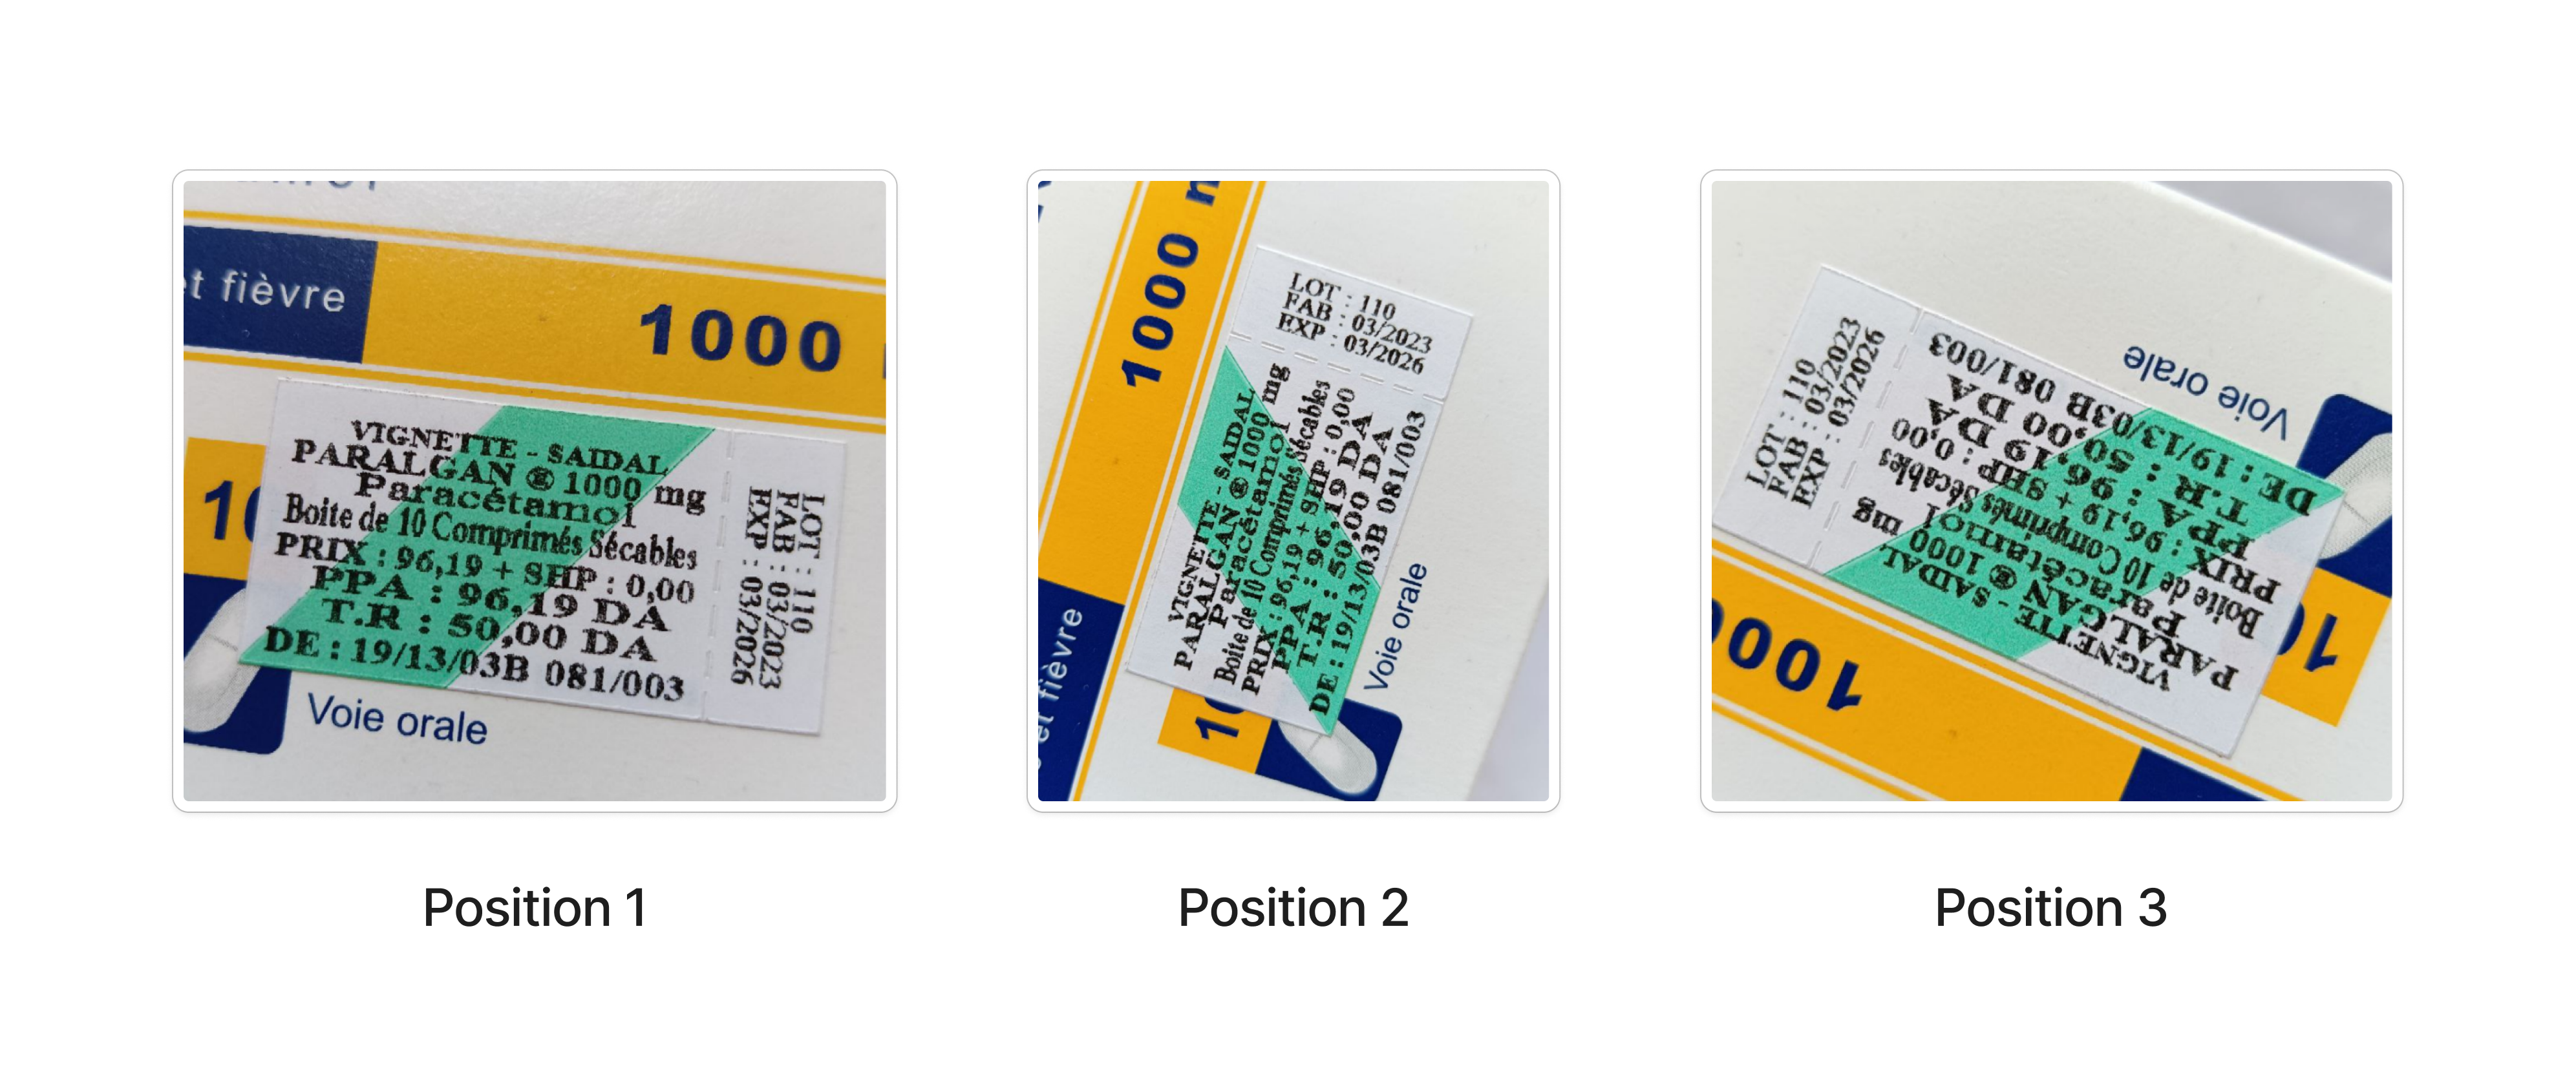
\includegraphics[width=12cm, height=4.5cm]{Figures/Chapter 3/labels_position.png}
    \caption{Different label positions}
    \label{fig:labelsposition}
\end{figure}


The images were taken with the following phone specs:
\begin{itemize} 
    \item \textbf{Redmi Note 10:}
        \begin{itemize}
            \item Dimensions: 160.5 x 74.5 x 8.3 mm
            \item Resolution: 1080 x 2400 pixels
            \item CPU: Octa-core (2x2.2 GHz Kryo 460 Gold \& 6x1.7 GHz Kryo 460 Silver)
            \item Internal Memory: 64GB 6GB RAM
            \item Quad Camera: 48 MP, f/1.8, 26mm (wide), 1/2.0", 0.8µm, PDAF\\
            8 MP, f/2.2, 118˚ (ultrawide), 1/4.0", 1.12µm\\
            2 MP, f/2.4, (macro)\\
            2 MP, f/2.4, (depth)
        \end{itemize}
        
    \item \textbf{Samsung Galaxy S21 Ultra 5G:}
        \begin{itemize}
            \item Dimensions: 165.1 x 75.6 x 8.9 mm
            \item Resolution: 1440 x 3200 pixels
            \item CPU: Octa-core (1x2.9 GHz Cortex-X1 \& 3x2.8 GHz Cortex-A78 \& 4x2.2 GHz Cortex-A55)
            \item Internal Memory: 128GB 12GB RAM
            \item Quad Camera: 108 MP, f/1.8, 26mm (wide), 1/1.33", 0.8µm, PDAF, Laser AF, OIS\\
            10 MP, f/4.9, 240mm (periscope telephoto), 1/3.24", 1.22µm, Dual Pixel PDAF, OIS, 10x optical zoom\\
            10 MP, f/2.4, 70mm (telephoto), 1/3.24", 1.22µm, Dual Pixel PDAF, OIS, 3x optical zoom\\
            12 MP, f/2.2, 13mm, 120˚ (ultrawide), 1/2.55", 1.4µm, Super Steady video
        \end{itemize}

    \item \textbf{Realme 8i:}
        \begin{itemize}
            \item Dimensions: 164.1 x 75.5 x 8.5 mm
            \item Resolution: 1080 x 2412 pixels
            \item CPU: Octa-core (2x2.05 GHz Cortex-A76 \& 6x2.0 GHz Cortex-A55)
            \item Internal Memory: 64GB 4GB RAM
            \item Triple Camera: 50 MP, f/1.8, 26mm (wide), 1/2.76", 0.64µm, PDAF\\
            2 MP, f/2.4, (macro)\\
            2 MP, f/2.4, (depth)
        \end{itemize}
\end{itemize}


%\end{comment}

\subsection{Dataset Preparation}
Following the data collection, the labels were organized into a tabular format and saved in an Excel File to facilitate later exploration, as shown in the figure \ref{fig:dataprep}. This table includes the content of these medical labels written from left to right, where each vertical and horizontal part is written separately.
Each cell contains the lines of text that are written in that part of the medical label (Excluding Logos), and each line of text is separated by a semicolon (;) to distinguish the lines from each other.

\begin{figure}[H]
    \centering
    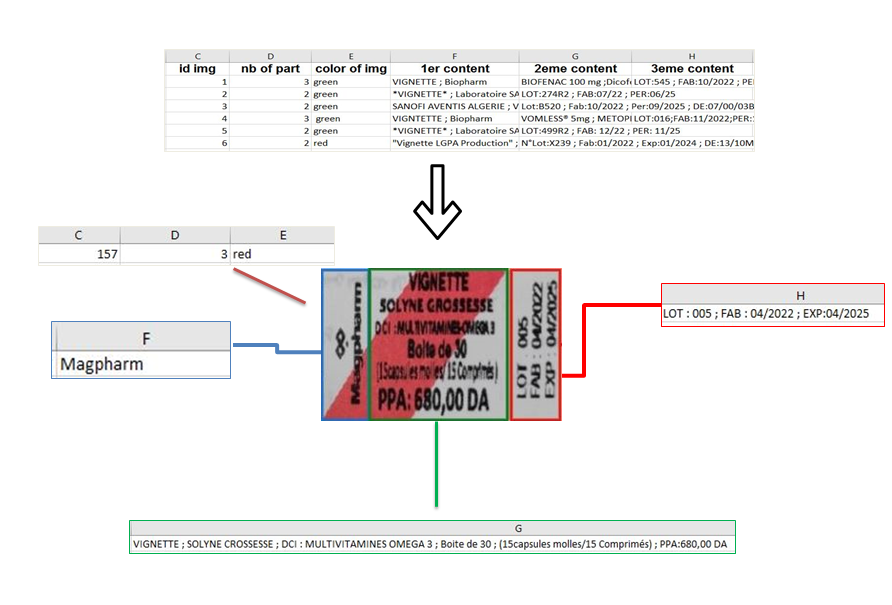
\includegraphics[width=0.75\textwidth]{Figures/Chapter 3/Medical labels documentation.png}
    \caption{Dataset preparation: Tabular documentation}
    \label{fig:dataprep}
\end{figure}

\subsubsection{Dataset Annotation}
\subsubsection*{\textit{Ground Truth}}
In order to fine-tune the OCR models, we would first need to create the ground truth that will serve as our training data. 
After documenting the content of the labels, we used a script that takes the Excel file containing the content of the medical labels and it creates Text files (.Txt) containing the lines of text that are written in the file, and using the semicolon it can seperate each line individually, creating our ground truth labels, as shown in figure \ref{fig:excelintofiles}.

\begin{figure}[H]
    \centering
    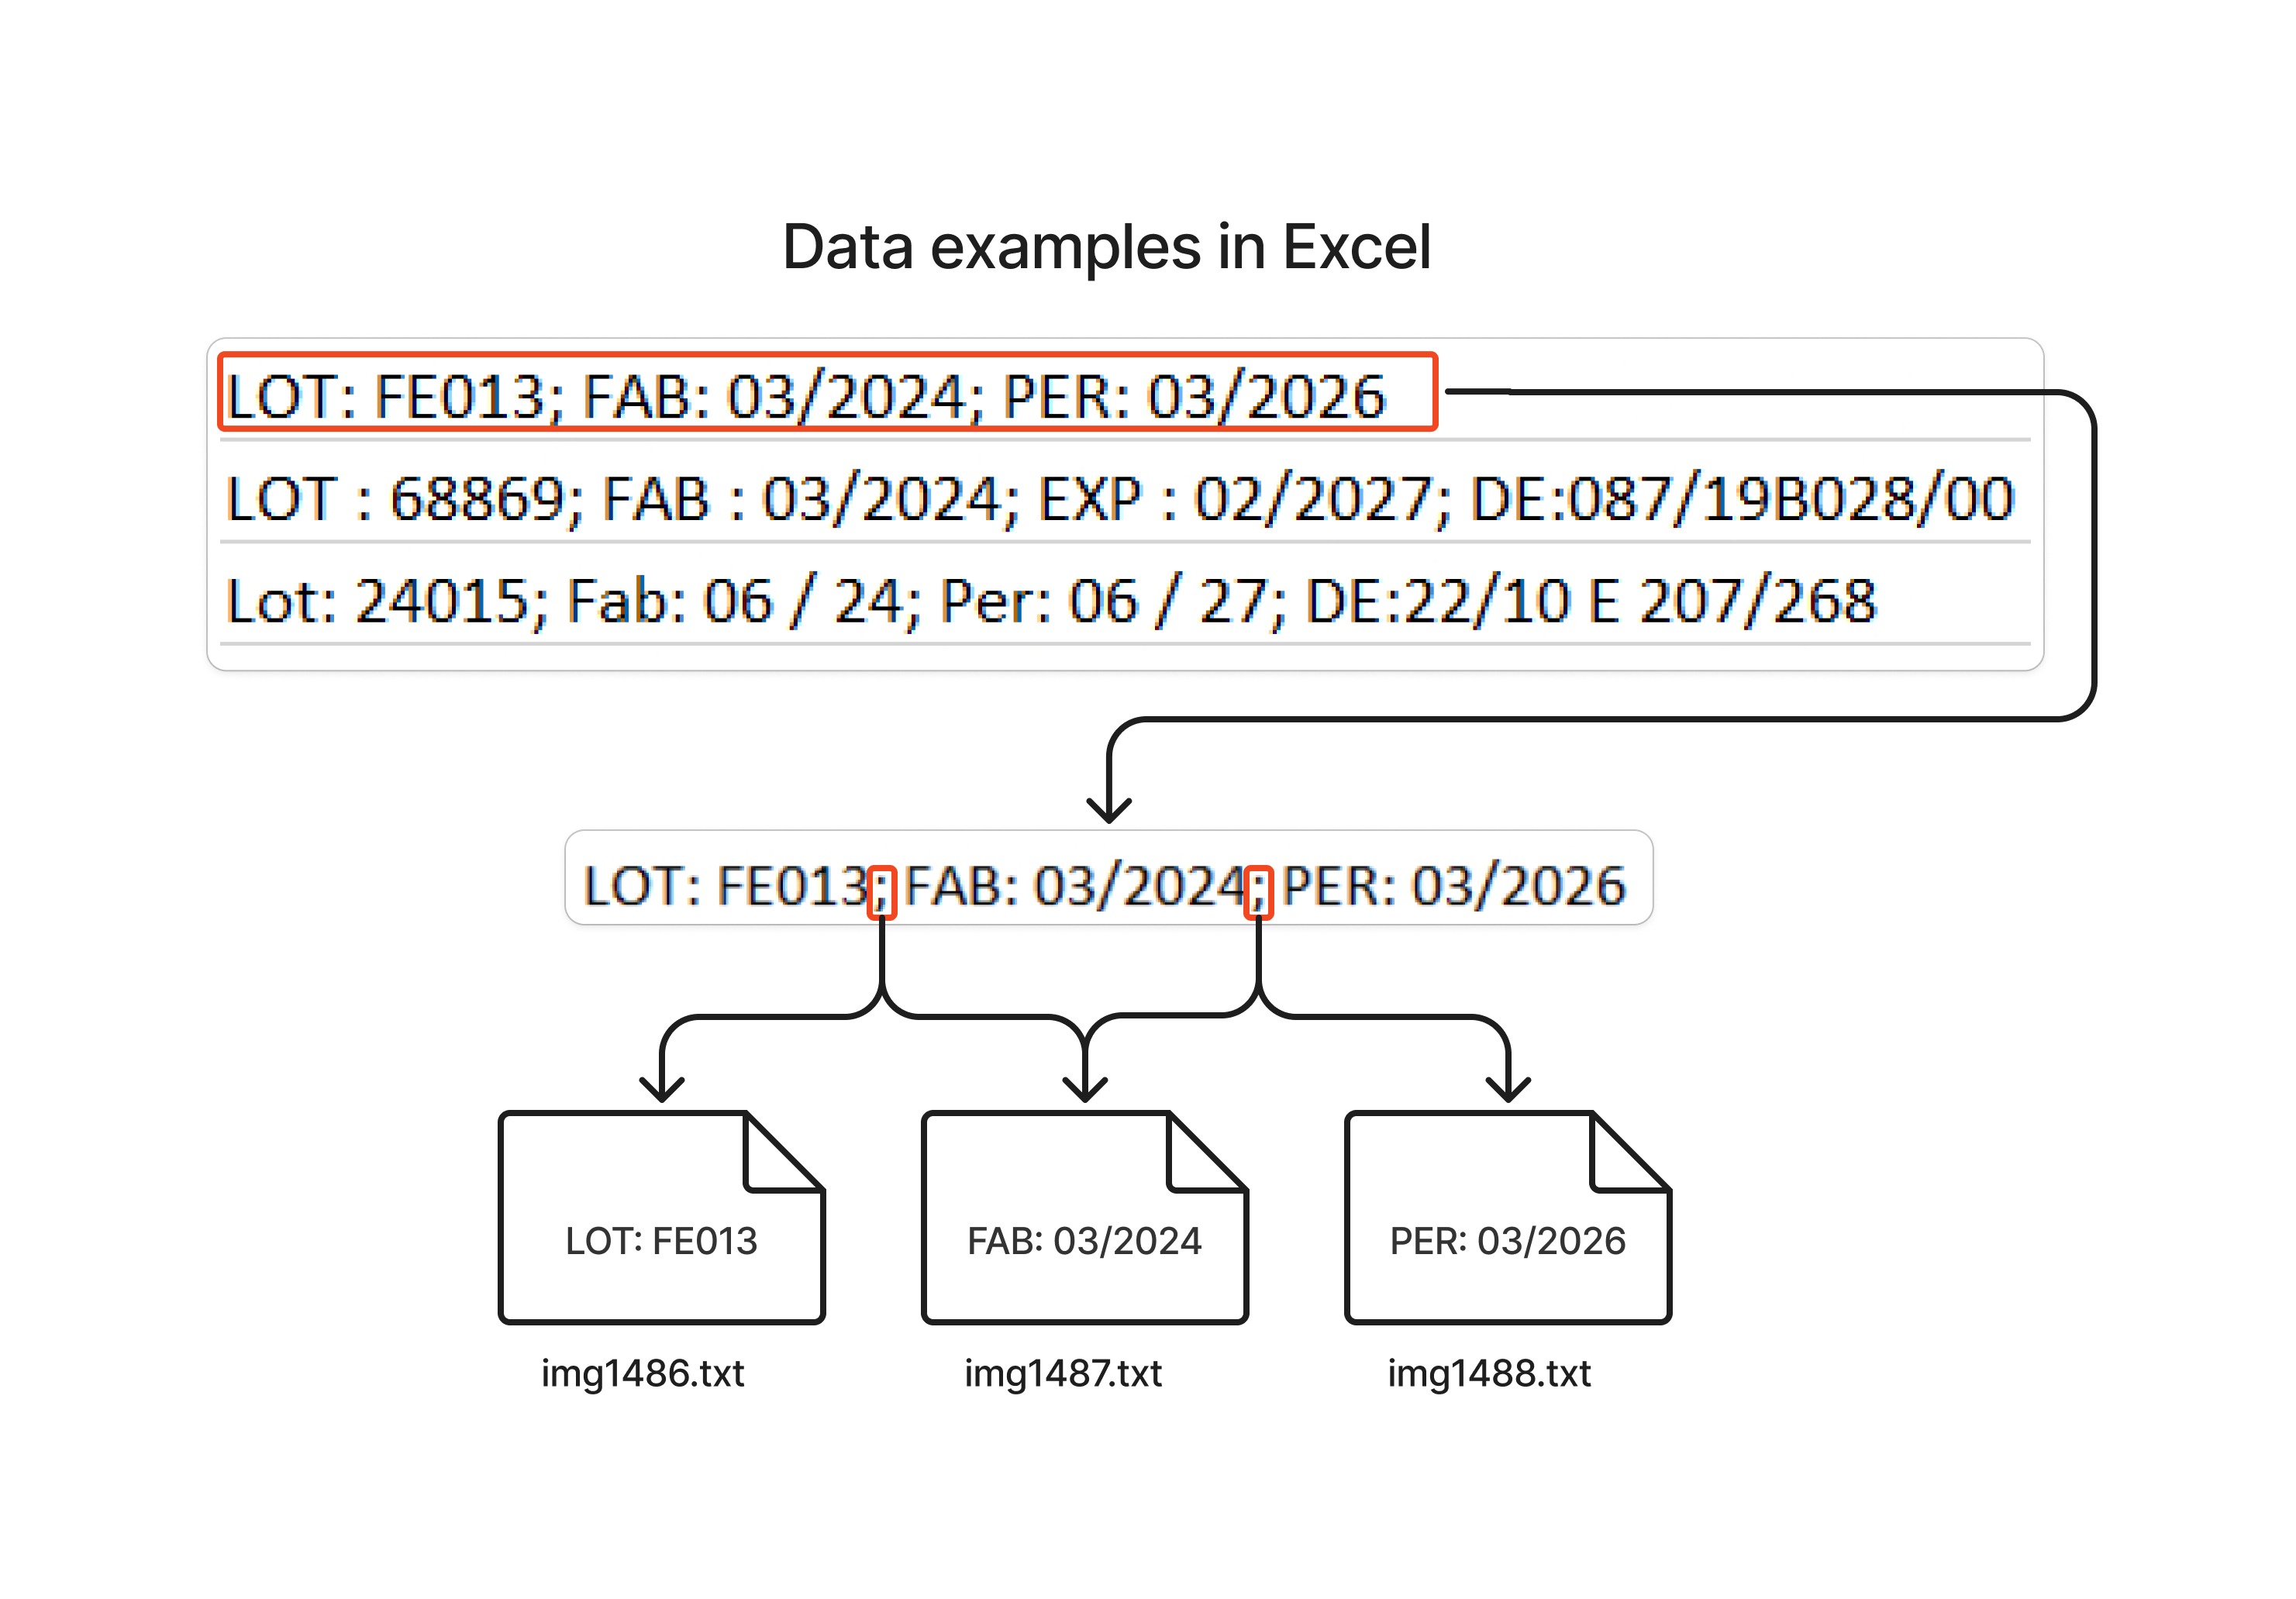
\includegraphics[width=0.95\textwidth]{Figures/Chapter 3/excel_into_files.png}
    \caption{The process of turning Excel into .Txt Files}
    \label{fig:excelintofiles}
\end{figure}
\vspace{-0.5cm}

\subsubsection*{\textit{Input Images (Features)}}
The next step in the Dataset annotation would be to create images of the segmented lines of text, which will serve as our input features for the models.
This is done by segmenting all the lines of text in the photographed medical label images using a Snipping Tool then they are saved in the dataset. The order of segmenting should be the same order as it is documented in the Excel file to facilitate the process. And it is very important to make sure that the segmented image has the exact same name as the corresponding ground truth file (Text file) because a false ground truth of an image could affect the model's performance and lead to overfitting.

\begin{figure}[H]
    \centering
    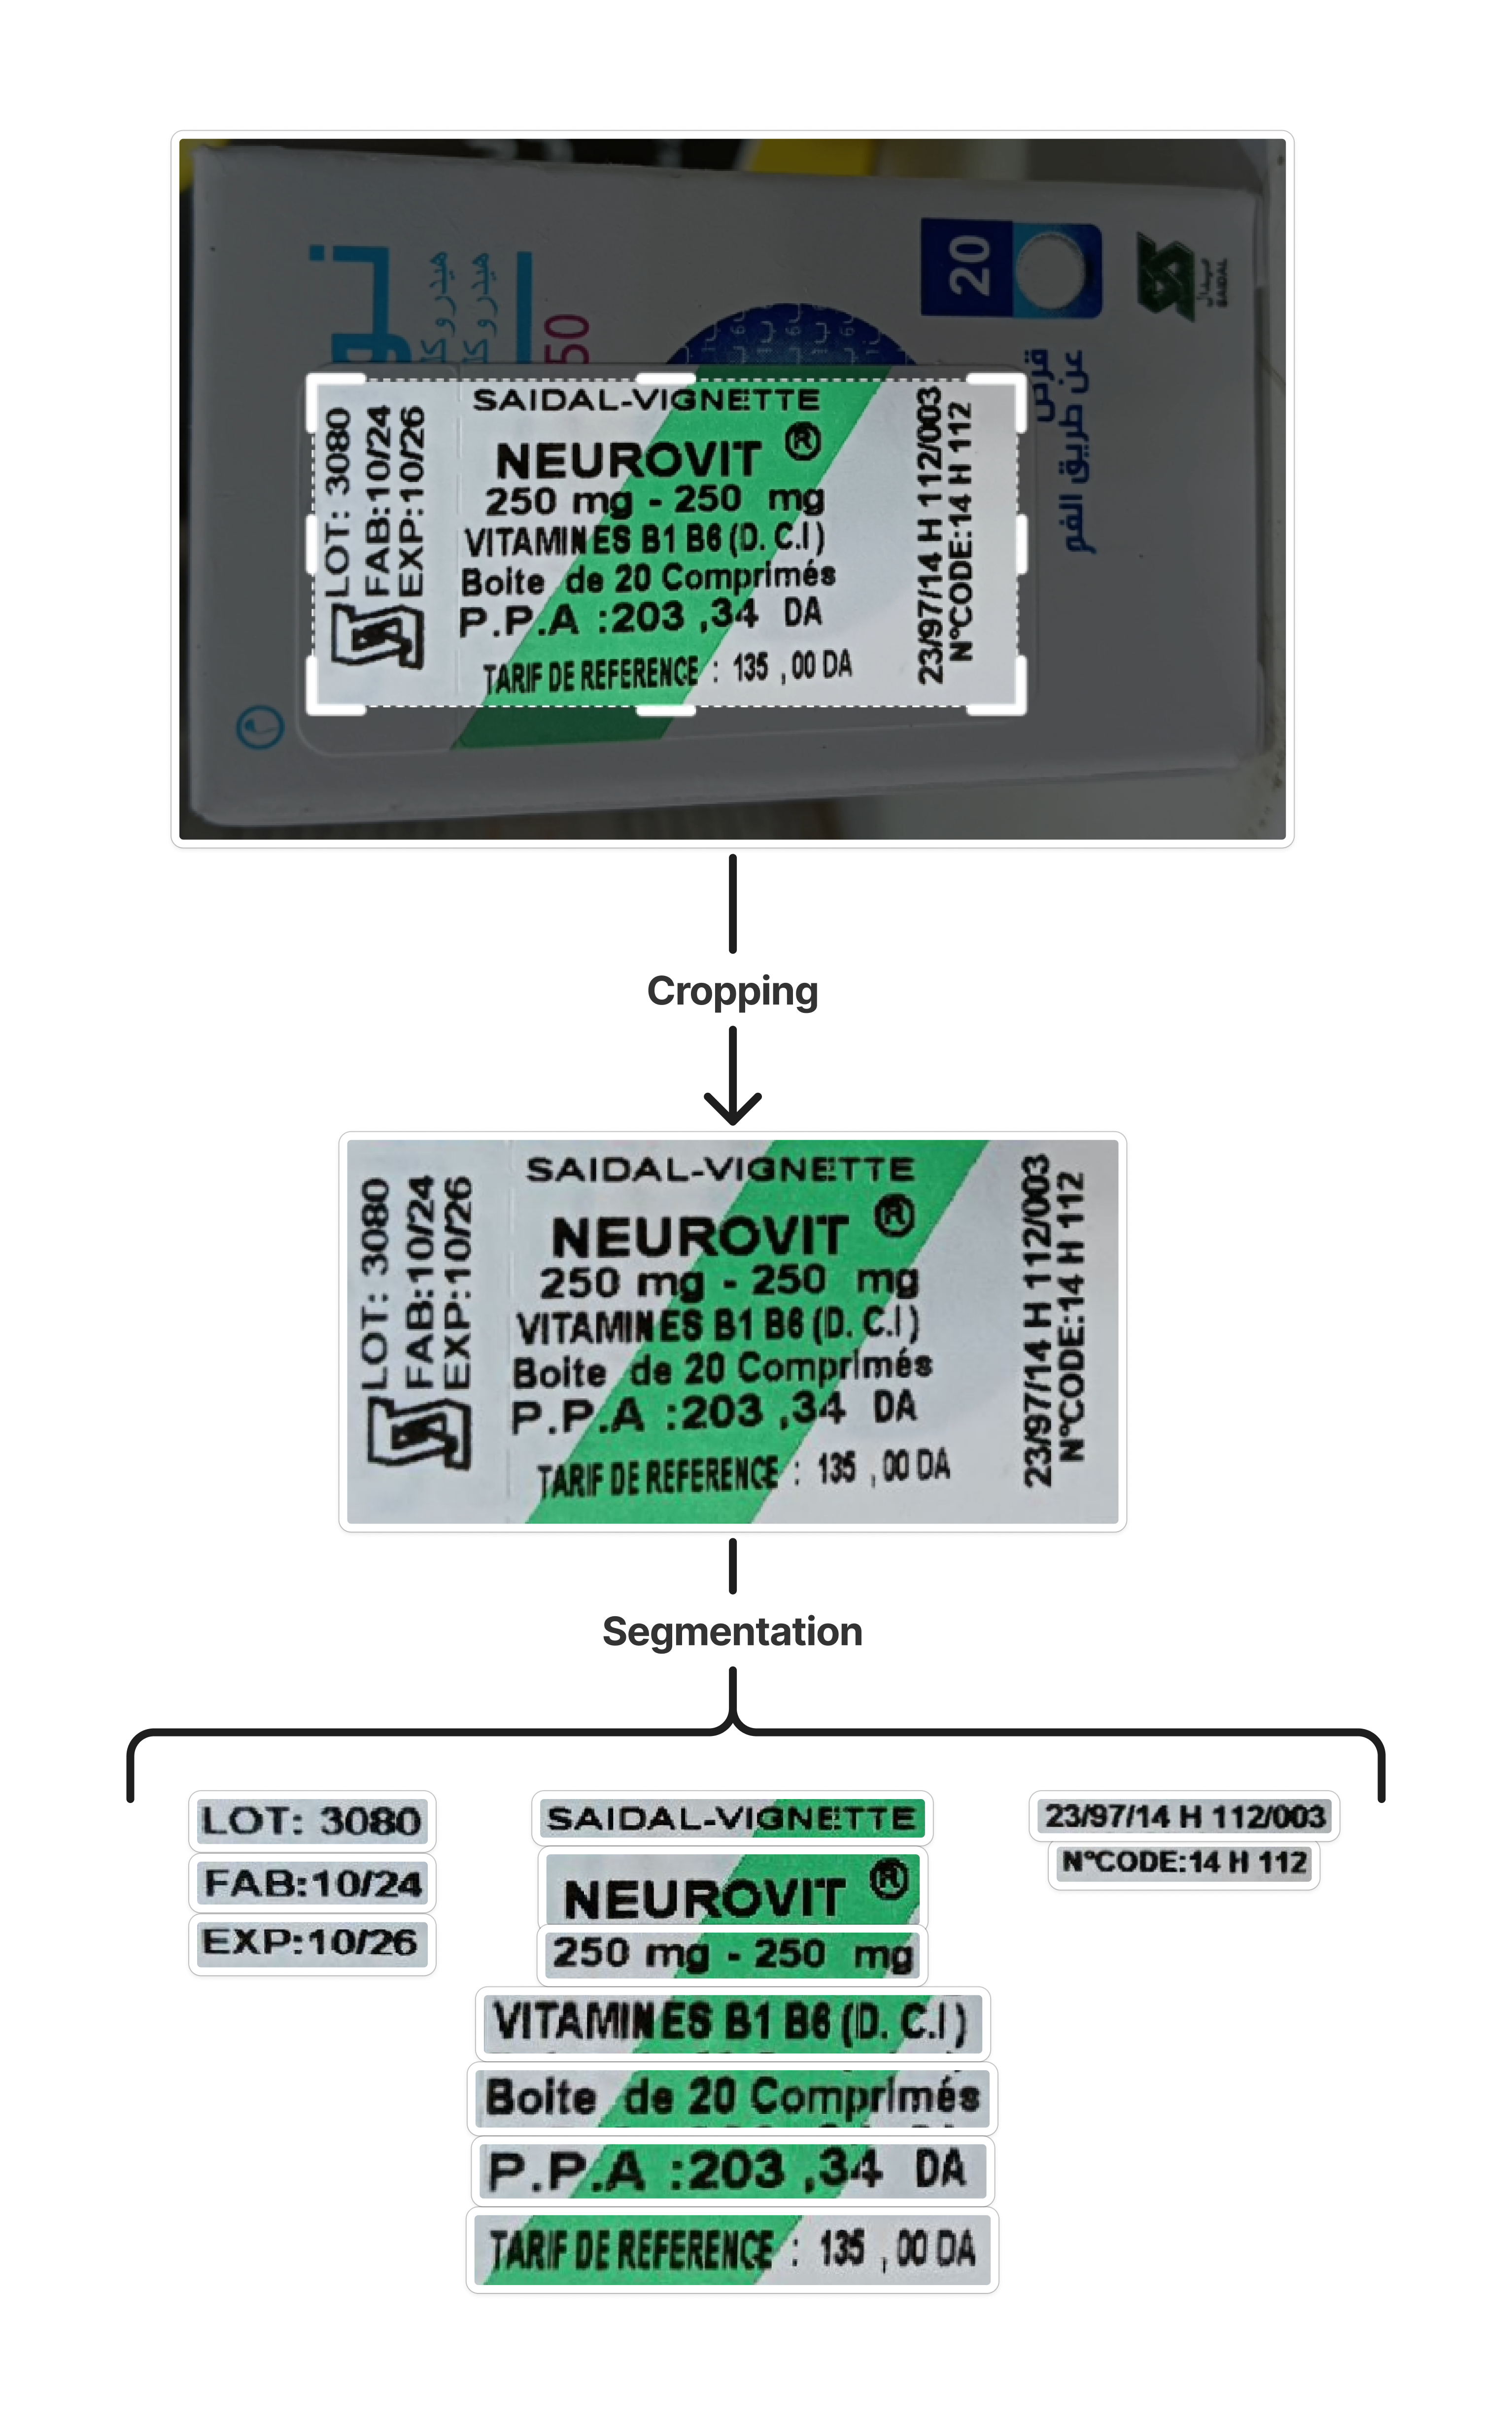
\includegraphics[width=0.5\textwidth]{Figures/Chapter 3/segmented_lines.png}
    \caption{Segmentation of medical labels into lines of text}
    \label{fig:segmentationoflabels}
\end{figure}


\section{Proposed OCR models for Medical Labels}
 %here
 In this section, we will introduce the 3 OCR models that were used and describe their architecture, the Dataset format they require, the Fine-Tuning process and finally a comparison study between our Fine-tuned version and the Standard version.
\subsection{Model 1 - TesseractOCR -: Description and experimental results}

%description, flowchart 
%\subsubsection*{Tesseract Architecture Overview}
In this section, we describe how the Tesseract model is adapted to recognize text from medical labels. Figure \ref{fig:TesseractArchitecture} represents an overview of the architecture of Tesseract OCR and how it is adapted to be applied to the medical labels.

\begin{figure}[tb!]
    \centering
    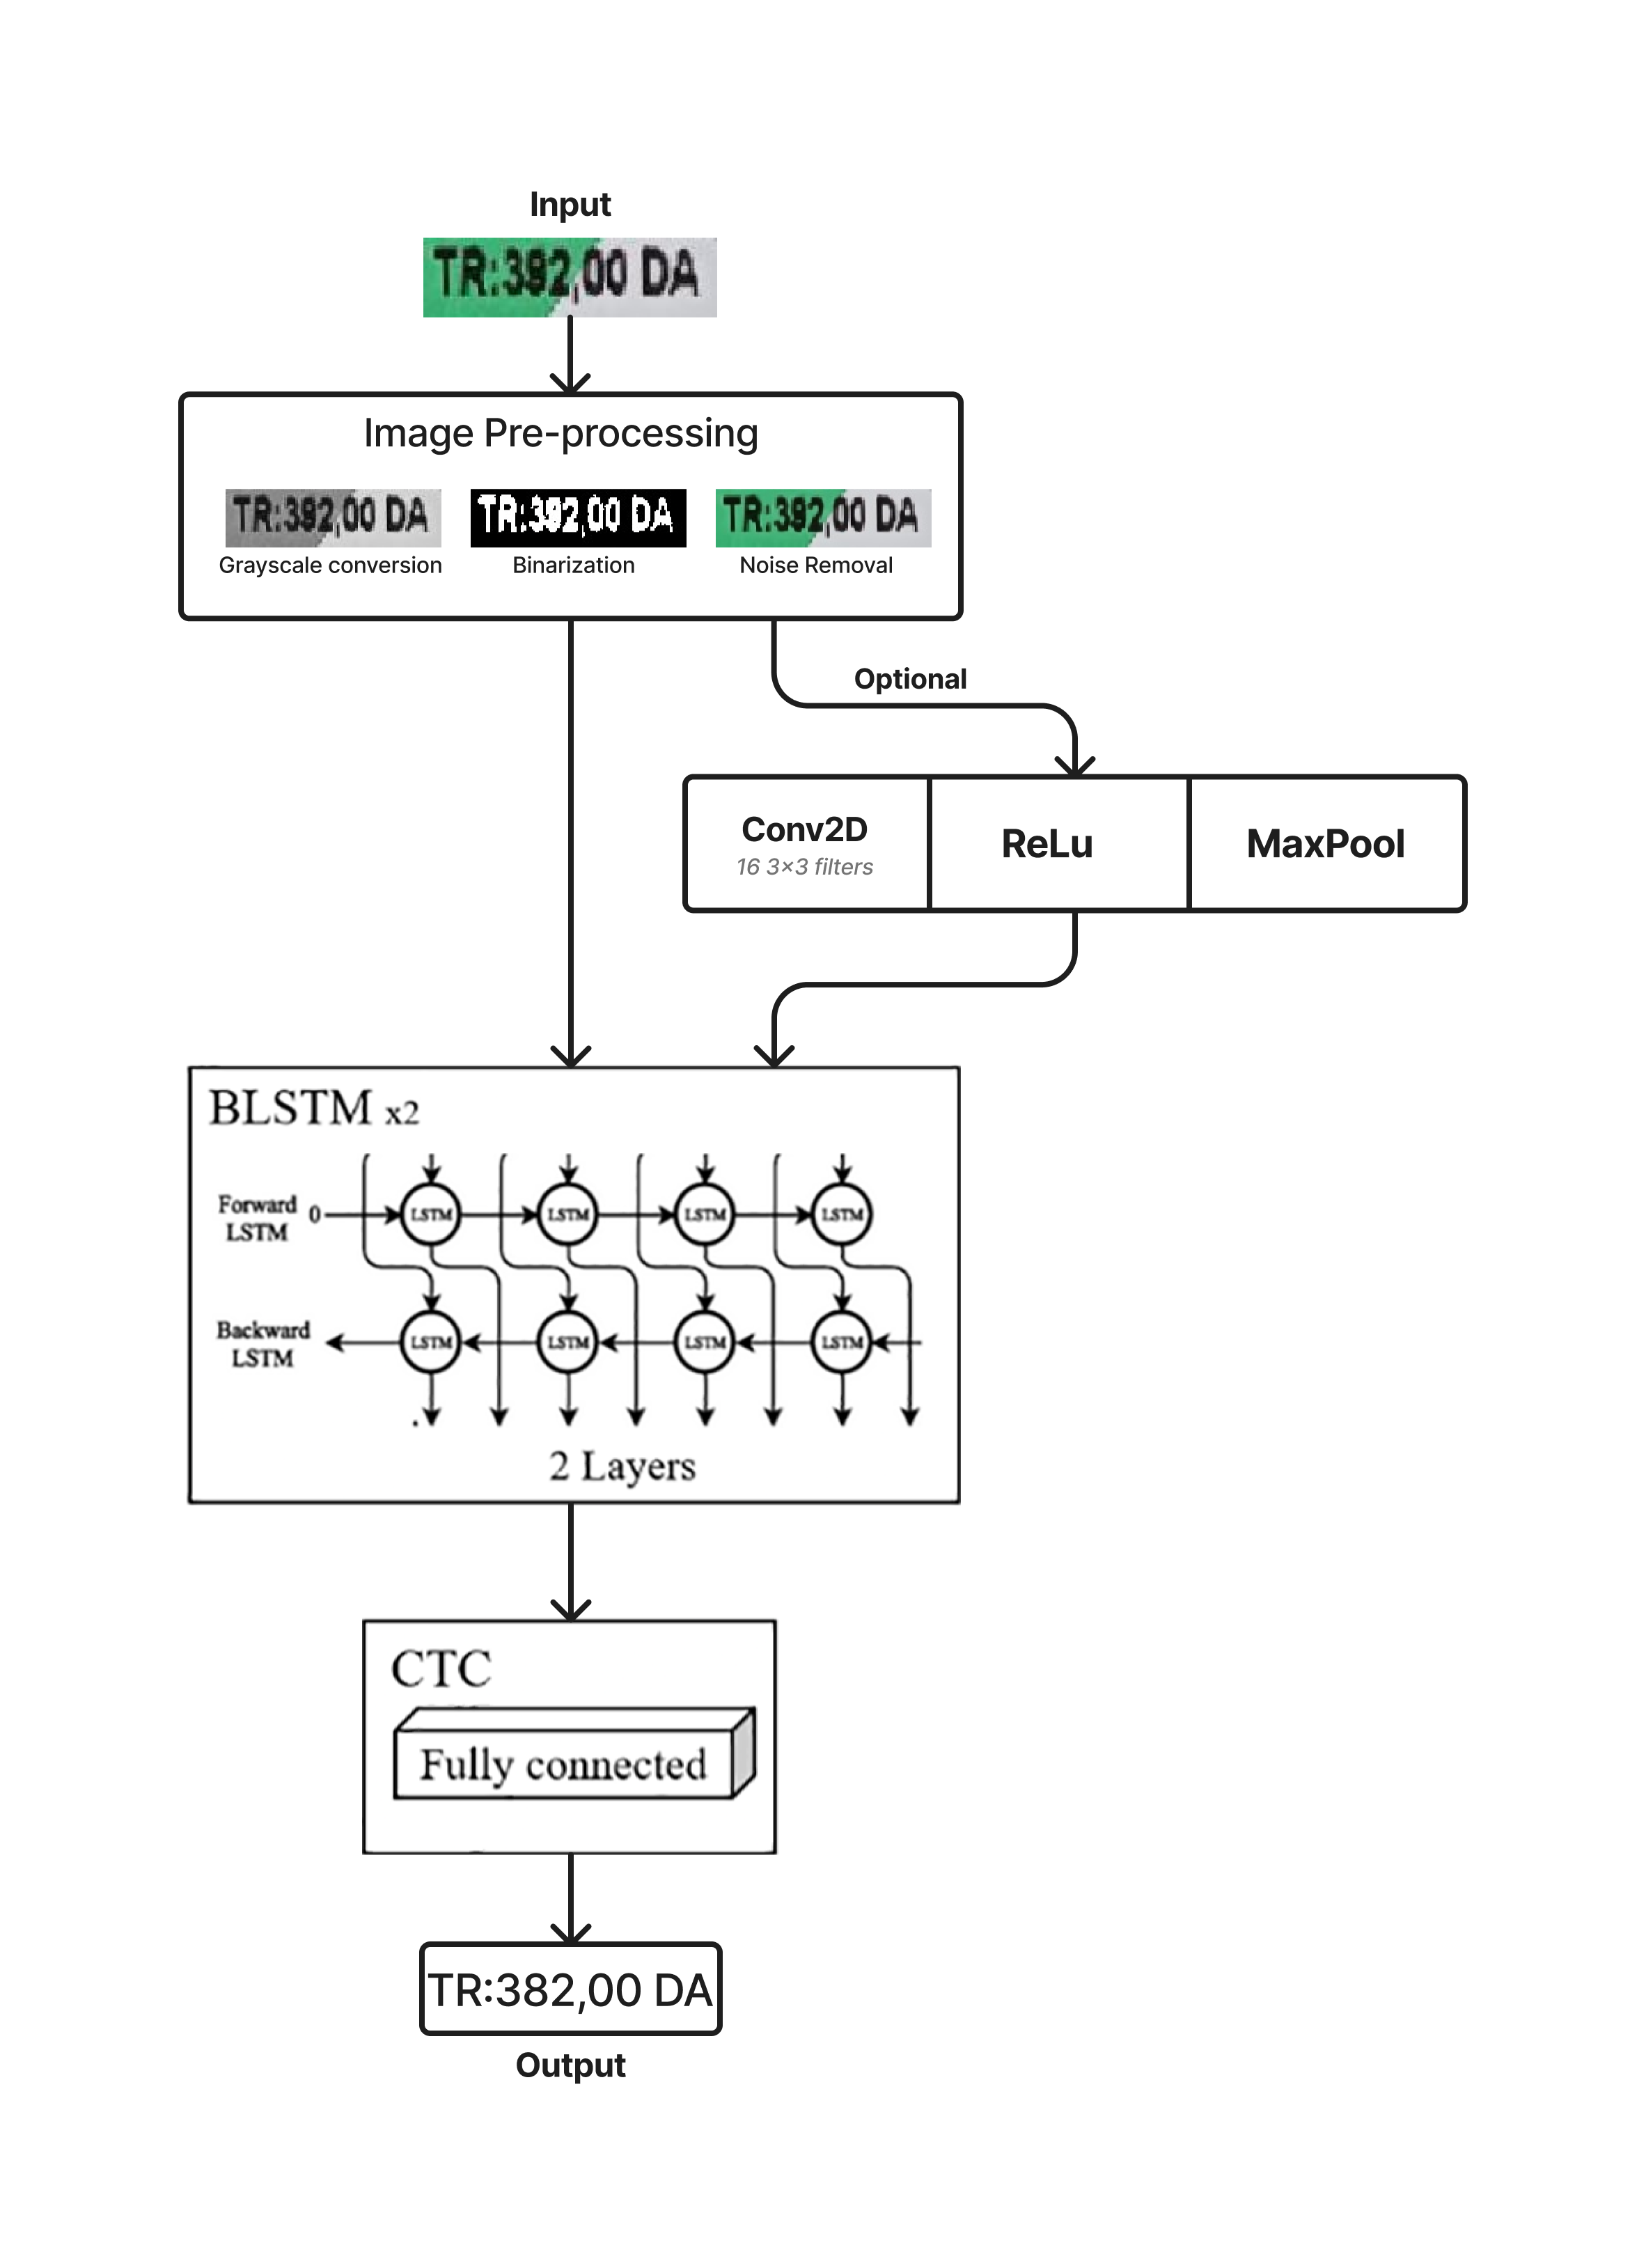
\includegraphics[width=0.75\textwidth]{Figures/Chapter 3/Tesseract_Architecture.png}
    \caption{Tesseract Architecture}
    \label{fig:TesseractArchitecture}
\end{figure}


\subsubsection*{Input}
The input is a cropped image region that contains a line of text, such as a price or medicine label. Tesseract expects the input in grayscale or RGB format and internally resizes or adjusts it for recognition. In this work, images are pre-cropped to focus on the target text.

\subsubsection*{Image Pre-processing}
Before recognition, the input undergoes several preprocessing steps:
\begin{itemize}
    \item \textbf{Grayscale Conversion}: Converts the image to a single-channel grayscale image to simplify computation.
    \item \textbf{Binarization}: Enhances contrast between text and background by converting the image to black and white, using adaptive thresholding or Otsu's method.
    \item \textbf{Noise Removal}: Removes small artifacts and background noise using morphological operations or Gaussian blurring to improve text clarity.
\end{itemize}
These steps help to standardize the input for the recognition pipeline.

\subsubsection*{Optional Convolutional Feature Extraction}
This layer is optionally applied before the recurrent network to extract spatial features from the image:
\begin{itemize}
    \item \textbf{Conv2D Layer}: Applies 16 convolution filters of size $3 \times 3$ to capture local spatial patterns such as edges and curves in characters.
    \item \textbf{ReLU Activation}: Introduces non-linearity to improve learning of complex features.
    \item \textbf{MaxPooling}: Downsamples feature maps by taking the maximum value in local regions, reducing spatial dimensions and retaining important features.
\end{itemize}
This block is lightweight and optional. In many pretrained Tesseract models, it may be disabled or replaced with raw pixel columns.

\subsubsection*{Bidirectional LSTM (BLSTM) Layers}
The core of Tesseract’s OCR engine consists of two stacked Bidirectional Long Short-Term Memory (BLSTM) layers:
\begin{itemize}
    \item Each LSTM processes the image as a sequence of vertical pixel columns (one timestep per column).
    \item The \textbf{forward LSTM} captures dependencies from left to right, while the \textbf{backward LSTM} captures right to left.
    \item The output of both directions is concatenated at each timestep.
\end{itemize}
These layers are responsible for understanding character sequences and their contextual dependencies in the image.

\subsubsection*{Fully Connected + CTC Layer}
After the LSTM layers, the output is passed to a fully connected (dense) layer, which projects the LSTM output at each timestep into a character class space:
\begin{itemize}
    \item The softmax layer assigns probabilities to each possible character (including a blank symbol).
    \item The \textbf{Connectionist Temporal Classification (CTC)} decoder interprets these probabilities to produce the most likely character sequence, without needing aligned labels.
\end{itemize}
CTC allows Tesseract to recognize text lines of variable length with no explicit segmentation.

\subsubsection*{Output}
The final output is the recognized character sequence, reconstructed from the CTC-decoded predictions. In the illustrated example, the network correctly predicts “\texttt{TR:382,00 DA}”.

\subsubsection{Dataset Configuration}

In addition to the Lines of text from Figure \ref{fig:segmentationoflabels}, Tesseract requires Box Files that contain the Ground Truth and their coordinates in the Image.

\begin{figure}[H]
\centering
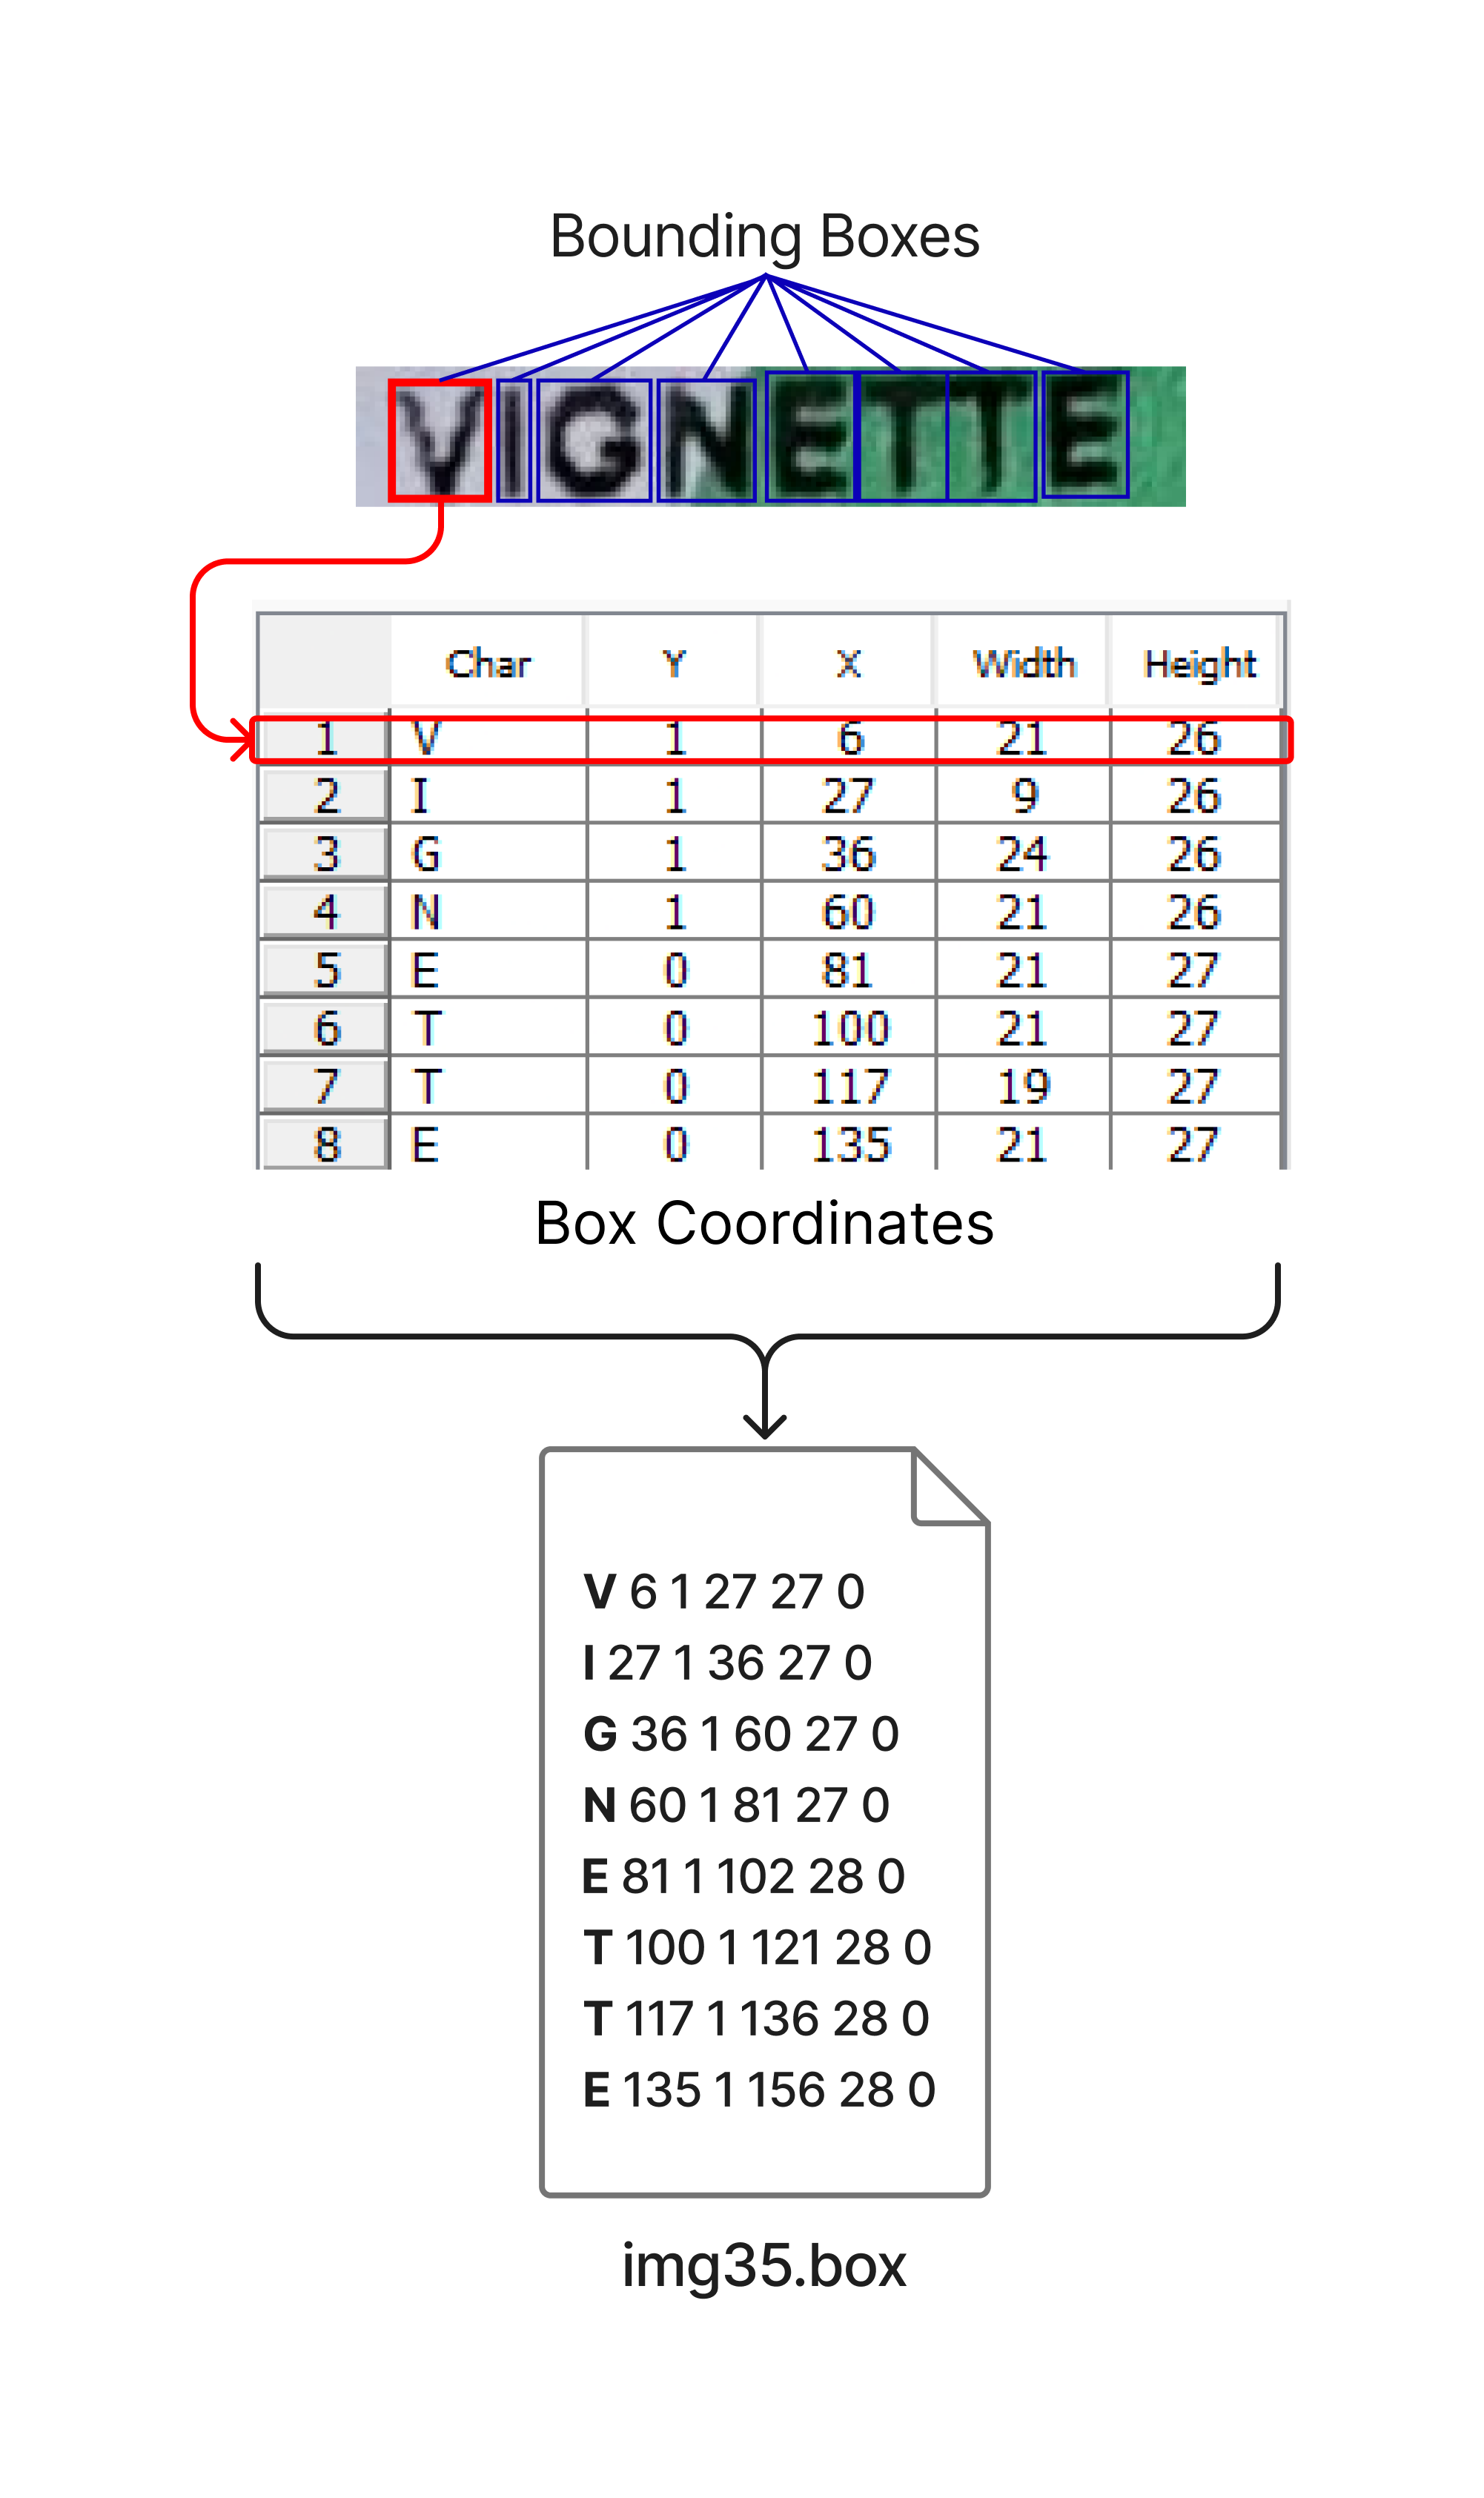
\includegraphics[width=0.50\textwidth]{Figures/Chapter 3/tesseract_Box_Files.png}
\caption{Tesseract Box Files}
\label{fig:tesseractboxfiles}
\end{figure}

The Box Files, as illustrated in Figure \ref{fig:tesseractboxfiles}, provide a mapping between each character in the image and its corresponding bounding box. Each entry in the table represents a single character, along with its top-left coordinates (X, Y), width, and height. These values are derived either manually or through a preprocessing tool, and are essential for supervised OCR training with Tesseract.

Once the bounding box information is prepared, it is converted into the .box file format required by Tesseract. Each line in a .box file includes the character label, the coordinates of the bottom-left and top-right corners of its bounding box, followed by the page number (usually 0 for single-page images). For example, the character V has coordinates (6, 1) for the top-left corner, with a width of 21 and height of 26. These values are transformed into the line:
\begin{center}
\texttt{V 6 1 27 27 0}
\end{center}
This indicates the character "V" spans from (6,1) to (27,27) on the image.

The .box file, typically named to match the image filename (e.g., \texttt{img35.box}), serves as the ground truth reference during the OCR training process. It enables Tesseract to learn the relationship between pixel-level features and character labels.
%\begin{comment}
\begin{figure}[H]
\centering
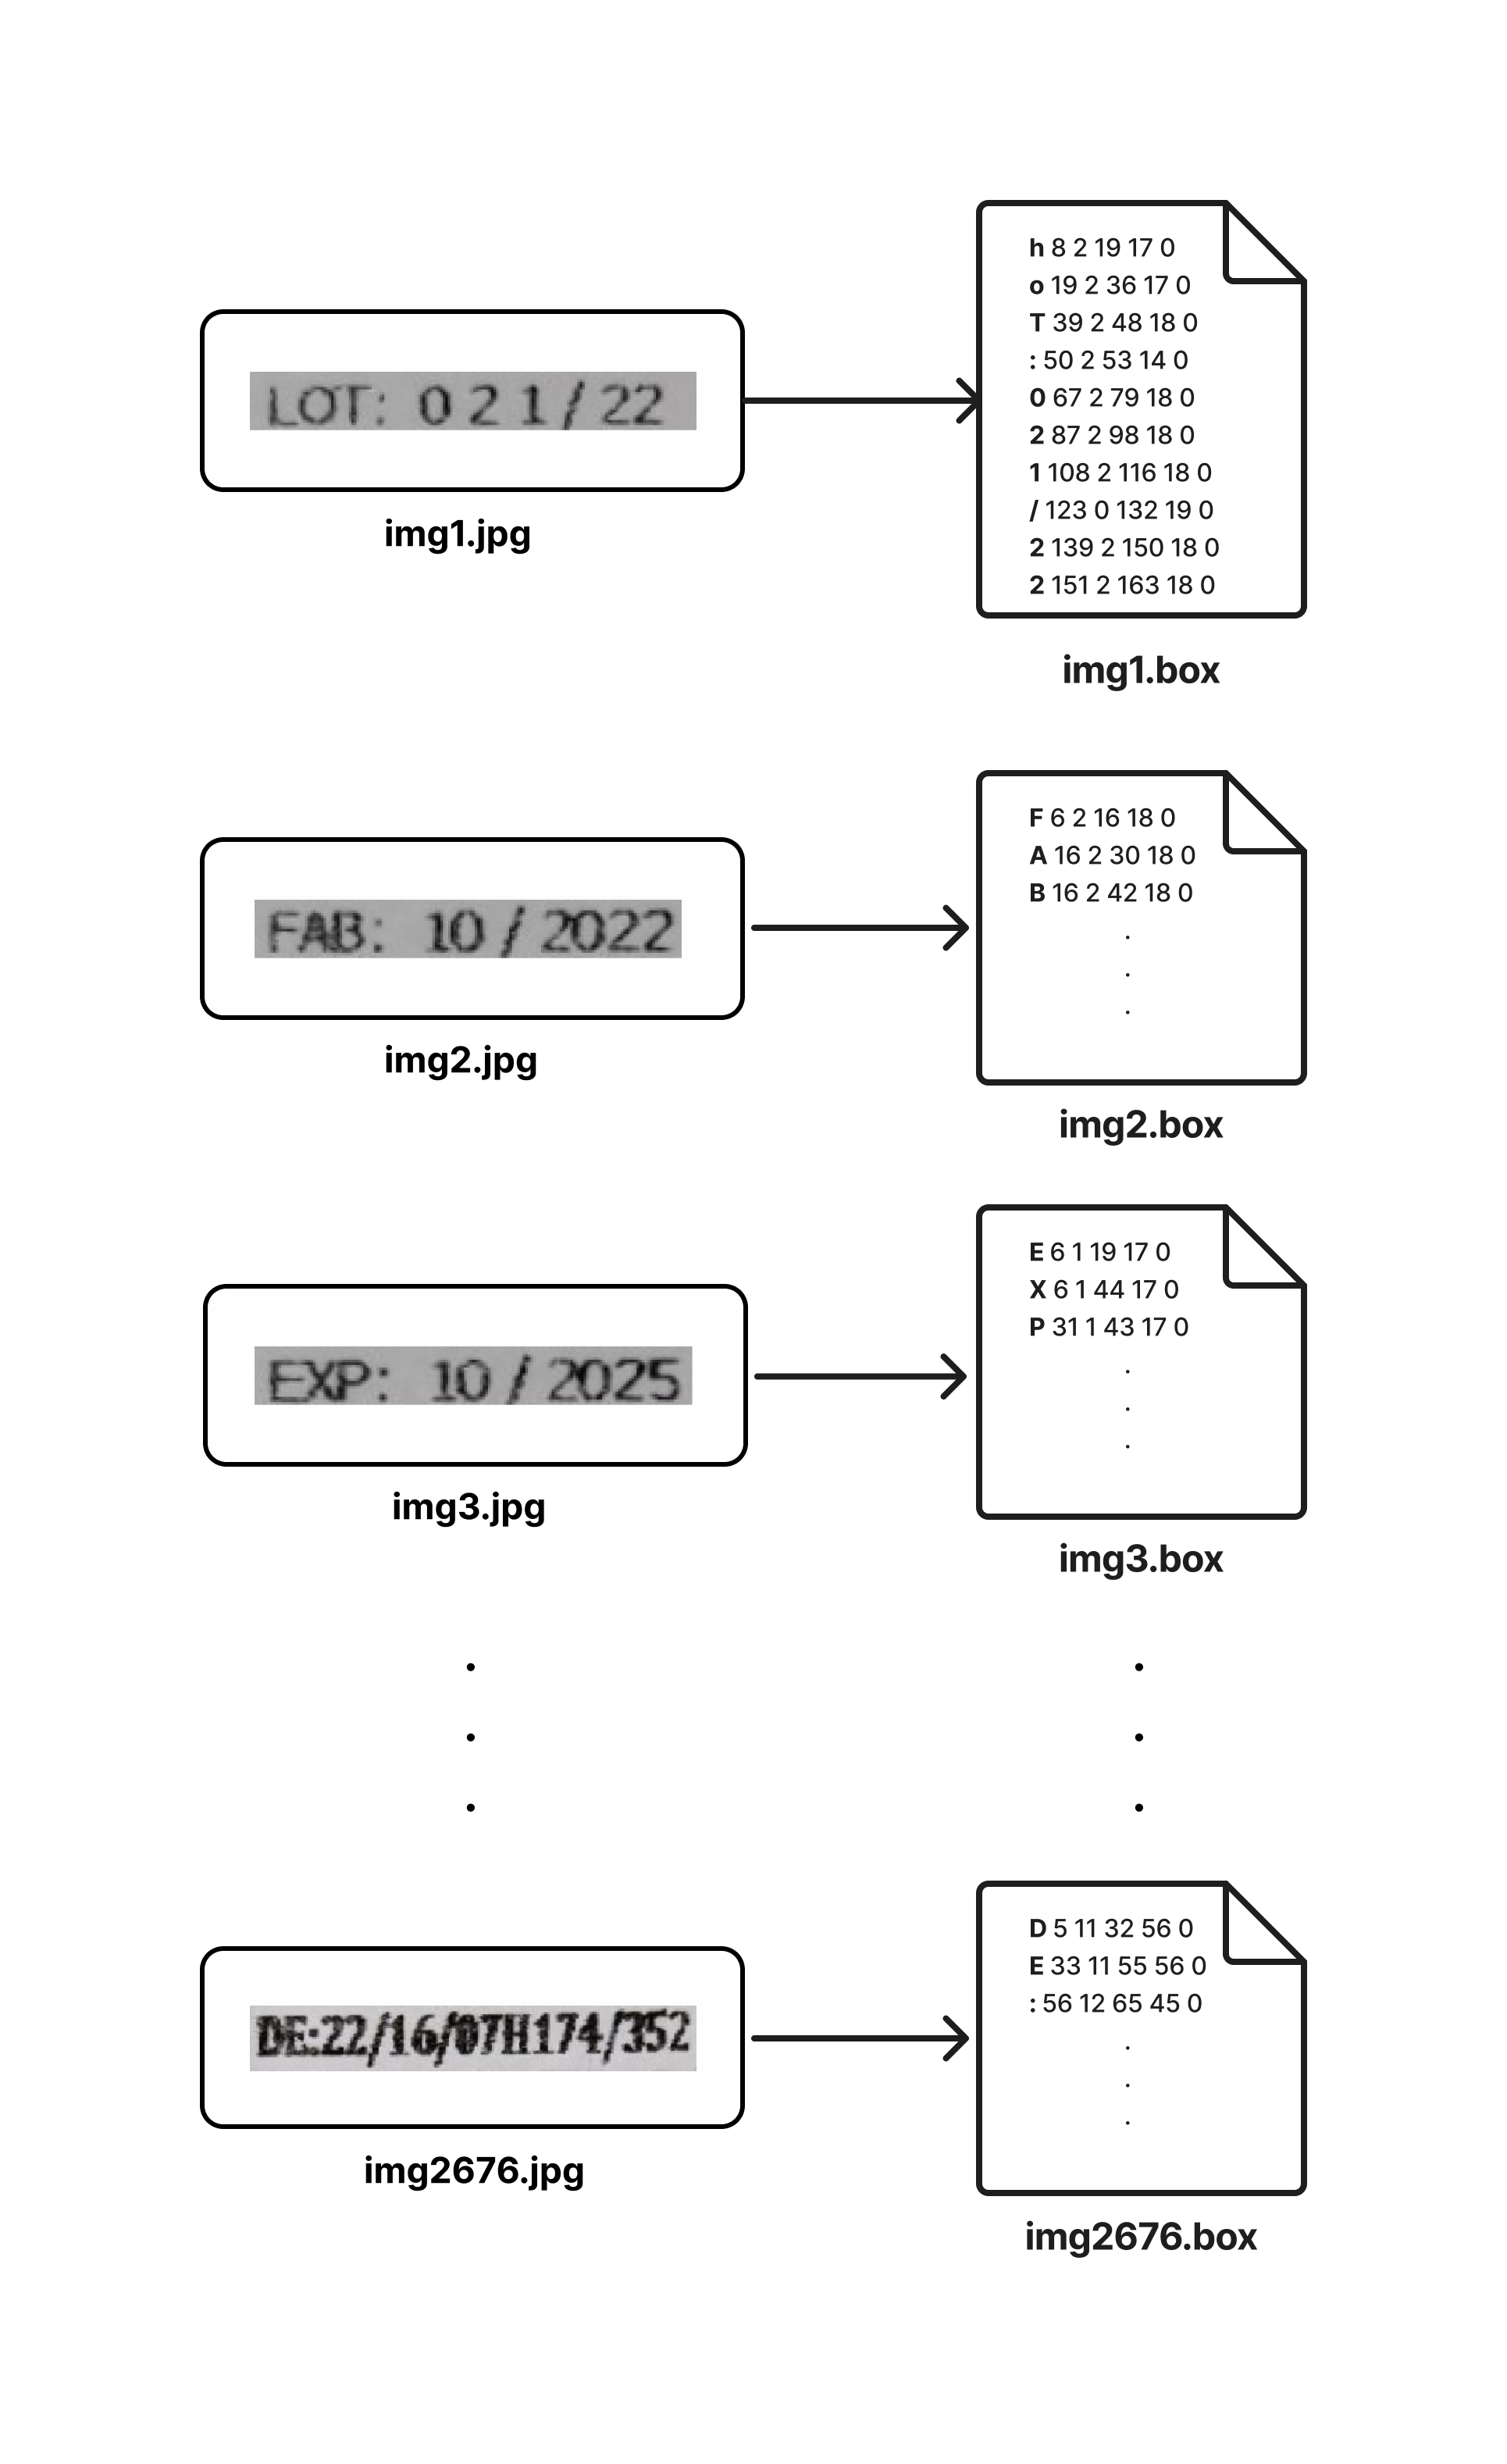
\includegraphics[width=0.5\textwidth]{Figures/Chapter 3/Box_File_Creation.png}
\caption{Box File Creation Process}
\label{fig:boxfilecreation}
\end{figure}
%\end{comment}

The lines of text and their corresponding box files are then compiled into .lstm files using Tesseract’s training tools. As illustrated in Figure \ref{fig:lstmfilecreation}, each image and its associated box file are processed together to produce an .lstm file (e.g., \texttt{img1.lstm}). This file contains the feature representations used during model training.
%\begin{comment}
    

\begin{figure}[H]
\centering
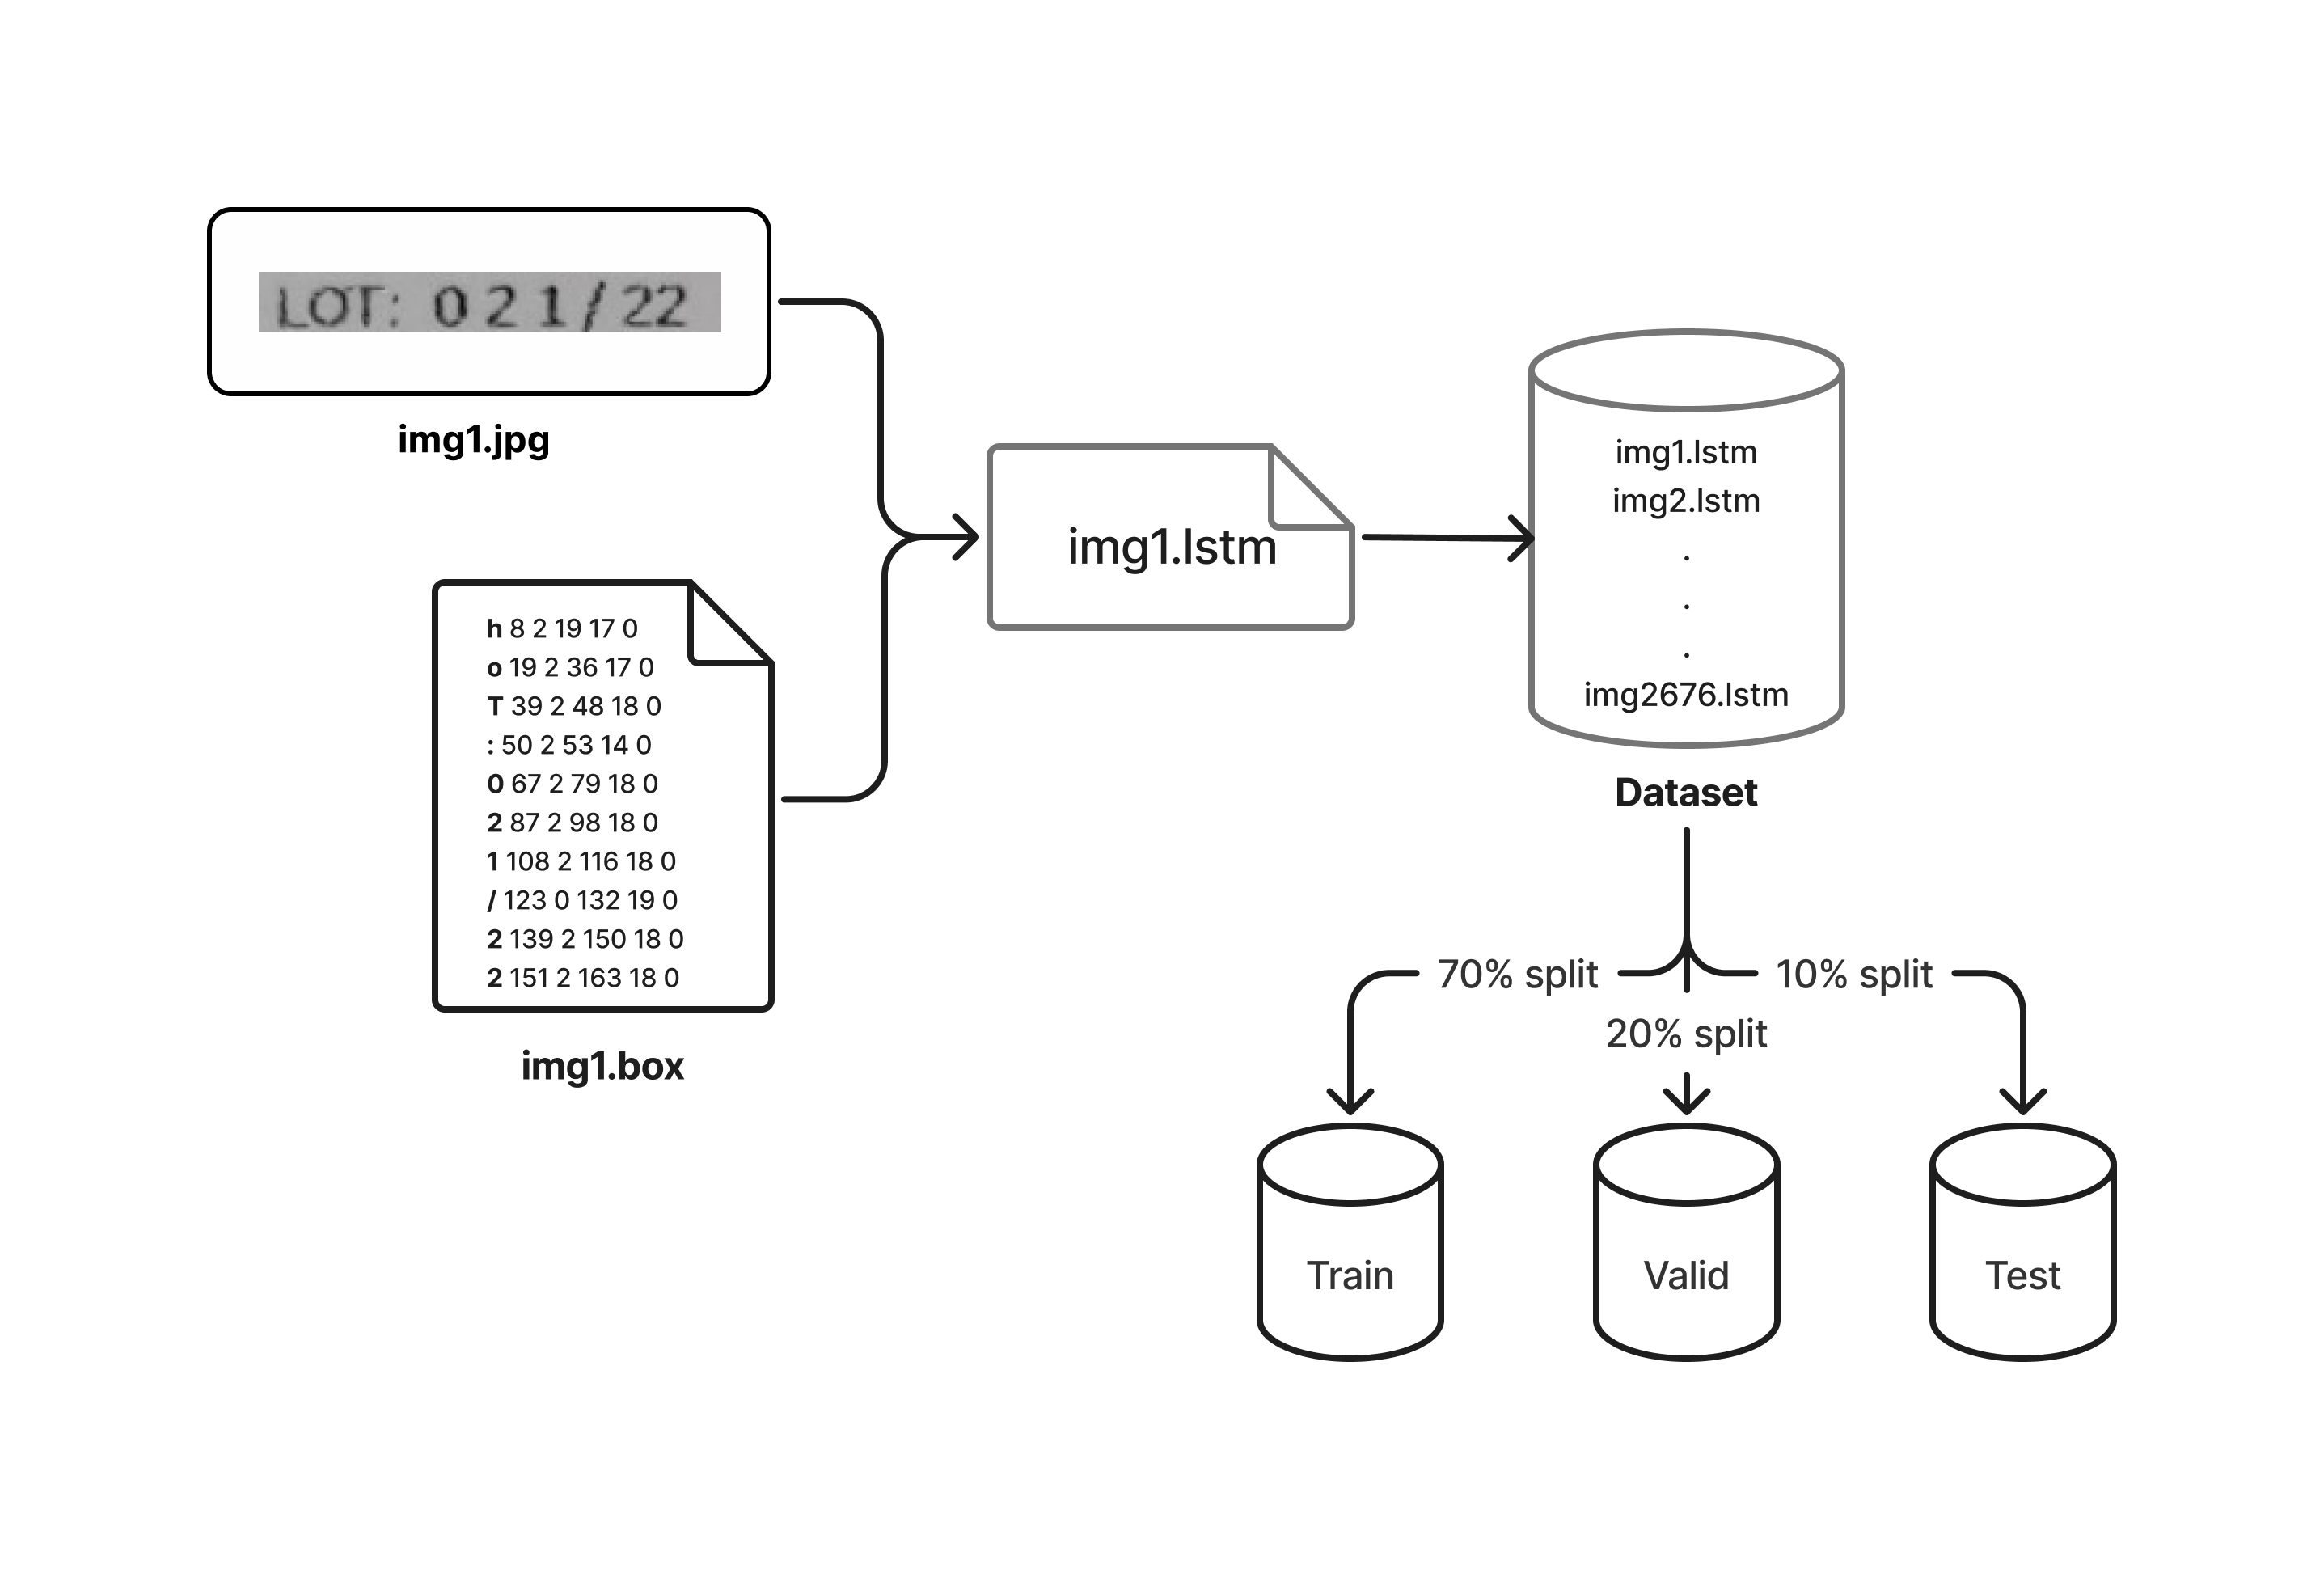
\includegraphics[width=\textwidth]{Figures/Chapter 3/Lstm_File_Creation.png}
\caption{LSTM File Creation and Dataset Splitting}
\label{fig:lstmfilecreation}
\end{figure}

%\end{comment}
The complete set of .lstm files is collected to form the dataset, which is then divided into training, validation, and testing subsets. A standard 70\%-20\%-10\% split is used to ensure balanced and representative samples across all phases of model development. 

\subsubsection{Standard Tesseract}

Pretrained OCR models, while powerful, are typically trained on generic datasets that may not reflect domain-specific or regional language characteristics. In the case of Algerian medical labels, this discrepancy becomes especially problematic. The pretrained OCR models we implemented were not exposed to the visual or linguistic patterns specific to Algerian Medical Labels—such as unique font styles, multi-language text (Arabic/French), abbreviations, or specialized medical terms. As a result, applying the model without adaptation leads to poor recognition performance.

\begin{figure}[H]
\centering
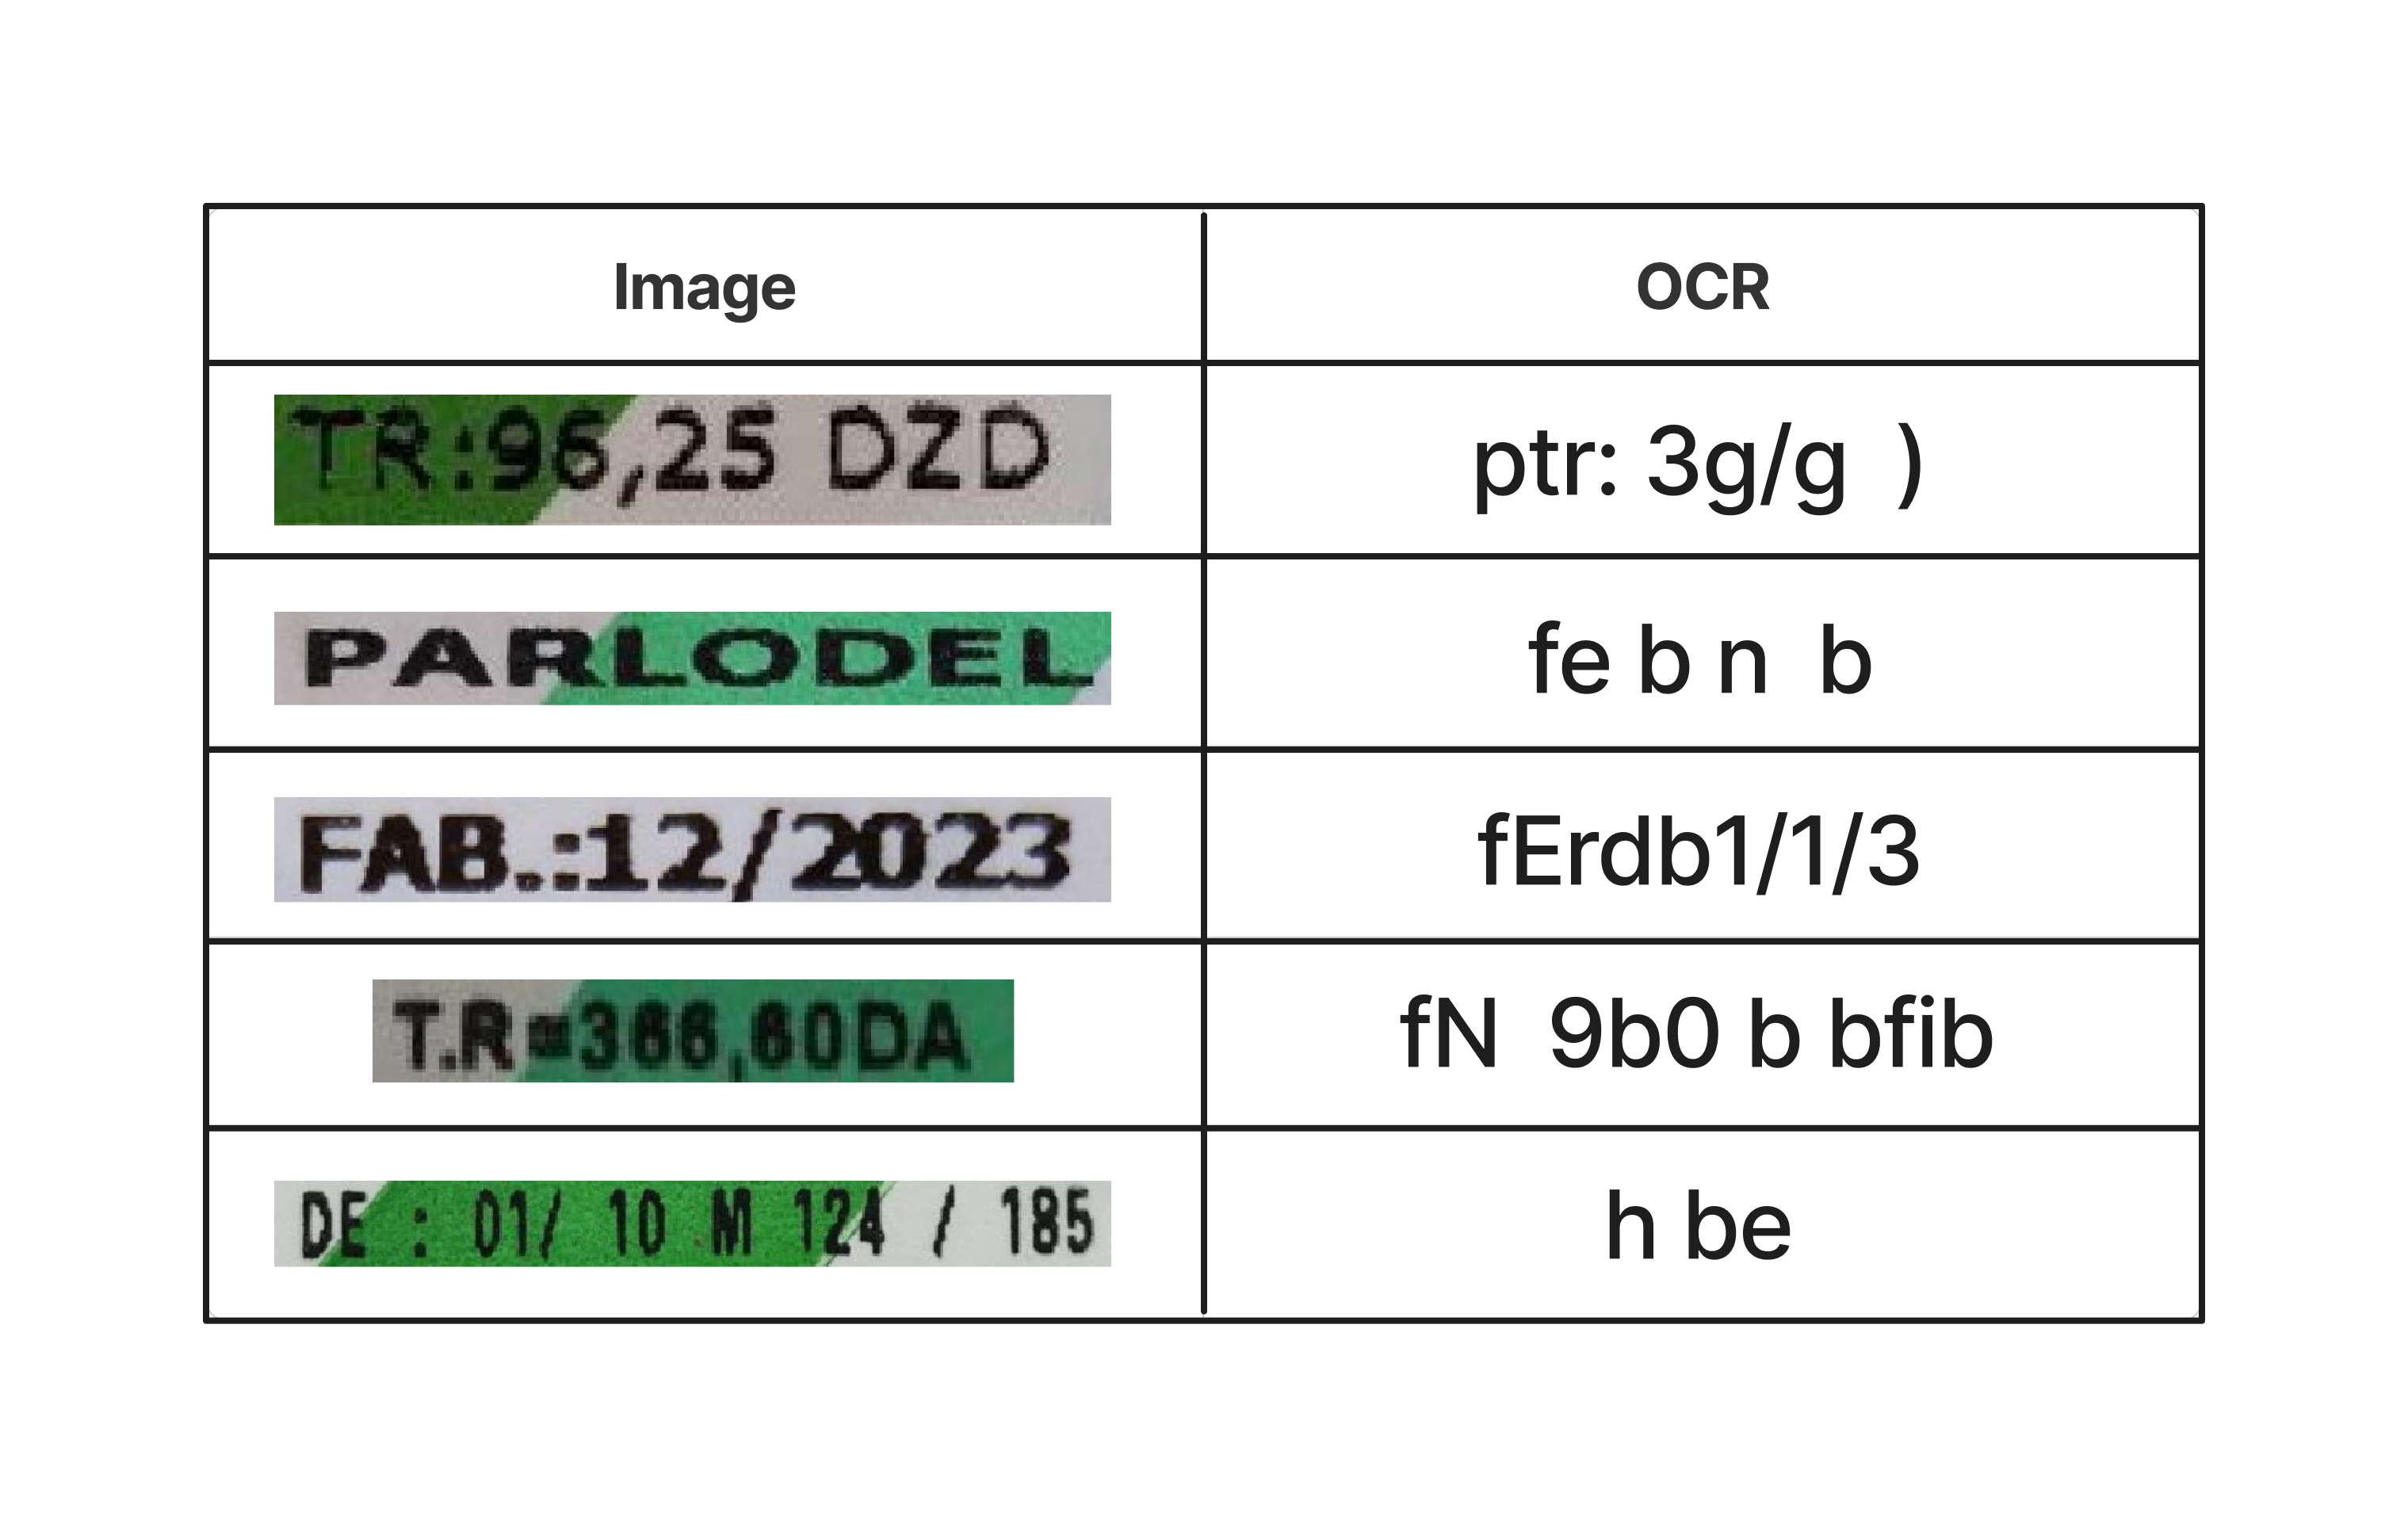
\includegraphics[width=0.75\textwidth]{Figures/Chapter 3/standard_tesseract_results.png}
\caption{Tesseract OCR on a test sample}
\label{fig:tesseractocrtestsample}
\end{figure}

The Table \ref{fig:tesseractocrtestsample} demonstrates the Standard Tesseract OCR results on some samples from our Testing Set. The results clearly demonstrate the low accuracy of the standard Tesseract due to the lack of domain adaptation and training on data representative of Algerian medical labels. These limitations highlight the necessity of fine-tuning or retraining the model with domain-specific data to improve recognition performance in this context.
 

\subsubsection{Fine-Tuned Tesseract}

\subsubsection*{Tesseract Fine-Tuning Process}

Using the training dataset obtained, as illustrated in Figure \ref{fig:lstmfilecreation}, Tesseract can be fine-tuned to produce a domain-adapted OCR model. This process begins by preparing a large number of \texttt{.lstm} files, which are then used alongside the base language model weights file \texttt{fra.traineddata}\footnote{\url{https://github.com/tesseract-ocr/tessdata}} (French language, since the medical labels are in French) to adapt the model to specific fonts, styles, or scanning conditions.

\begin{figure}[H]
\centering
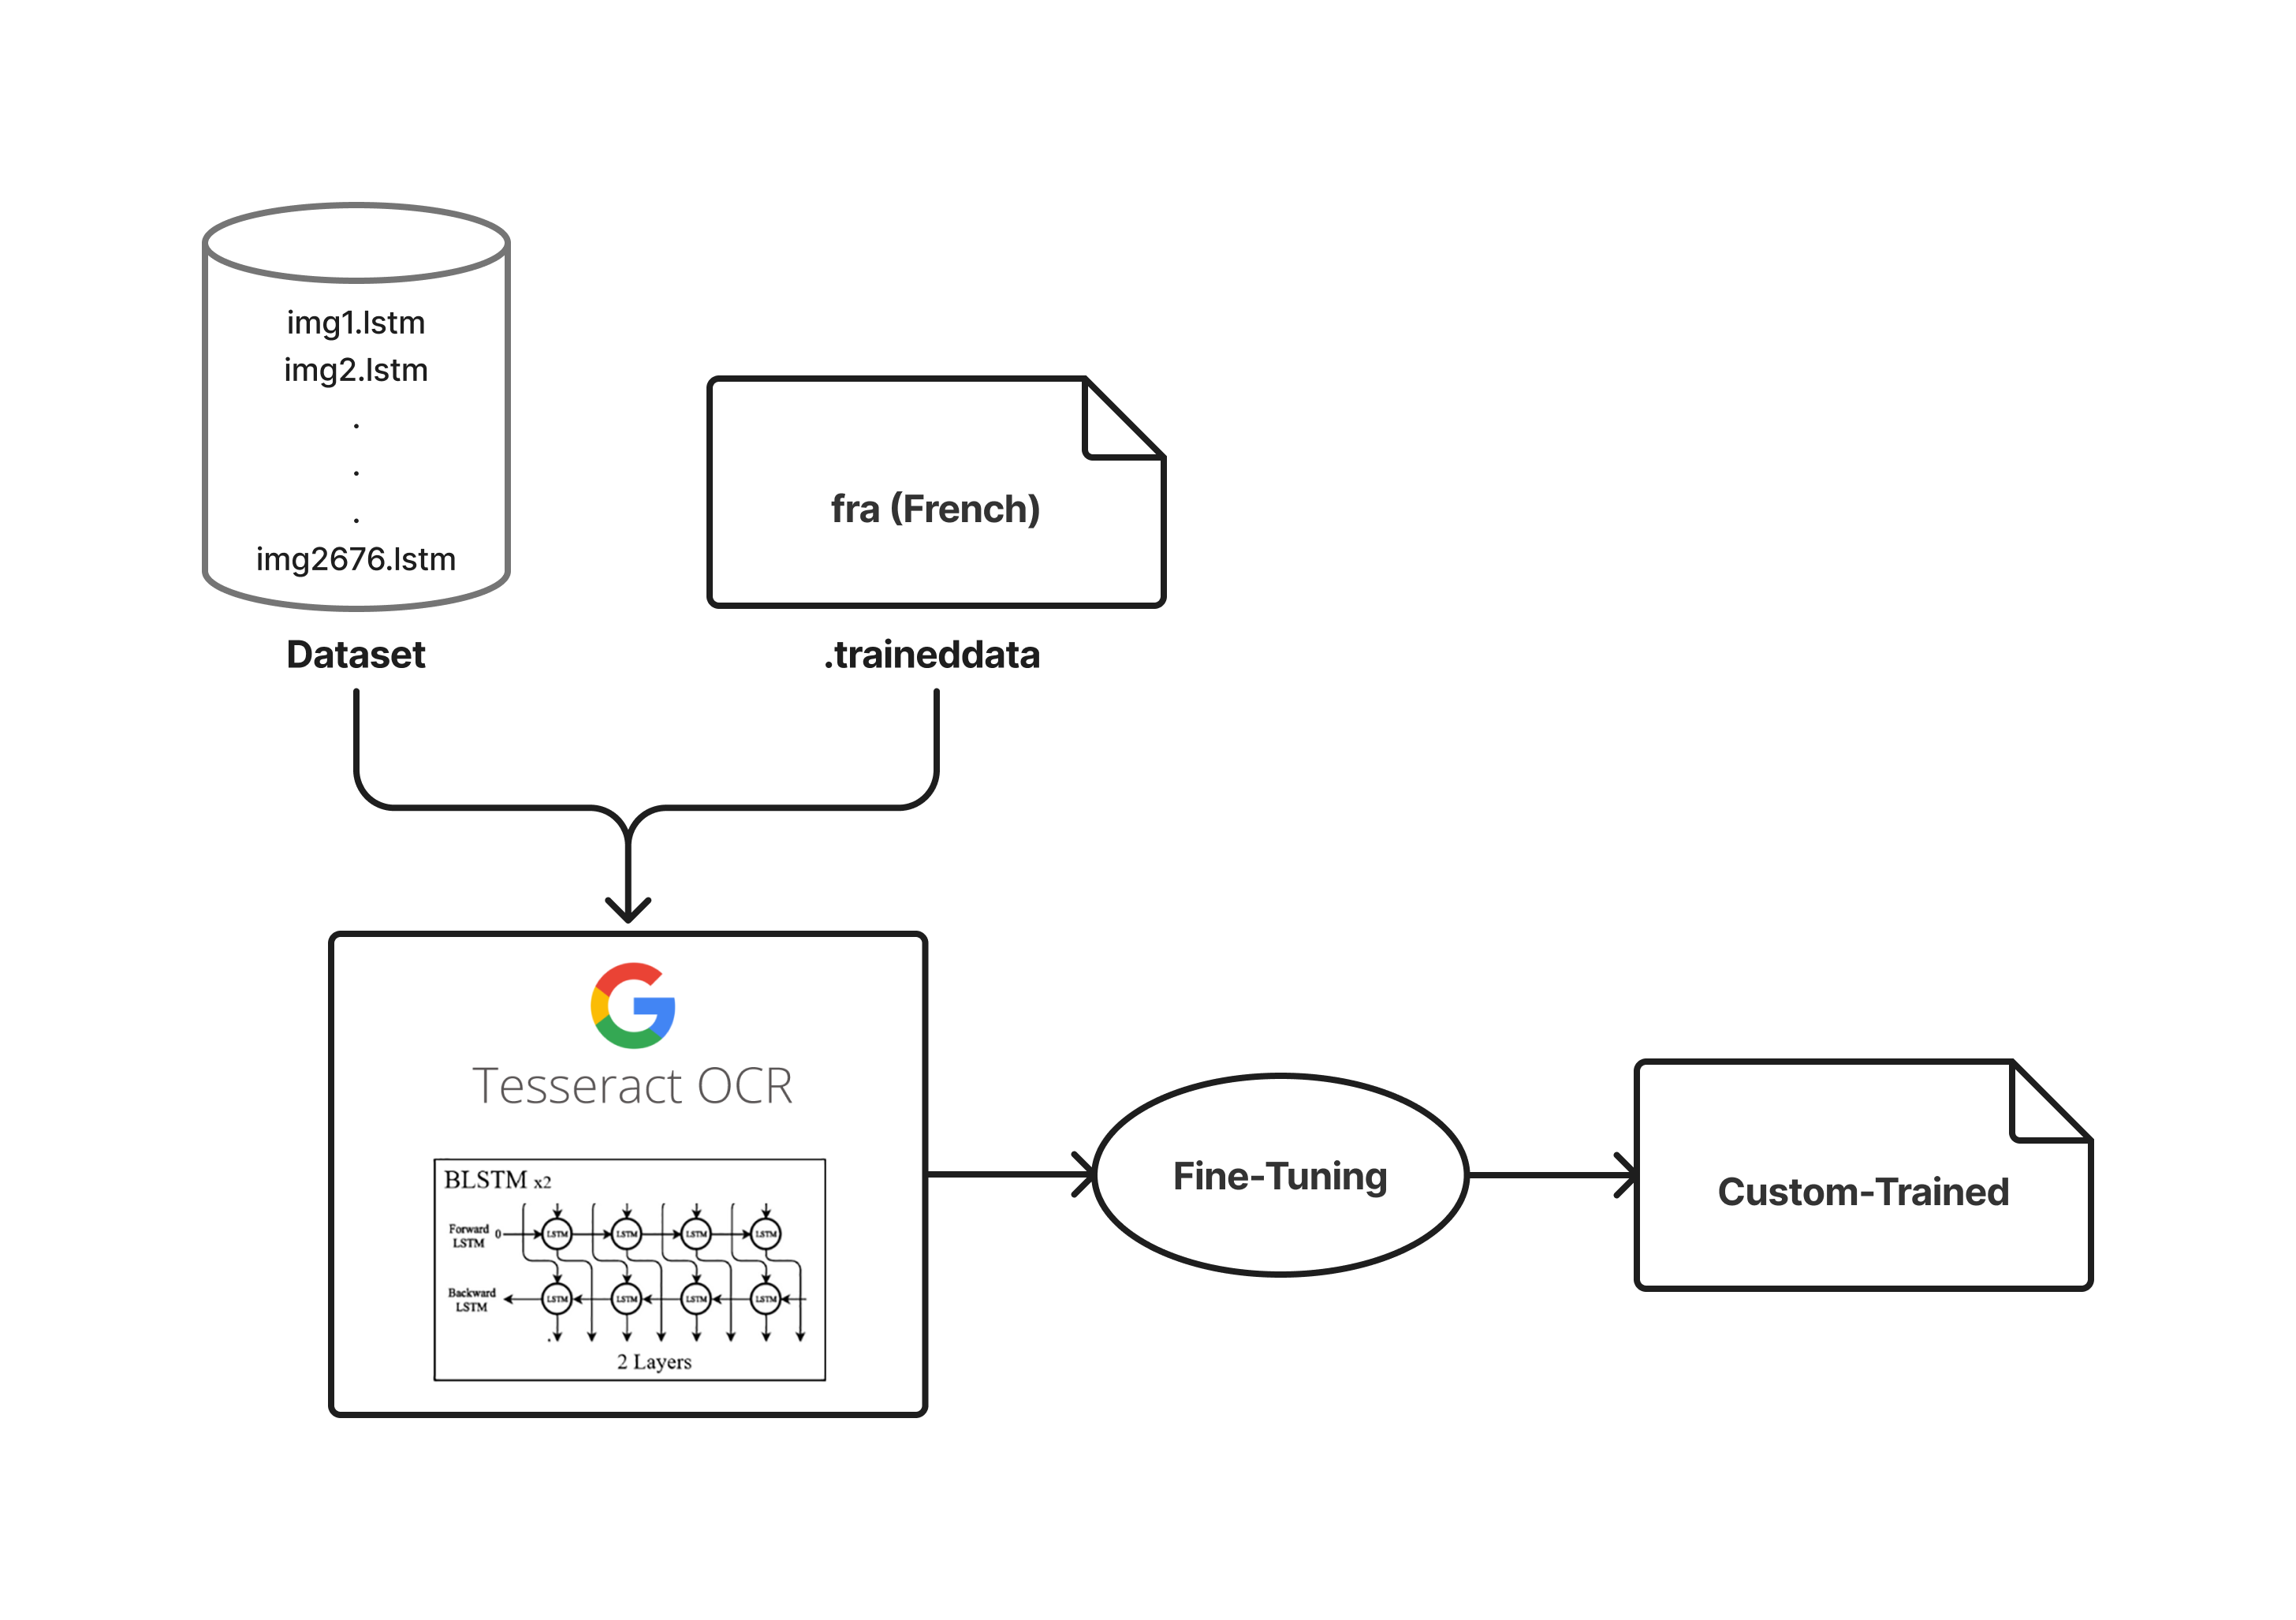
\includegraphics[width=\textwidth]{Figures/Chapter 3/Tesseract_Fine_Tuning_Process.png}
\caption{Tesseract Fine-Tuning Process}
\label{fig:tesseractfinetuning}
\end{figure}

As shown in Figure \ref{fig:tesseractfinetuning}, the fine-tuning process involves feeding both the dataset and a \texttt{.traineddata} file into the Tesseract OCR engine. This engine, based on a bidirectional LSTM (BLSTM x2) architecture, adjusts its internal parameters to the characteristics of the new dataset. The model weights are updated iteratively through multiple training steps, minimizing recognition errors on the custom data.

After fine-tuning, the output is a custom \texttt{.traineddata} file containing updated model weights better suited to the medical label domain, typography, and document format. This custom model enables higher OCR accuracy on similar documents, surpassing the standard pretrained Tesseract model.

\subsubsection*{Fine-Tuning Results}

To evaluate fine-tuning performance, we tracked training and validation losses over multiple iterations. Additionally, Character Error Rate (CER) was calculated at each checkpoint to monitor recognition accuracy progression.

Since the PyTesseract package downloaded from the official Tesseract website\footnote{\url{https://tesseract-ocr.github.io/}} does not include validation scripts or built-in evaluation tools, we developed a custom validation procedure. After each checkpoint, the fine-tuned model was saved and evaluated on the validation set to detect overfitting and assess training progress.

\vspace{0.5cm}

\begin{figure}[H]
\centering
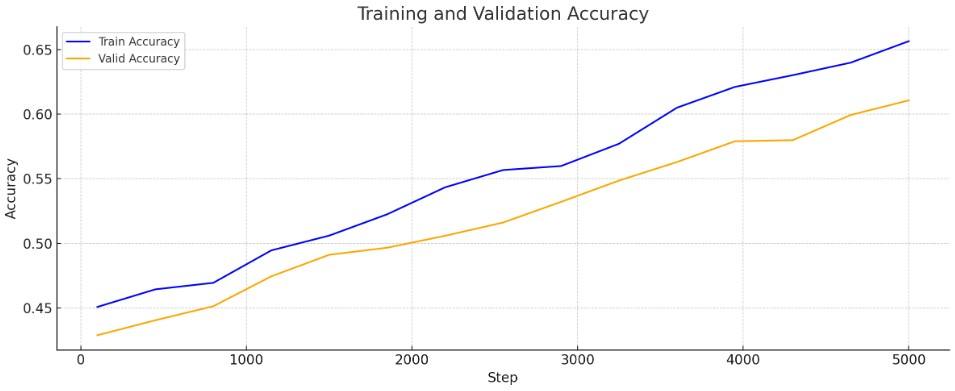
\includegraphics[width=0.90\linewidth]{Figures/Chapter 3/Tessearct_validation_training.jpg}
\caption{Training and Validation Loss During Tesseract Fine-Tuning}
\label{fig:tesseract-loss-curve}
\end{figure}

\vspace{0.5cm}

\begin{figure}[H]
\centering
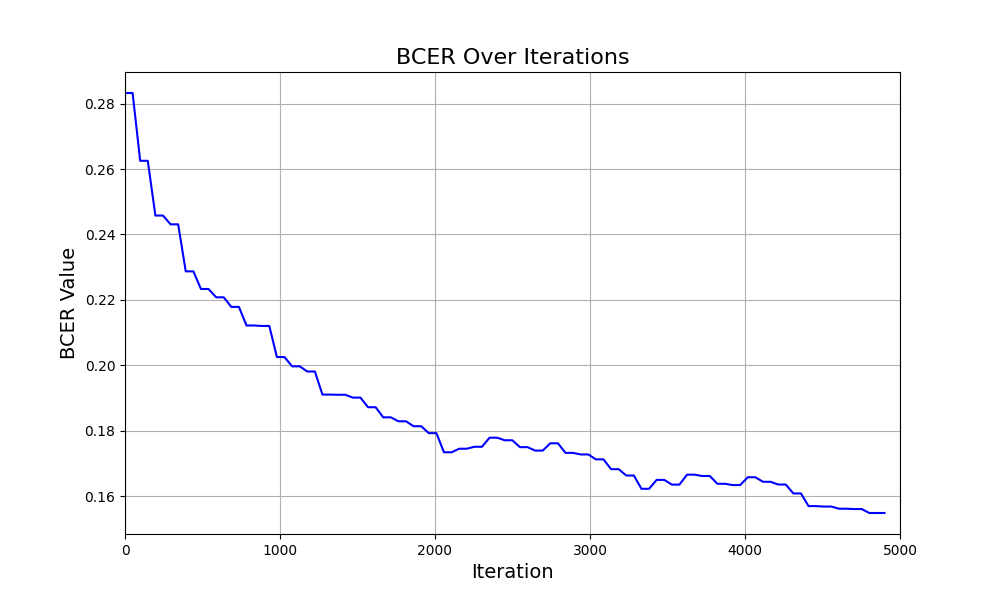
\includegraphics[width=0.90\linewidth]{Figures/Chapter 3/Tesseract_Fine_Tune_CER.png}
\caption{Character Error Rate (CER) Over Iterations During Tesseract Fine-Tuning}
\label{fig:tesseract-cer-curve}
\end{figure}

Figure \ref{fig:tesseract-loss-curve} depicts the evolution of training and validation losses during fine-tuning. Both losses gradually decreased, indicating that the model was learning to generalize well. The training loss dropped from a high initial value to a significantly lower final value, while the validation loss followed a similar downward trend with a relatively small gap, suggesting minimal overfitting.

Figure \ref{fig:tesseract-cer-curve} shows the Character Error Rate (CER) over training iterations. Initially, the CER was high (approximately 0.28), but it steadily declined to about 0.155 by the end of training. The smooth decrease indicates stable training without major fluctuations or overfitting.

The CER was computed using the following formula:

\begin{equation}
\text{CER} = \frac{\sum_{i=1}^{N} \text{EditDistance}(\text{prediction}_i, \text{ground\_truth}_i)}{\sum_{i=1}^{N} \text{Length}(\text{ground\_truth}_i)}
\end{equation}

where \textit{EditDistance} represents the Levenshtein distance between the predicted string and the ground truth. This metric calculates the minimum number of single-character insertions, deletions, or substitutions required to transform one string into the other. A lower CER value indicates better recognition accuracy.


\subsubsection{Standard vs. Fine-Tuned Tesseract Comparison}

Fine-tuning the Tesseract OCR engine on domain-specific data addresses the limitations of the standard pretrained model, which is not adapted to the unique characteristics of Algerian medical labels. Training on custom-labeled data reflecting local fonts, languages, and formatting conventions enables the model to better interpret the content accurately.

This domain adaptation leads to a significant improvement in recognition performance, as demonstrated by the substantial reduction in Character Error Rate (CER) when comparing the standard and fine-tuned models on the test set.

\vspace{0.5cm}
\begin{table}[H]
\caption{ Standard vs Fine-Tuned CER comparison on Tesseract Models}
\centering
\begin{tabular}{lc}
\hline
\textbf{Model Version} & \textbf{CER } \\
\hline
Standard Tesseract & 0.8824 \\
Fine-Tuned Tesseract & 0.3142 \\
\hline
\end{tabular}

\label{tab:Tesseract-cer-comparison}
\end{table}

\vspace{0.5cm}
\begin{table}[H]
\caption{Sample Predictions: Standard vs. Fine-Tuned Tesseract}
\centering
\begin{tabular}{llll}
\hline
\textbf{Image} & \textbf{Ground Truth} & \textbf{Fine-Tuned Prediction} & \textbf{Standard Prediction} \\
\hline
img871.jpg & DE: 039/13B 010/17 & DE: 039/138 010/17 & pee: 39/13 m /17 \\
img1530.jpg & LOT: 24092 & LOT: 20092 & fo: 4n34 \\
img868.jpg & Céfalexine & Cefalexine & vigF1gji \\
img546.jpg & PYOSTACINE®500 mg & PYOSTACINE & pvgtrine \\
img456.jpg & PPA:1287.50+2,50 & PPA:1 287.50+2.50 & "ippI:1 401 g) \\
\hline
\end{tabular}

\label{tab:tesseract-sample-predictions}
\end{table}

Table \ref{tab:Tesseract-cer-comparison} quantitatively compares the Character Error Rate (CER) between the standard pretrained Tesseract and the fine-tuned model on the medical label dataset. The fine-tuned model reduced the CER from 0.8824 to 0.3142, representing a 64.4\% improvement.

Table \ref{tab:tesseract-sample-predictions} provides qualitative examples of predictions from both models compared with ground truth. The fine-tuned model consistently produces outputs closer to the true text, while the standard model frequently generates distorted or incorrect characters, illustrating its inability to handle the specialized dataset effectively.

This fine-tuning approach outperformed previous work \cite{ait2024automated}, thanks to an expanded dataset, the addition of a validation step, and improved manual annotation and labeling.


\subsection{Model 2 - EasyOCR -: Description and Experimental Results}

Modern OCR engines such as EasyOCR employ a Convolutional Recurrent Neural Network (CRNN) backbone, which unifies spatial feature extraction with sequence modeling and end‐to‐end transcription. 


\begin{figure}[H]
    \centering
    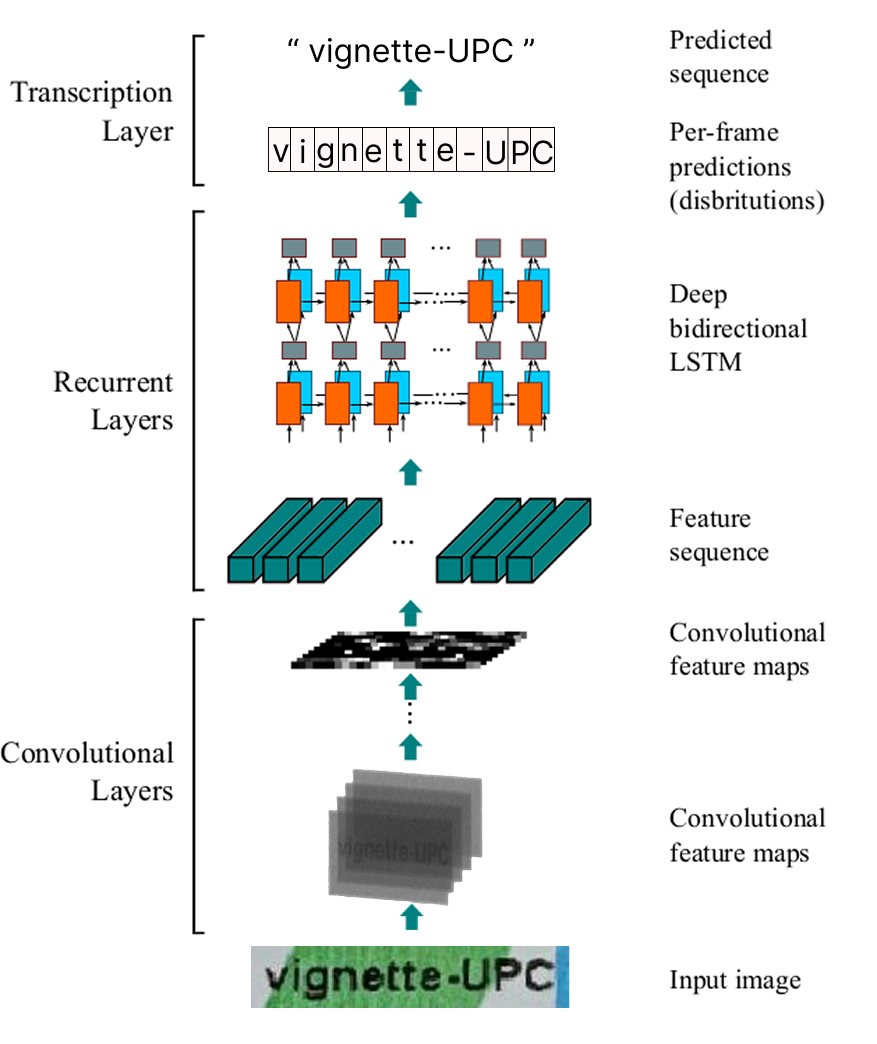
\includegraphics[width=0.8\textwidth]{Figures/Chapter 3/EasyOCR_Architecture.png}
    \caption{EasyOCR Architecture}
    \label{fig:EasyOCRArchitecture}
\end{figure}



In our implementation, the CRNN is organized into three logical stages:

\subsubsection*{Convolutional Feature Extraction}
The first stage is a stack of 2D convolutional layers (e.g.\ VGG or ResNet blocks) interleaved with pooling operations. Given an input image of a text line, these layers learn to detect low‑level cues (edges, corners) and higher‑level patterns (strokes, character shapes). By progressively reducing the spatial height (while preserving sufficient width), the network produces a set of high‑dimensional \emph{feature maps} whose columns correspond to spatial “slices” of the original image.

\subsubsection*{Sequence Modeling}
Next, the 2D feature maps are reshaped into a 1D sequence of feature vectors: each time‑step vector is obtained by taking the channels at a given horizontal position. This sequence feeds into one or more bidirectional Long Short‑Term Memory (BiLSTM) layers. The BiLSTM processes the data both left‑to‑right and right‑to‑left, enabling the model to capture contextual dependencies across neighboring characters. This context is crucial for disambiguating visually similar glyphs (for instance, “I” vs. “l”) based on their surroundings.

\subsubsection*{Transcription with CTC}
Finally, each time‑step hidden state is passed through a small fully‑connected layer and softmax to yield a probability distribution over the character alphabet plus a special “blank” symbol. We then apply Connectionist Temporal Classification (CTC) decoding: repeated symbols are collapsed and blanks removed, producing the final predicted string. CTC allows training directly on image–text pairs without requiring explicit character‐level bounding boxes.

Overall, this CRNN + CTC pipeline elegantly bridges the gap between raw pixels and text sequences, learning implicit alignments during training and delivering robust recognition across a variety of fonts, layouts, and image conditions.

\subsubsection{Dataset Configuration}
EasyOCR requires two separate CSV files as input: one for training and the other for validation or testing. For this work, the dataset was divided using an 70\%–20\%-10\% split, with approximately 2,080 image-label pairs allocated for training and 20\% of 460 for validation and the remaining 10\% for testing.

Each CSV file consists of two columns. The first column, \textbf{filename}, contains the name of the image file (e.g., \texttt{img1.jpg}, \texttt{img2.jpg}), while the second column, \textbf{words}, holds the ground truth transcription of the text present in the corresponding image. These CSV files serve as the main input format for the EasyOCR training pipeline.

It is important to note that the image files and their corresponding text labels must be located in the same directory as the CSV files. The EasyOCR model uses the paths defined in the CSVs to locate and process the data during training and evaluation.

\begin{figure}[H]
    \centering
    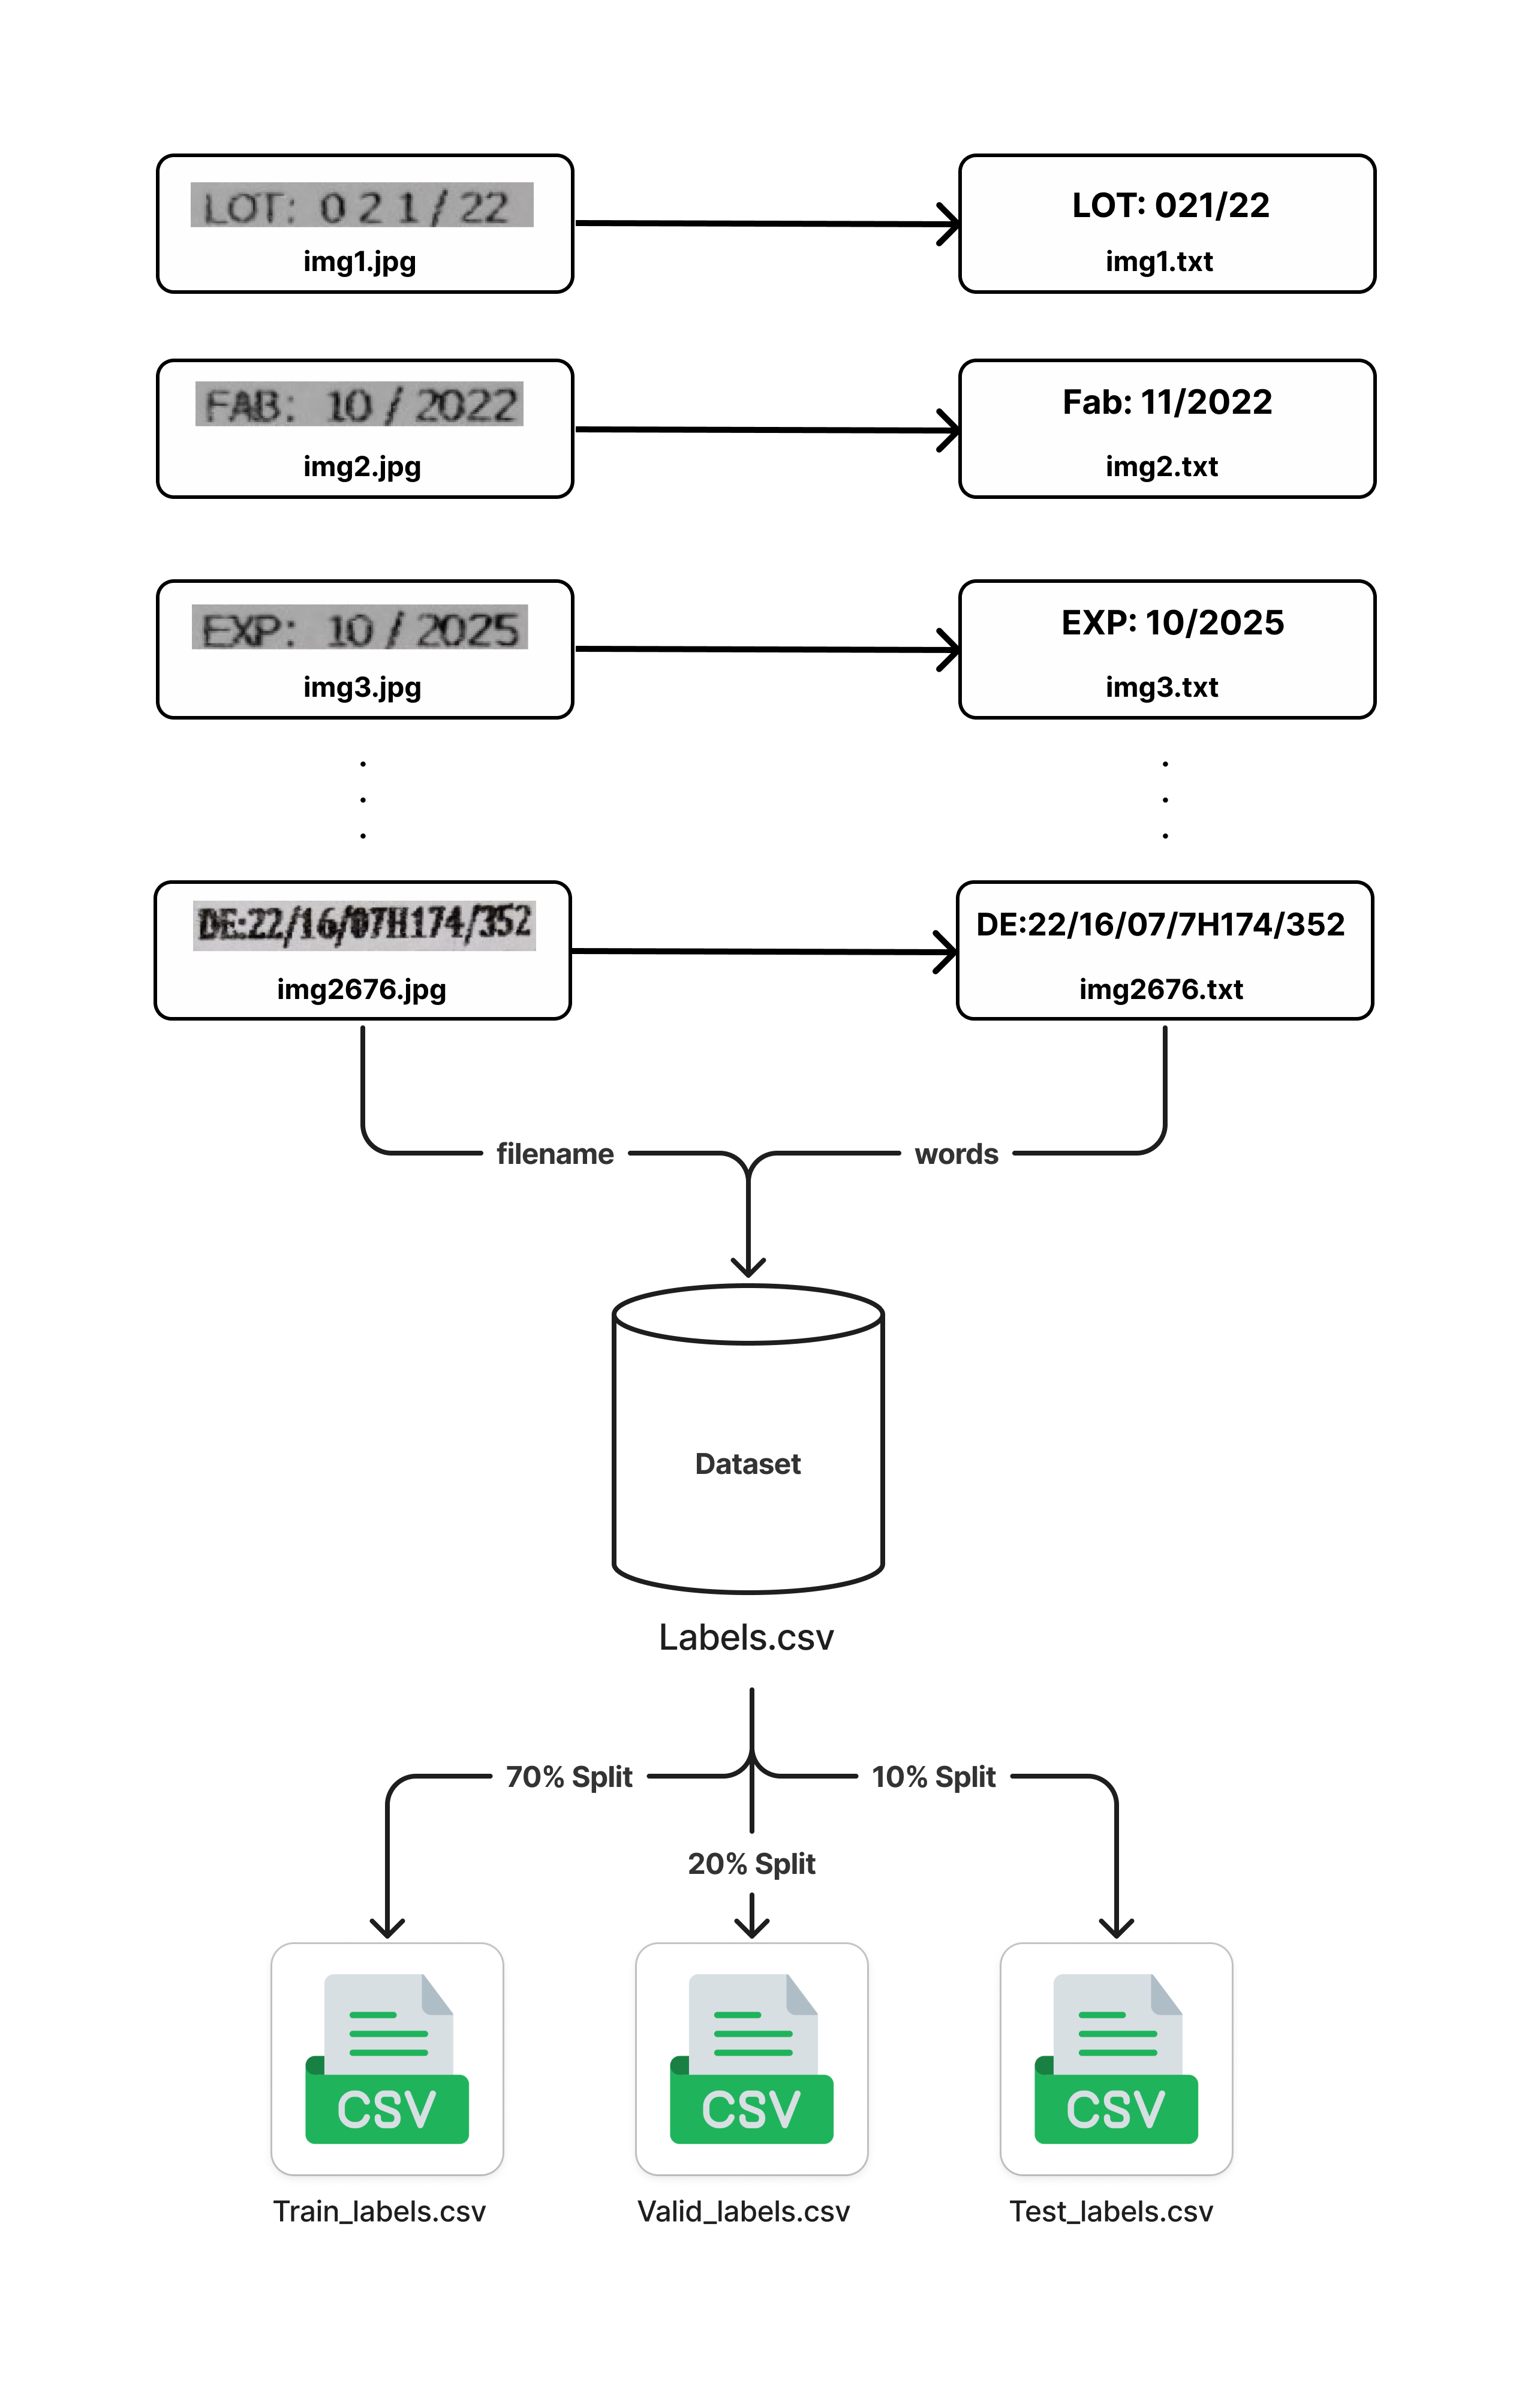
\includegraphics[width=0.57\textwidth]{Figures/Chapter 3/easyocr_dataset.png}
    \caption{EasyOCR Dataset Configuration}
    \label{fig:easyocrdatasetConfiguration}
\end{figure}


\subsubsection{Standard EasyOCR}

Although EasyOCR uses a Convolutional Recurrent Neural Network, sometimes it struggles with low-resolution text, complex backgrounds, or mixed-language content commonly found on Algerian medical labels.

\begin{figure}[H]
\centering
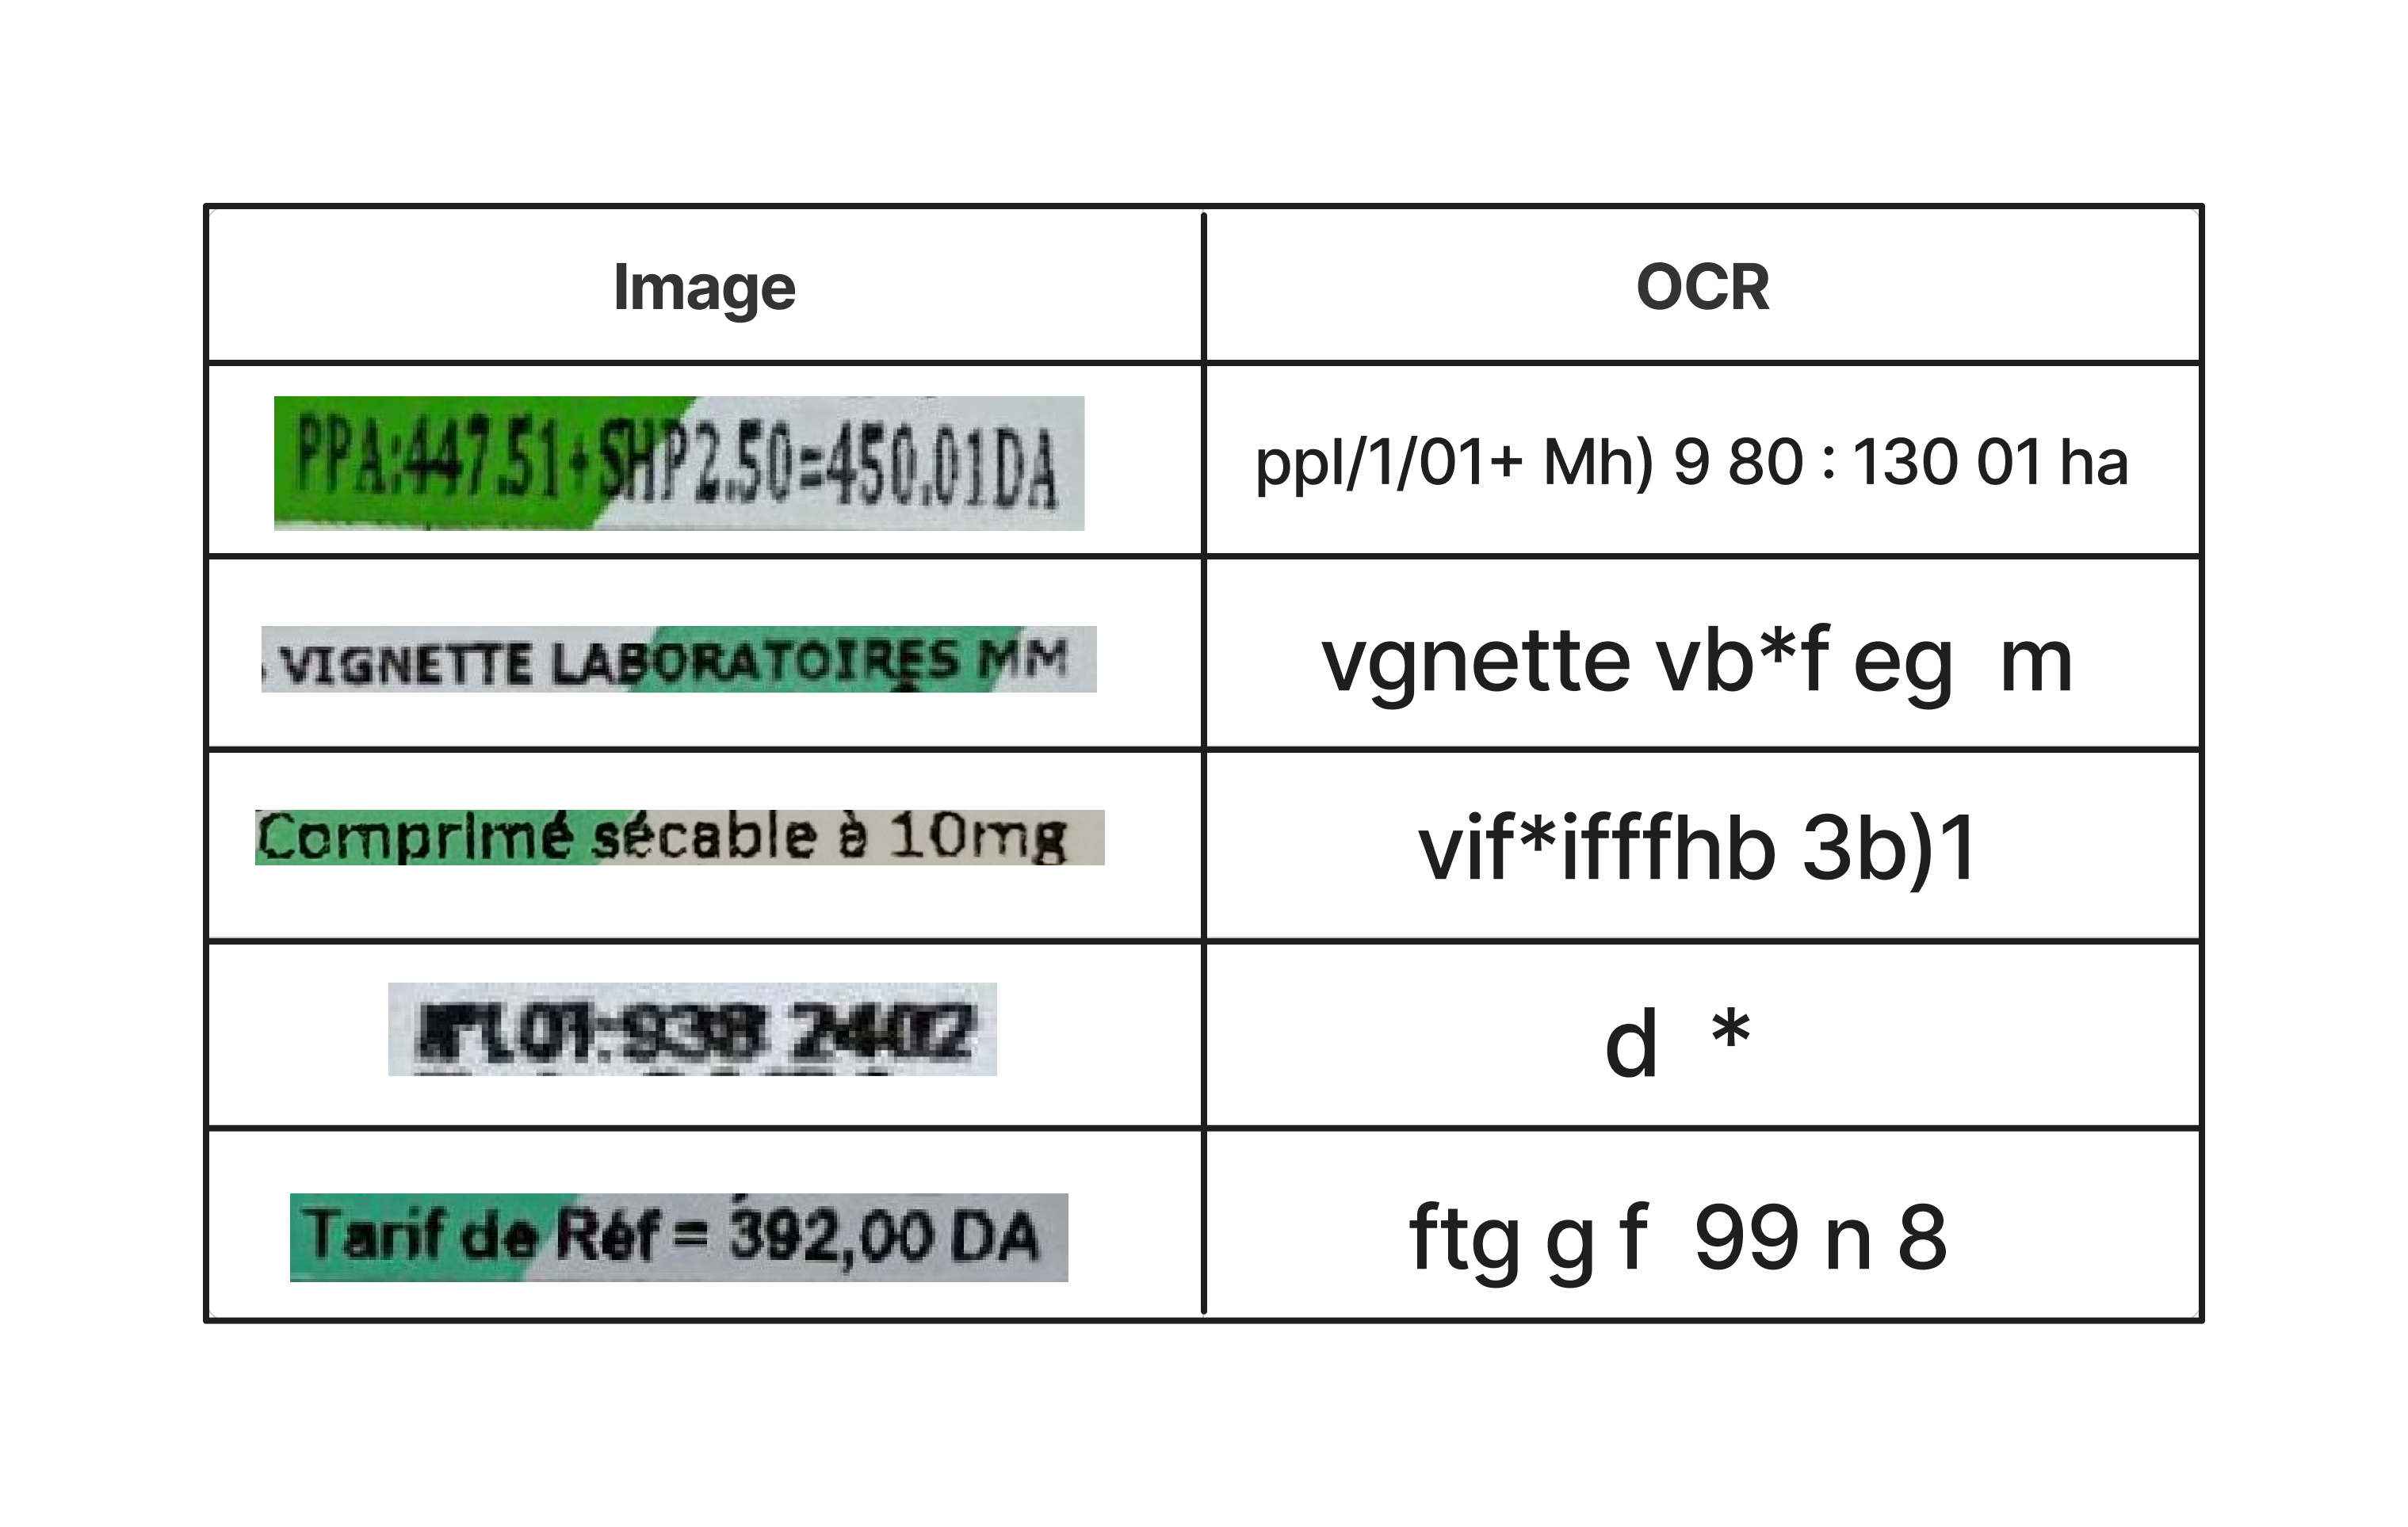
\includegraphics[width=0.75\textwidth]{Figures/Chapter 3/standard_easyocr_results.png}
\caption{EasyOCR on a test sample}
\label{fig:standardeasyocrresults}
\end{figure}

The table \ref{fig:standardeasyocrresults} demonstrates the Standard EasyOCR results on some samples from our Testing Set. The results clearly demonstrate the low accuracy of the standard Tesseract due to the lack of adaptation to the specific features of Algerian medical labels. Many characters were misread or omitted, especially in cases involving small fonts, mixed languages (Arabic and French), or uncommon abbreviations. This highlights the need for fine-tuning or custom models tailored to this type of domain-specific data.


\subsubsection{Fine-Tuned EasyOCR}
\subsubsection*{YAML Configuration}

EasyOCR uses a YAML configuration file to centralize key parameters controlling data loading, model architecture, and the training process.

\begin{figure}[H]
    \centering
    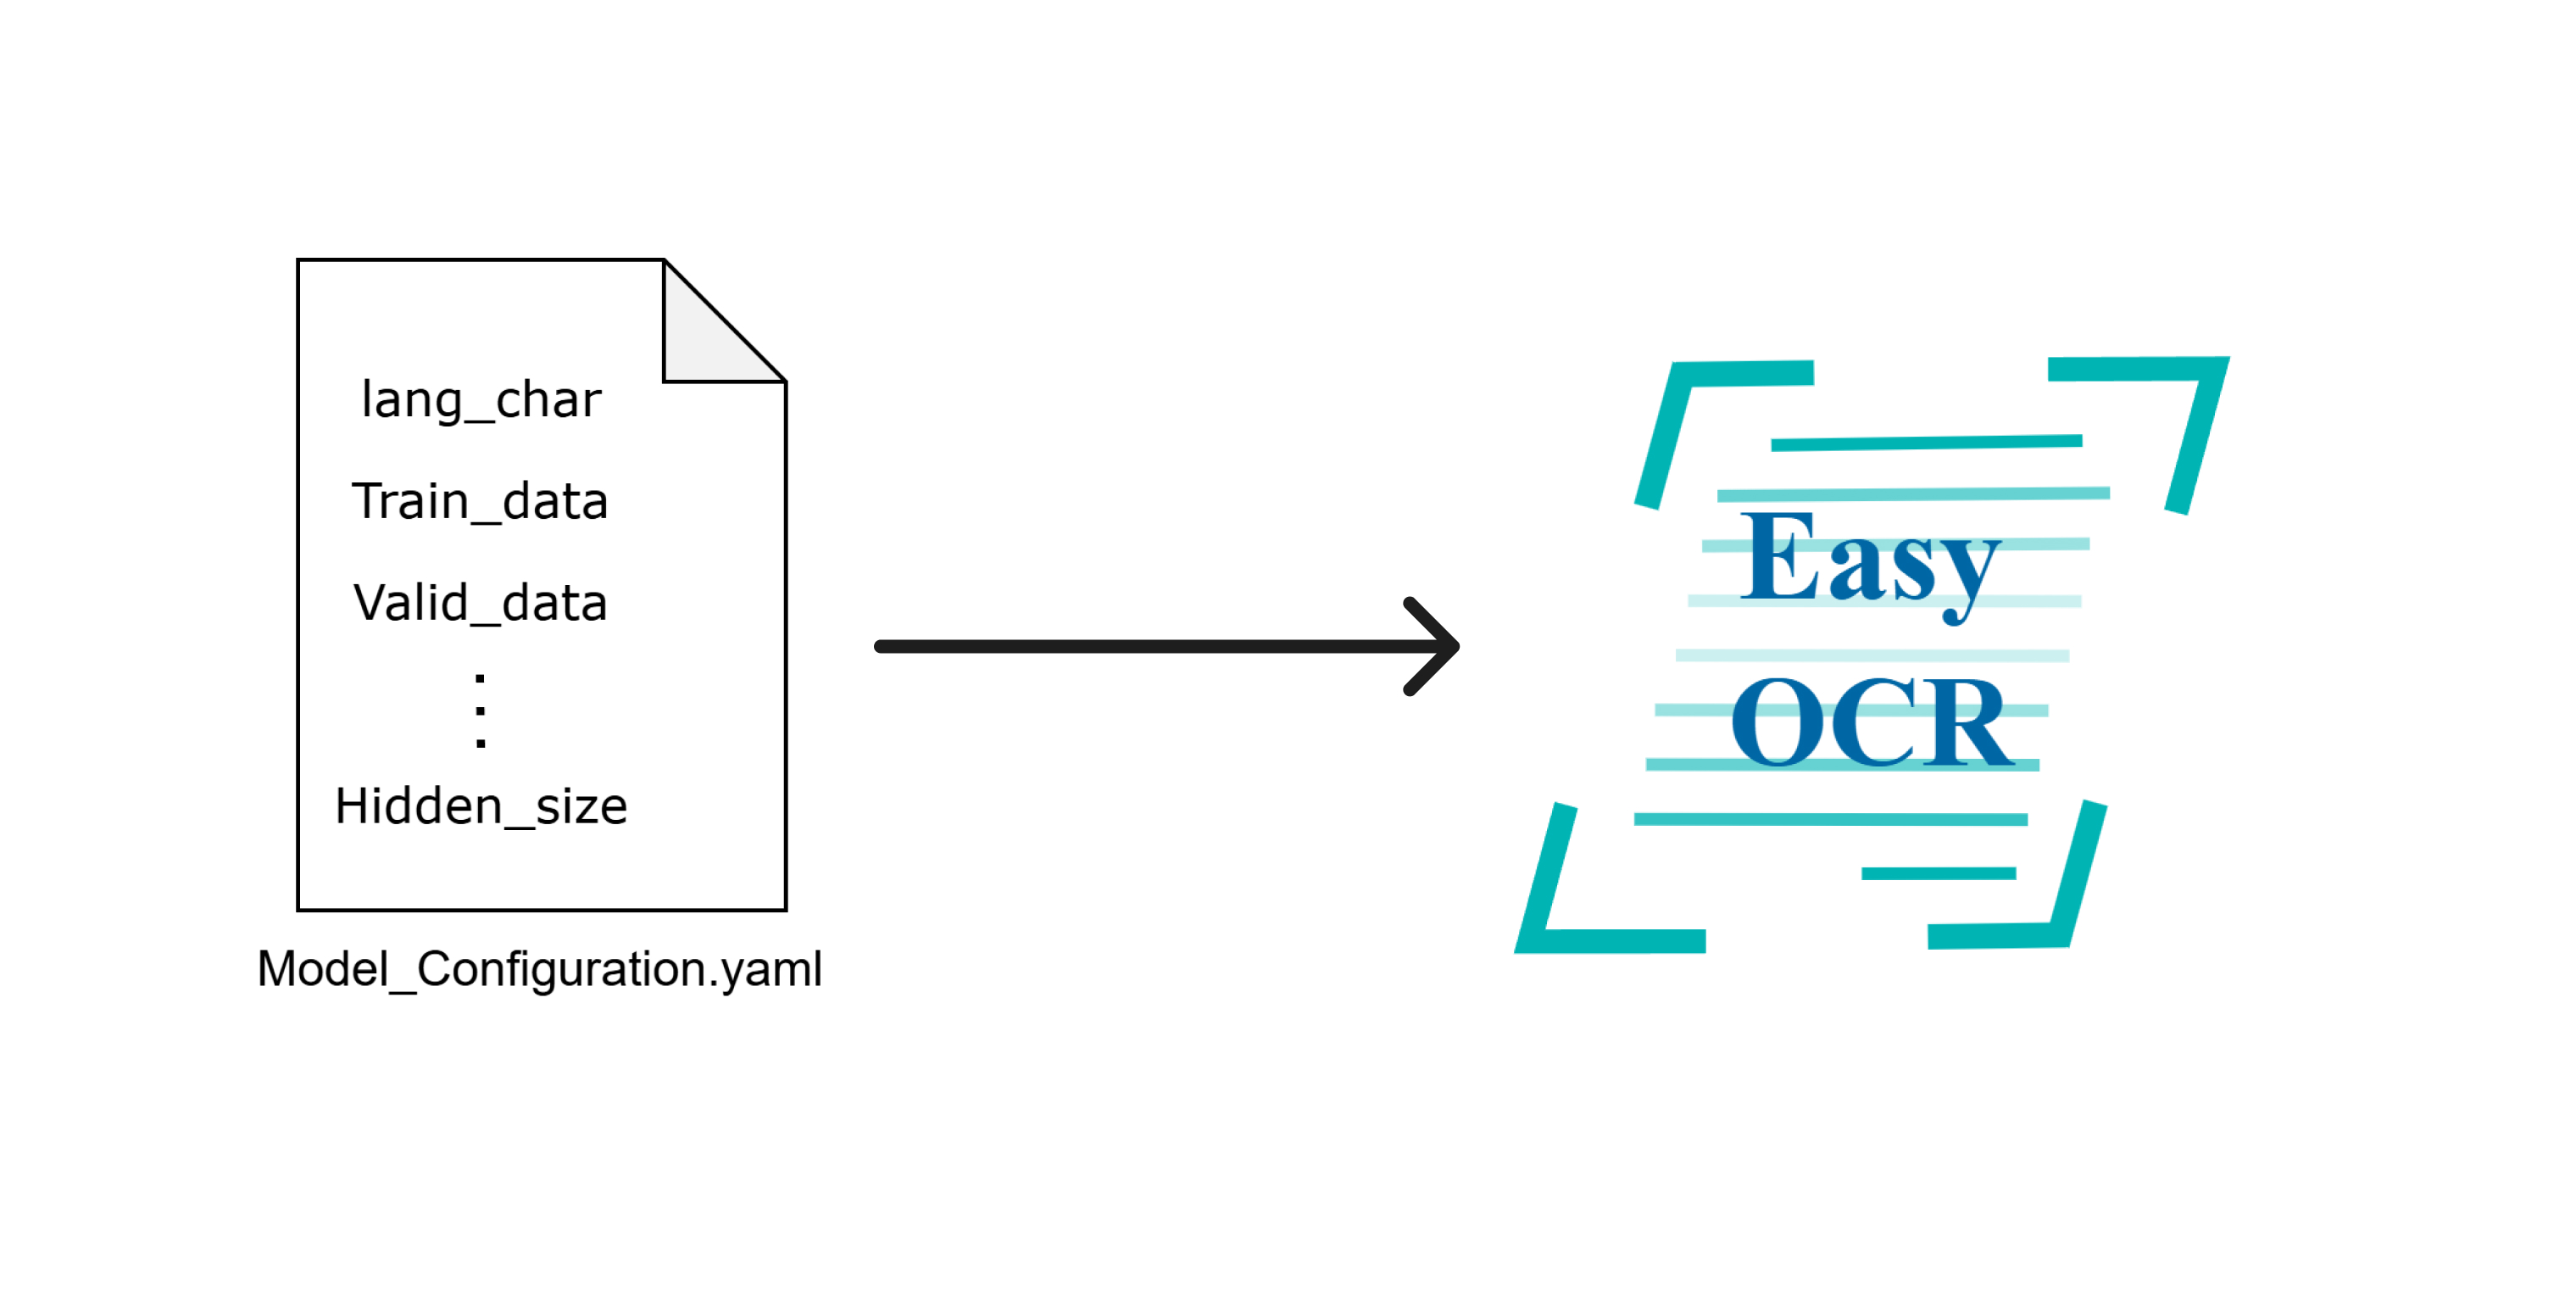
\includegraphics[width=0.80\textwidth]{Figures/Chapter 3/YAML_Configuration.jpg}
    \caption{YAML file configuration}
    \label{fig:YAMLConfiguration}
\end{figure}

Below are some parameters from our example YAML, with a brief explanation:

\begin{itemize}
  \item \textbf{number}: Defines numeric characters (e.g., 0--9) that the model predicts.
  \item \textbf{lang\_char}: Specifies the alphabetic character set (A--Z, a--z) for recognition.
  \item \textbf{train\_data}, \textbf{valid\_data}: Paths to training and validation image folders (with labels).
  \item \textbf{batch\_size}: Number of samples per iteration during training.
  \item \textbf{num\_iter}: Total optimizer update steps to run.
  \item \textbf{valInterval}: Frequency (in iterations) to evaluate on validation data.
  \item \textbf{saved\_model}: Filepath to load/save model checkpoints.
  \item \textbf{imgH}, \textbf{imgW}: Target height and width (pixels) for input resizing.
  \item \textbf{Transformation}: Geometric correction method (e.g., TPS) for text alignment.
  \item \textbf{FeatureExtraction}: Backbone CNN choice (e.g., VGG, ResNet) to extract features.
  \item \textbf{SequenceModeling}: Contextual encoder (e.g., BiLSTM) capturing sequential dependencies.
  \item \textbf{Prediction}: Decoding head (CTC or attention) generating final text outputs.
  \item \textbf{input\_channel}: Number of image channels (1=grayscale, 3=RGB).
  \item \textbf{output\_channel}: Channel dimension of CNN feature maps.
  \item \textbf{hidden\_size}: Size of hidden states in the sequence modeling layer.
\end{itemize}


\subsubsection*{Fine-Tuning Results}

To evaluate the effectiveness of the fine-tuning process, the model’s training and validation losses were monitored over multiple epochs. In addition, the Character Error Rate (CER) was calculated after each epoch to track the improvement in recognition accuracy.


\vspace{0.5cm}
\begin{figure}[H]
\centering
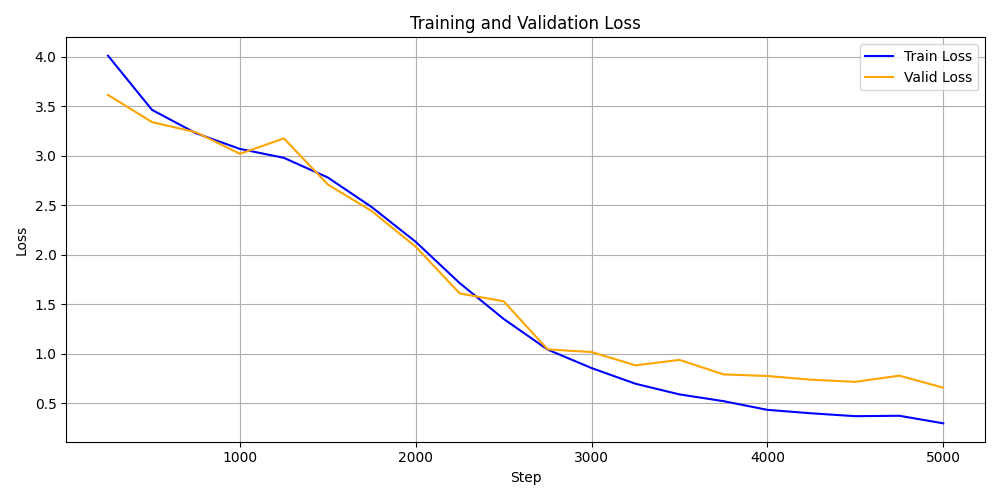
\includegraphics[width=0.75\linewidth]{Figures/Chapter 3/easyocr_validtrain_loss.png}
\caption{Training and Validation Loss During EasyOCR Fine-Tuning}
\label{fig:easyocr-loss-curve}
\end{figure}

\begin{figure}[H]
\centering
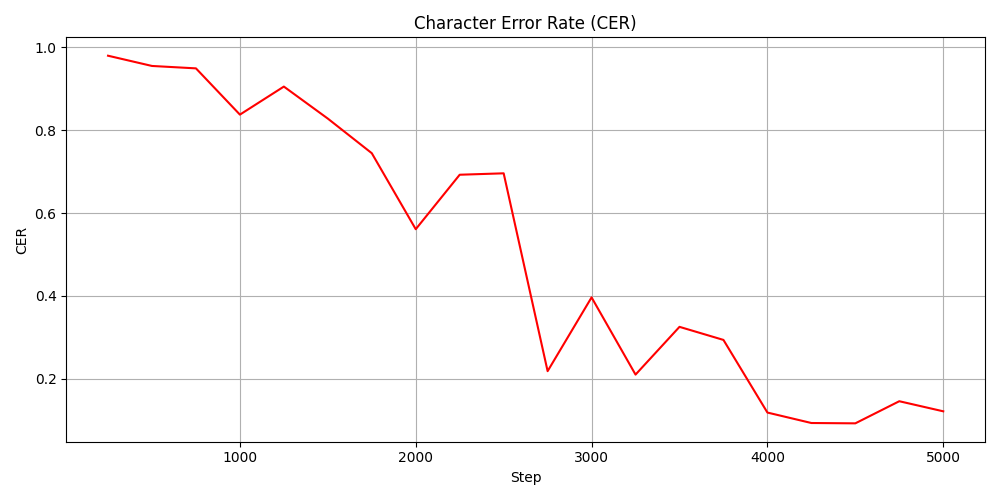
\includegraphics[width=0.75\linewidth]{Figures/Chapter 3/easyocr_cer.png}
\caption{Character Error Rate (CER) Over Iterations During EasyOCR Fine-Tuning}
\label{fig:easyocr-cer-curve}
\end{figure}

Figure~\ref{fig:easyocr-loss-curve} illustrates the training and validation loss curves during fine-tuning. The training loss steadily decreased, while the validation loss stabilized after several iterations, indicating effective learning without significant overfitting.

Figure~\ref{fig:easyocr-cer-curve} shows the Character Error Rate (CER) over the course of training. A sharp decrease in CER occurs during the initial iterations, followed by gradual improvements, demonstrating that the model adapted well to the Algerian medical label dataset.

\subsubsection{Standard vs. Fine-Tuned EasyOCR Comparison}

Fine-tuning the EasyOCR model on a domain-specific dataset addresses some of the limitations of the standard pretrained version, which is not trained for specialized tasks like recognizing Algerian medical labels. By retraining the model using images and text extracted from this specific context, it becomes more familiar with the visual patterns, terminology, and formatting typically found on local pharmaceutical packaging. As a result, the model demonstrates a notable improvement in recognition performance, as evidenced by the reduction in Character Error Rate (CER) when comparing the pretrained and fine-tuned versions on the testing set.

\vspace{0.5cm}
\begin{table}[H]
\caption{Pretrained vs Fine-Tuned CER comparison on EasyOCR Model}
\centering
\begin{tabular}{lc}
\hline
\textbf{Model Version} & \textbf{CER} \\
\hline
Standard EasyOCR & 0.8627 \\
Fine-Tuned EasyOCR & 0.2983 \\
\hline
\end{tabular}

\label{tab:easyocr-cer-comparison}
\end{table}

\vspace{0.5cm}
\begin{table}[H]
\caption{Sample Predictions: Standard vs. Fine-Tuned EasyOCR}
\centering
\begin{tabular}{llll}
\hline
\textbf{Image} & \textbf{Ground Truth} & \textbf{Fine-Tuned Prediction} & \textbf{Standard Prediction} \\
\hline
img963.jpg & TR:60,00 DA & Tr:EO,LODA & fvE b r \\
img1402.jpg & Vignette & Vignette & vigf1b \\
img1540.jpg & P.P.A= 268.46 DA & PPA= 288.46 DA & pr 4bb 4 b f/ \\
img350.jpg & Per : Fév 25 & Per: Fev 25 & peg: e 3 \\
img2637.jpg & *VIGNETTE* & "VIGNETTE" & vgiiette \\
\hline
\end{tabular}

\label{tab:easyocr-sample-predictions}
\end{table}

Table \ref{tab:easyocr-cer-comparison} presents a quantitative comparison of the Character Error Rate (CER) between the standard pretrained EasyOCR model and the version fine-tuned on the custom medical label dataset. The fine-tuned model significantly outperforms the pretrained model, achieving a CER of 0.2983, which reflects a 65.4\% reduction in character-level errors. This result highlights the effectiveness of domain-specific fine-tuning in improving OCR accuracy.

Table \ref{tab:easyocr-sample-predictions} provides a qualitative comparison by showcasing prediction examples from both models. Each row includes the ground truth text and the corresponding outputs from the fine-tuned and standard EasyOCR models. The examples illustrate that the fine-tuned model produces predictions much closer to the actual text, especially for domain-specific terms and formats frequently found in medical packaging. In contrast, the standard model often generates incomplete or nonsensical outputs, emphasizing the necessity of customization for specialized OCR tasks.

\subsection{Model 3 - TrOCR -: Description and experimental results}

Figure~\ref{fig:TrOCRArchitecture} illustrates the architecture of the \textbf {Transformer-based Optical Character Recognition (TrOCR)}, which is based on the Transformer encoder-decoder framework. TrOCR treats OCR as a sequence-to-sequence learning problem, where an image is the input sequence and the output is the corresponding text transcription.


\begin{figure}[H]
    \centering
    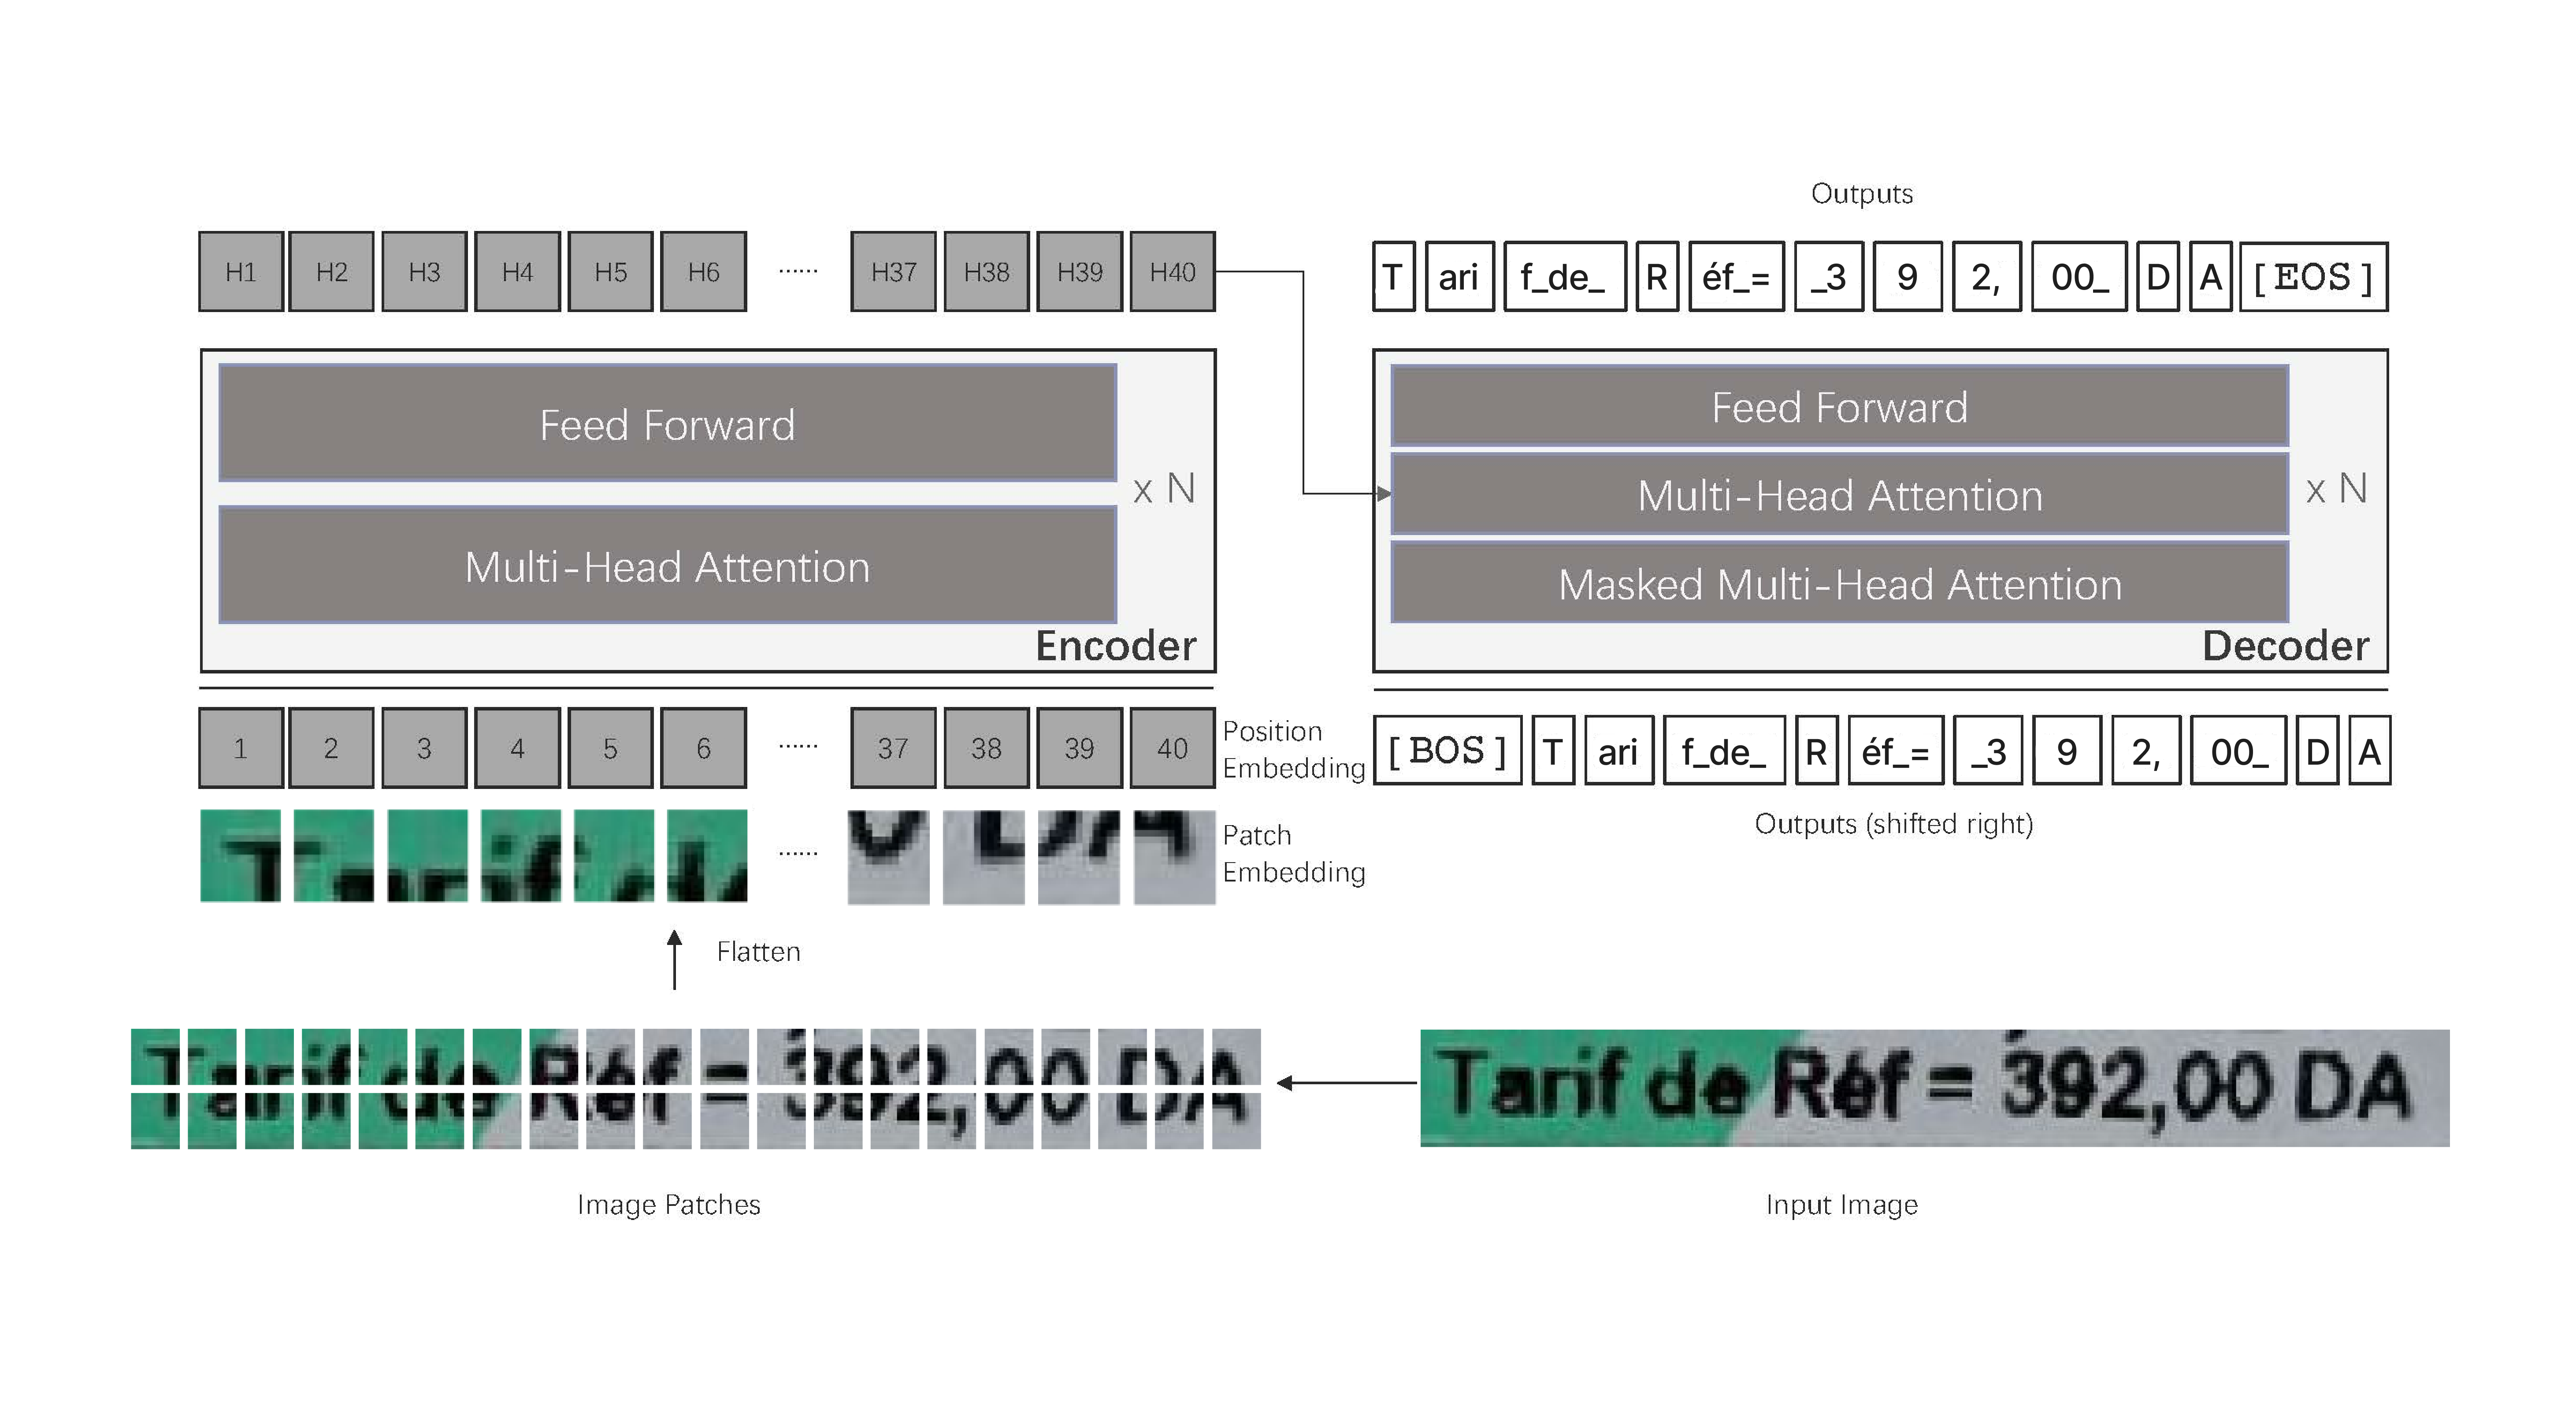
\includegraphics[width=1.10\textwidth]{Figures/Chapter 3/trocr_architecture.png}
    \caption{TrOCR Architecture}
    \label{fig:TrOCRArchitecture}
\end{figure}


\subsubsection*{1. Input Image and Patch Embedding}

The input image containing text (e.g., \textit{"Tarif de Réf = 392,00 DA"}) is first divided into a sequence of fixed-size image patches. Each patch is flattened and passed through a linear projection layer to obtain a \textit{patch embedding}. To preserve the spatial structure of the image, \textit{positional embeddings} are added to the patch embeddings.

\subsubsection*{2. Encoder (Vision Transformer)}

The encoder is a Vision Transformer (ViT), composed of multiple layers of:
\begin{itemize}
    \item \textbf{Multi-Head Self-Attention}, which allows the model to capture contextual relationships between different patches in the image.
    \item \textbf{Feed Forward layers}, which refine the representations of each patch.
\end{itemize}

The encoder transforms the sequence of embedded patches into a contextualized sequence of visual features \( H_1, H_2, \dots, H_{40} \).

\subsubsection*{3. Decoder (Text Transformer)}

The decoder is a Transformer decoder that generates the text sequence autoregressively. It consists of:
\begin{itemize}
    \item \textbf{Masked Multi-Head Attention}, which ensures that the decoder attends only to previously generated tokens.
    \item \textbf{Cross Attention}, which allows the decoder to focus on relevant parts of the encoder output.
    \item \textbf{Feed Forward layers}, which produce the final output representations.
\end{itemize}

The decoder starts with a special token \texttt{[BOS]} (beginning of sequence) and continues generating tokens until it predicts the \texttt{[EOS]} (end of sequence) token.

\subsubsection*{4. Output Sequence}

The final output is a sequence of text tokens that represent the transcribed content from the image. In the example shown, the model successfully generates:
\[
\texttt{Tarif\_de\_Réf\_=\_392,00\_DA}
\]

Each token is generated one at a time, using both the previously generated tokens and the visual context provided by the encoder.

\subsubsection{Dataset Configuration}
TrOCR fine-tuning dataset requires only the lines of text from Figure \ref{fig:segmentationoflabels} and a Txt File that contains the name of the images and the Corresponding ground truth next to it.

\begin{figure}[H]
    \centering
    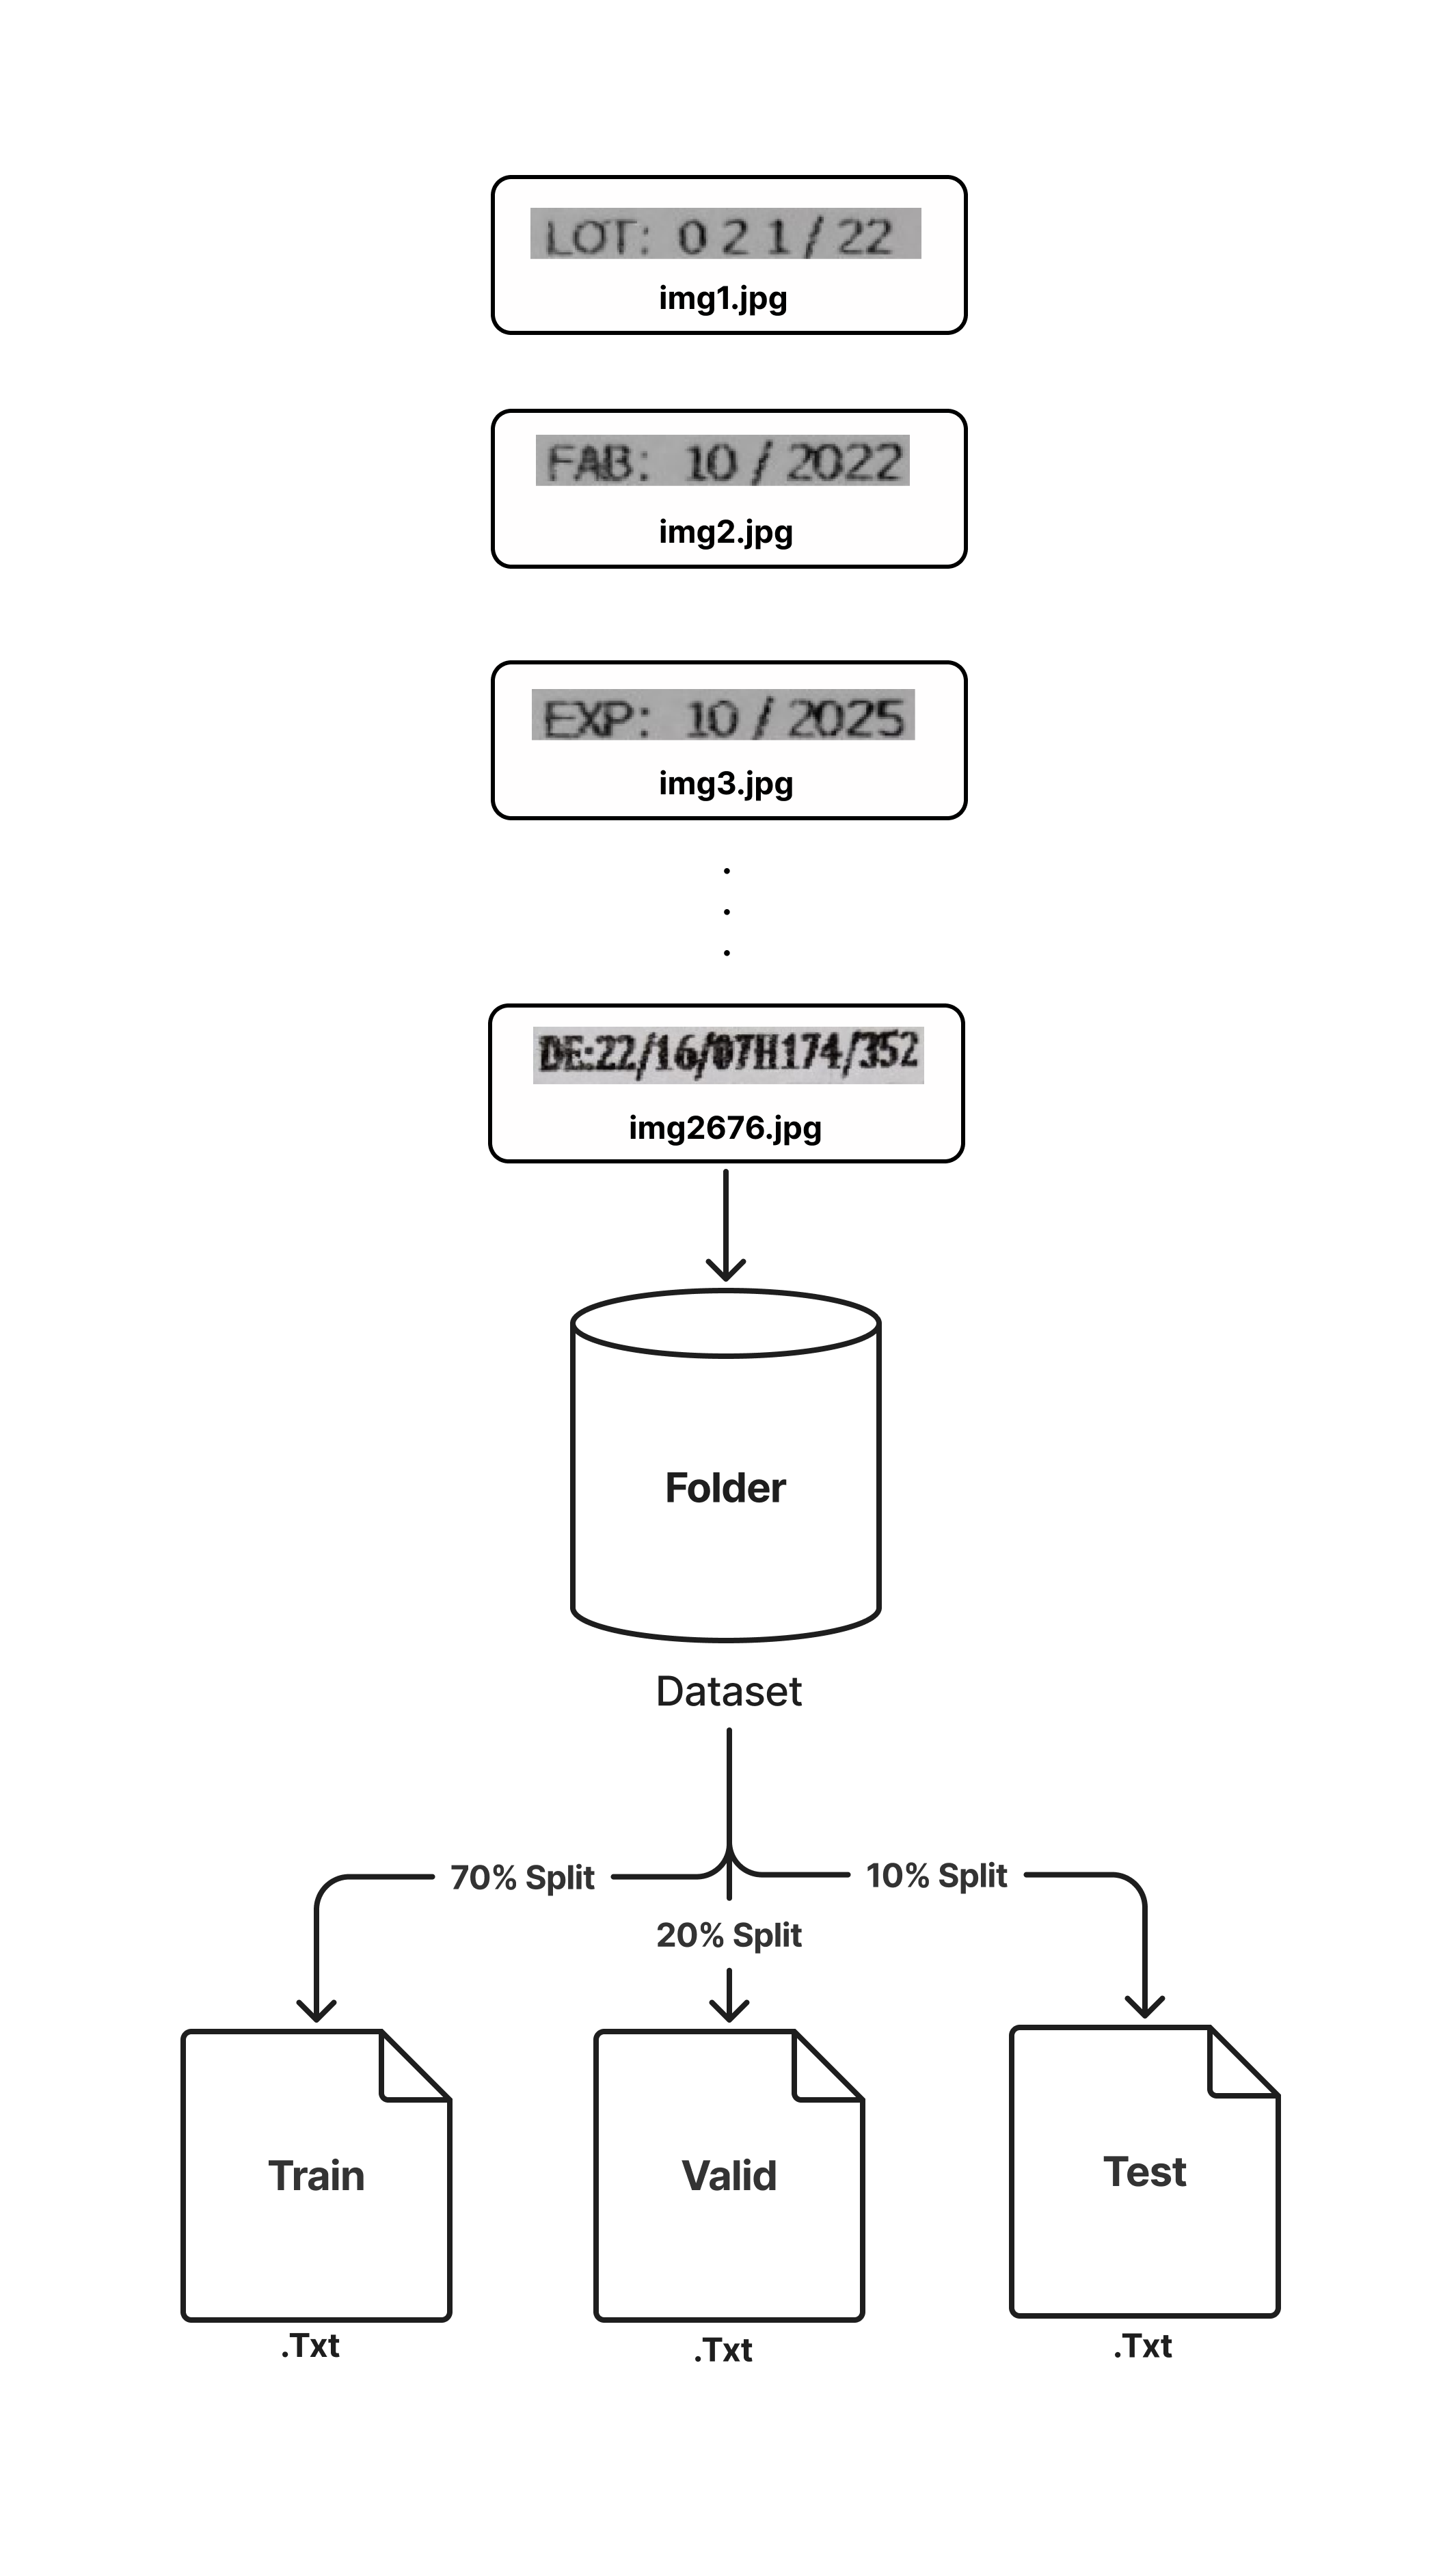
\includegraphics[width=0.50\textwidth]{Figures/Chapter 3/trocr_dataset_configuration.png}
    \caption{TrOCR Dataset Configuration}
    \label{fig:TrOCRdatasetconfiguration}
\end{figure}

\subsubsection{Standard TrOCR}

TrOCR leverages a transformer-based architecture for end-to-end text recognition,  but it occasionally struggles with domain-specific terms like the Algerian Medical Labels and low-quality scans, leading to partial misreads or omissions.

\begin{figure}[H]
    \centering
    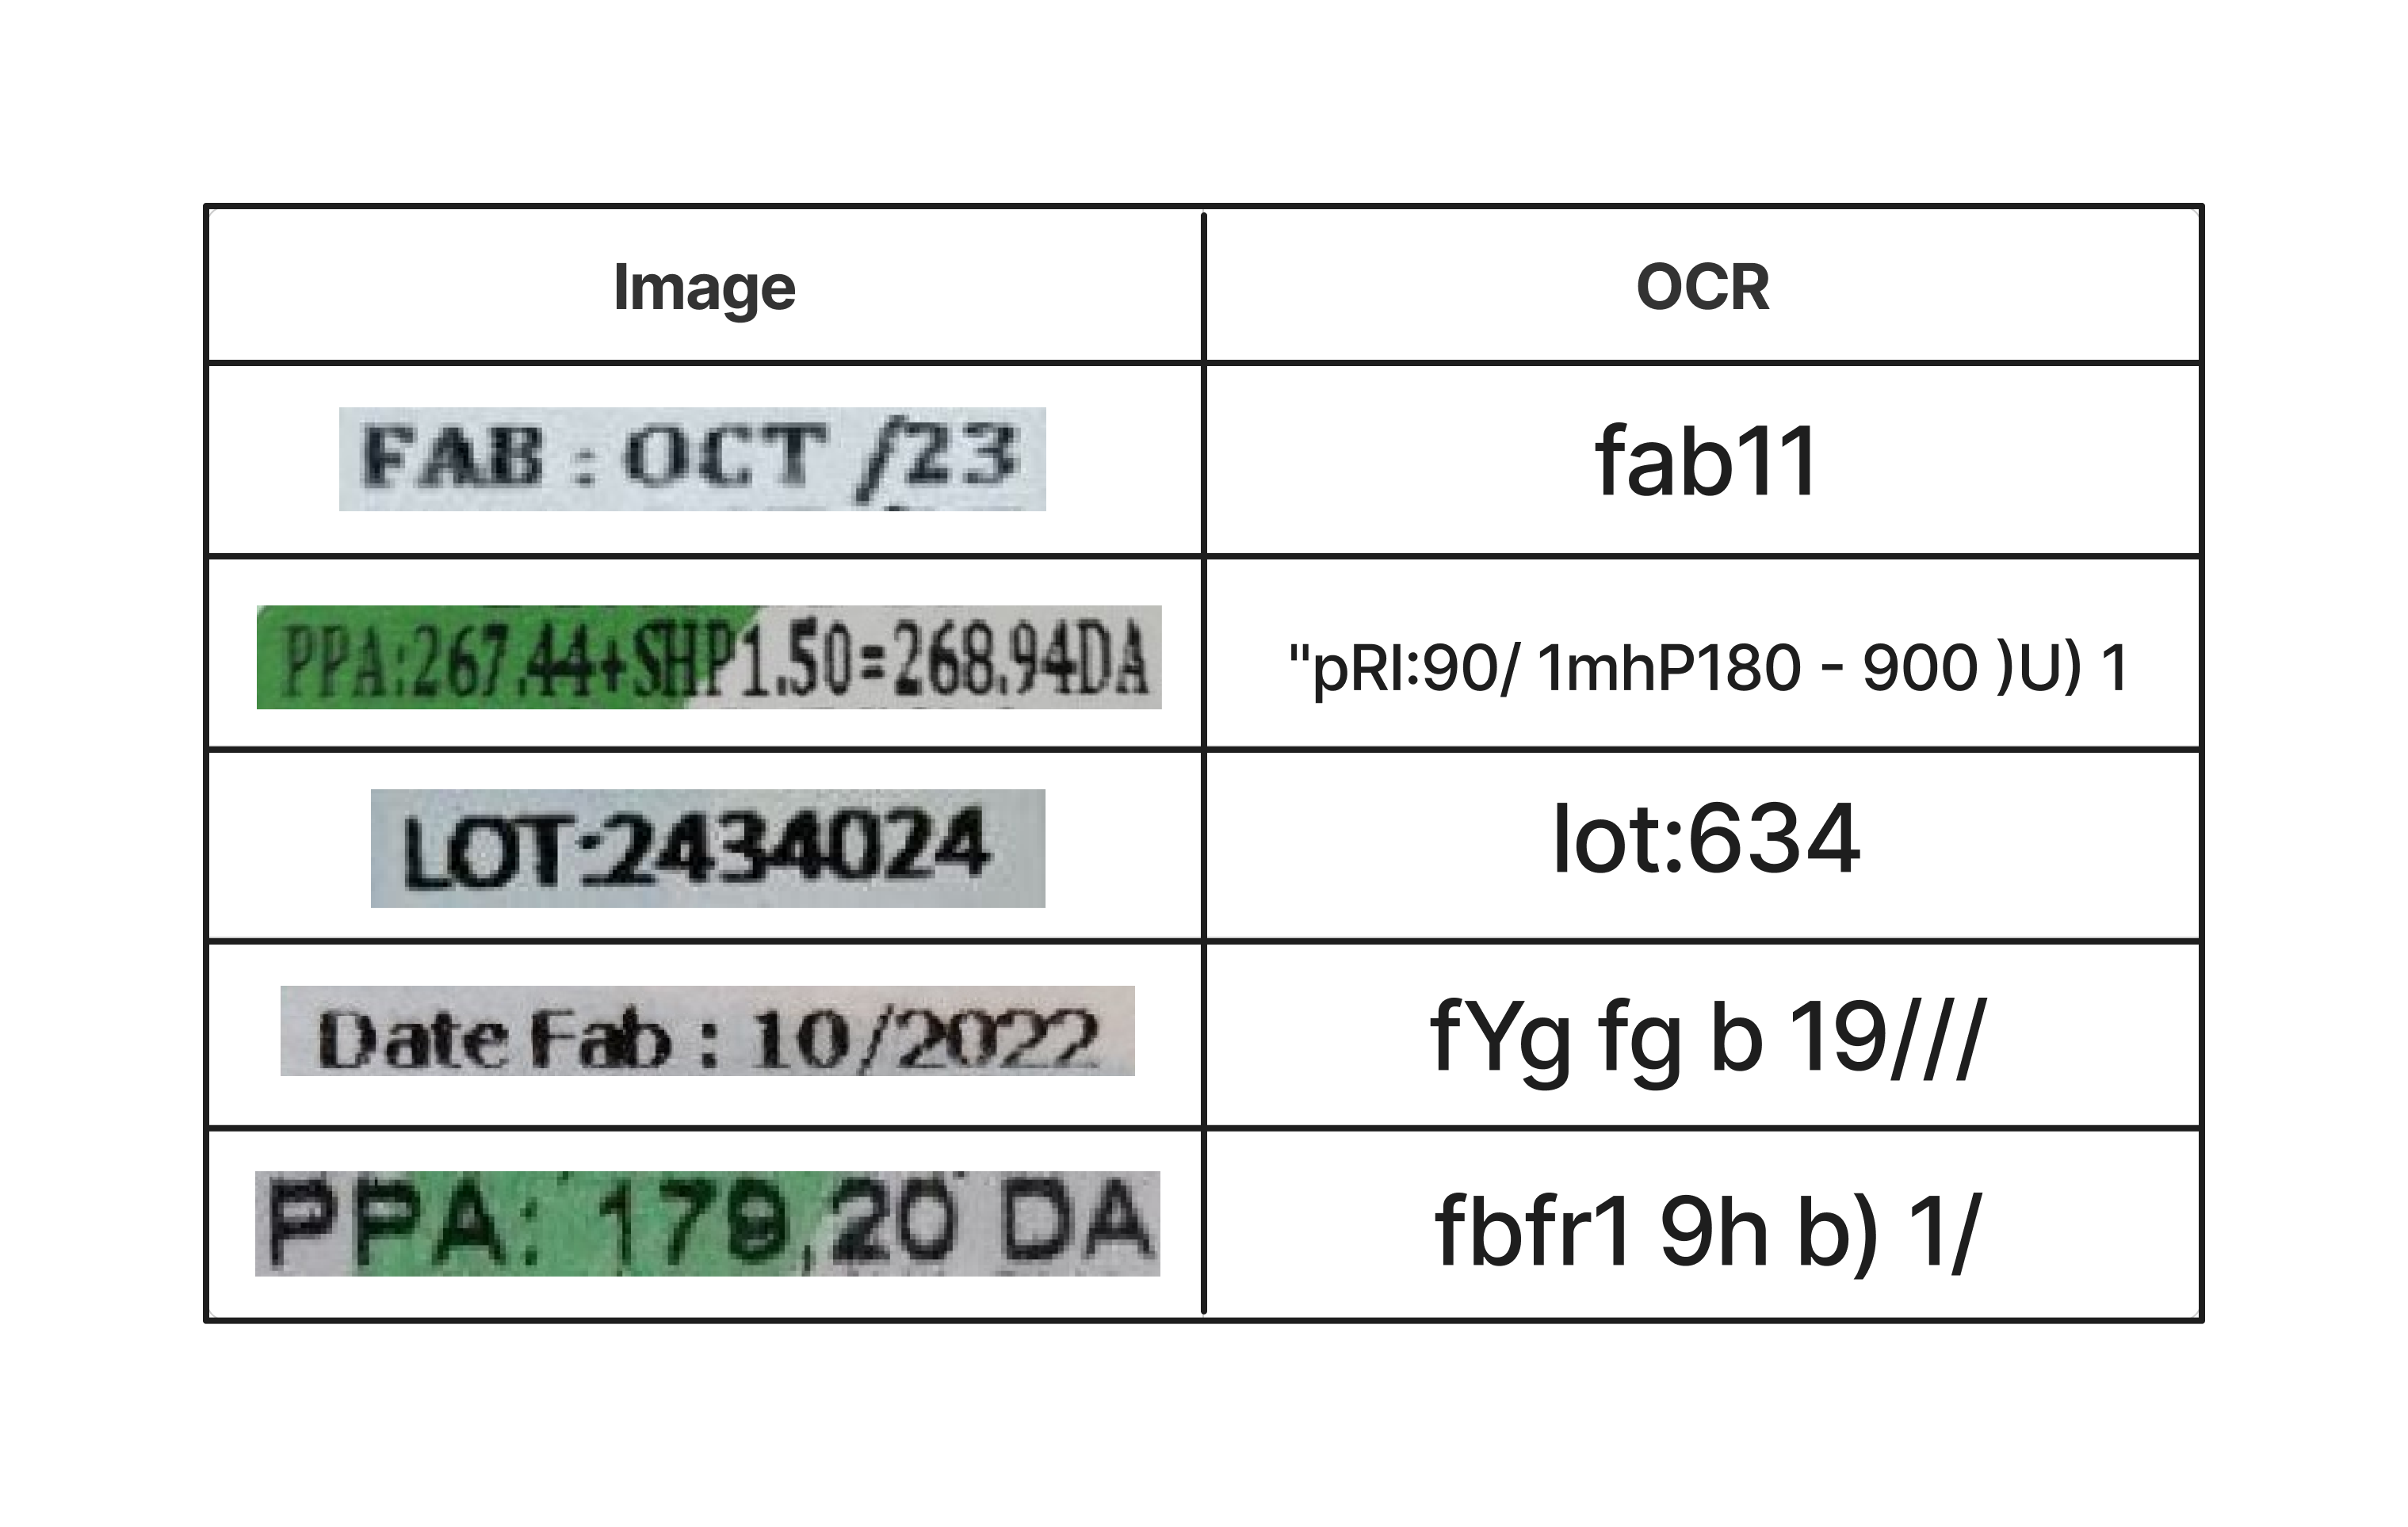
\includegraphics[width=0.75\textwidth]{Figures/Chapter 3/standard_trocr_results.png}
    \caption{TrOCR results on a test sample}
    \label{fig:TrOCRresultstestsample}
\end{figure}

The results shown in Figure~\ref{fig:TrOCRresultstestsample} are relatively more accurate compared to Figures~\ref{fig:standardeasyocrresults} and~\ref{fig:tesseractocrtestsample},. While not perfect, the standard TrOCR model handles the structure and language of Algerian medical labels better than Tesseract and EasyOCR. This improvement will be further supported and analyzed in the comparison study later in this chapter.


\subsubsection{Fine-Tuned TrOCR}

\subsubsection*{Fine-Tuning Results}

The fine-tuning process was conducted over 20 epochs using our custom dataset of Algerian medical labels. The evolution of the model's performance is illustrated through two key metrics: loss (training and validation) and the Character Error Rate (CER).

\begin{figure}[H]
    \centering
    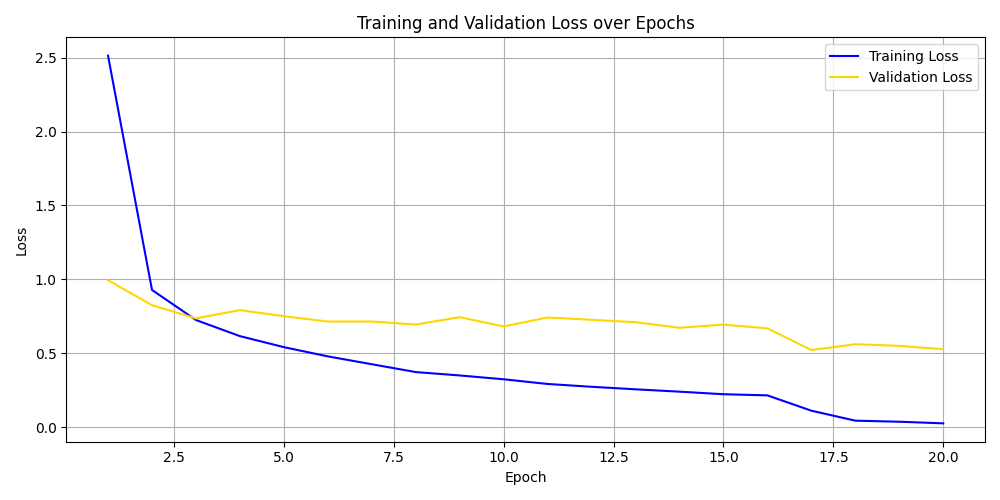
\includegraphics[width=0.85\textwidth]{Figures/Chapter 3/trocr_training_validation_loss.png}
    \caption{TrOCR Training and Validation Loss over Epochs}
    \label{fig:trocrtraining_validation_loss}
\end{figure}

Figure~\ref{fig:trocrtraining_validation_loss} shows that the training loss decreased steadily, indicating effective learning throughout the epochs. The validation loss initially fluctuated but gradually followed a downward trend, demonstrating that the model generalizes better over time. A significant drop in both training and validation loss occurred after epoch 15, highlighting a potential convergence point where the model becomes more stable.

\begin{figure}[H]
    \centering
    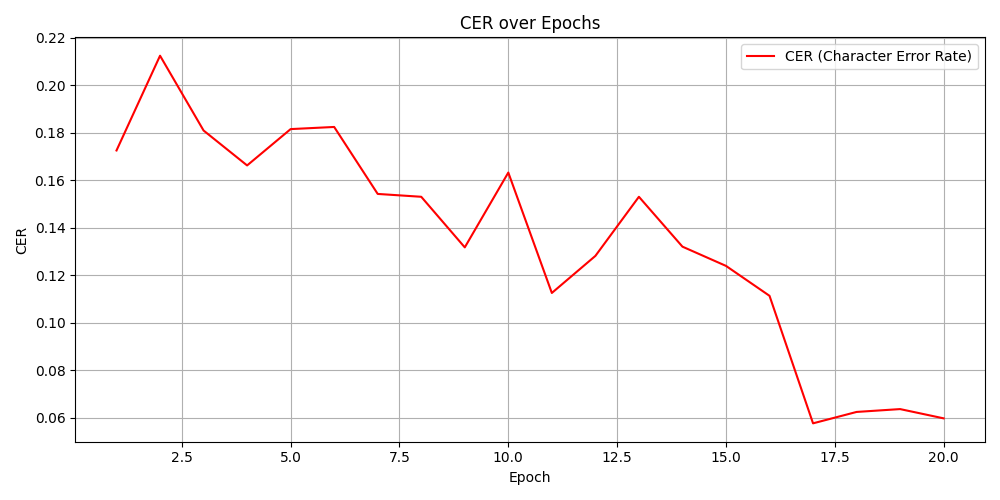
\includegraphics[width=0.85\textwidth]{Figures/Chapter 3/trocr_cer_over_epochs.png}
    \caption{TrOCR Character Error Rate (CER) over Epochs}
    \label{fig:trocrcer_over_epochs}
\end{figure}

Figure~\ref{fig:trocrcer_over_epochs} presents the CER across epochs. The model shows progressive improvements, with the CER dropping significantly after epoch 10 and reaching its lowest point at epoch 16. 

\subsubsection{Standard vs. Fine-Tuned TrOCR Comparison}
After the fine-tuning has completed, we performed a comparison study between the Standard and Our Fine-Tuned TrOCR model. The study was done using our Testing Set (10\% Split) and we summarized the results on 2 Tables.

\vspace{0.5cm}
\begin{table}[H]
\caption{Pretrained vs Fine-Tuned CER comparison on TrOCR Models}
\centering
\begin{tabular}{lc}
\hline
\textbf{Model Version} & \textbf{CER}  \\
\hline
Standard TrOCR & 0.7915 \\
Fine-Tuned TrOCR & 0.2451 \\
\hline
\end{tabular}

\label{tab:trocr-cer-comparison}
\end{table}


\vspace{0.5cm}
\begin{table}[H]
\caption{Sample Predictions: Standard vs. Fine-Tuned TrOCR}
\resizebox{\textwidth}{!}{
\centering
\begin{tabular}{llll}
\hline
\textbf{Image} & \textbf{Ground Truth} & \textbf{Fine-Tuned Prediction} & \textbf{Standard Prediction} \\
\hline
img873.jpg & BINOZYT 250mg & BINOzYT 250mg & biin g \\
img1132.jpg & PPA:267,44+SHP1,50=268,94DA & PPA:267 A4+SHP1,5O:268,94D4 & "pRI:90/ 1mhP180 - 900 )U) 1 \\
img1780.jpg & PPA+SHP=447.5+2.50 & PPA+SHP=447,5+2,50 & pbr gbD4 6N 80 \\
img2217.jpg & N°D.E: & NTD-e: & vi e3 \\
img1343.jpg & COXIBREX & COXiBrEX & v i nn b e f b \\
\hline
\end{tabular}}

\label{tab:trocr-sample-predictions}
\end{table}

As shown in Table \ref{tab:trocr-cer-comparison}, the fine-tuned TrOCR model achieved a significant improvement over the standard pretrained version, reducing the Character Error Rate (CER) from 0.7915 to 0.2451 — a relative improvement of 69.04\%. 

Table \ref{tab:trocr-sample-predictions} further illustrates this improvement with qualitative examples. While the standard model often failed to recognize meaningful tokens, the fine-tuned version produced much more accurate and readable outputs.

\section{Overview: Comparison Study of the Proposed Models}

To evaluate the effectiveness of fine-tuning, we conducted a comparative study between the standard (pretrained) and fine-tuned versions of each OCR model: Tesseract, EasyOCR, and TrOCR. All models were tested using the same testing set, and performance was measured using the Character Error Rate (CER), along with training time and final model size. The comparison results are presented in tables \ref{tab:cer-comparison-all} and \ref{tab:metrics-comparison}.

\vspace{0.5cm}
\begin{table}[H]
\caption{OCR models Comparison study }
\centering
\resizebox{\textwidth}{!}{
\begin{tabular}{lccccc}
\hline
\textbf{Model} & \textbf{Standard CER} & \textbf{Fine-Tuned CER} & \textbf{Improvement (\%)} & \textbf{Training Time} & \textbf{Model Size} \\
\hline
Tesseract & 0.8824 & 0.3142 & 64.40\% & \textbf{5 minutes} & \textbf{9,215 KB} \\
EasyOCR & 0.8627 & 0.2983 & 65.40\% & 10 minutes & 33,096 KB \\
TrOCR & \textbf{0.7915} & \textbf{0.2451} & \textbf{69.04\%} & 32 minutes & 240,655 KB \\
\hline
\end{tabular}}

\label{tab:cer-comparison-all}
\end{table}

\vspace{0.5cm}
\begin{table}[H]
\caption{Performance Metrics comparison for Fine-Tuned OCR Models}
\centering
\begin{tabular}{lccc}
\hline
\textbf{Metric} & \textbf{Tesseract} & \textbf{EasyOCR} & \textbf{TrOCR} \\
\hline
Character Error Rate (CER) & 0.3142 & 0.2983 & 0.2451 \\
Training Accuracy & 67\% & - & - \\
Validation Accuracy & 61\% & - & - \\
Training Loss & - & 34\% & 2\% \\
Validation Loss & - & 55\% & 52\% \\
\hline
\end{tabular}

\label{tab:metrics-comparison}
\end{table}

In Table~\ref{tab:cer-comparison-all}, all three models benefited significantly from fine-tuning on our domain-specific dataset of Algerian medical labels. TrOCR achieved the highest improvement, with a reduction of 69.04\% in CER, which is largely attributed to its transformer-based architecture and strong language modeling capabilities. EasyOCR also performed very well, maintaining a good trade-off between accuracy and training efficiency. However, both models are time-consuming when it comes to training and have a large model size.

Although Tesseract remains the least accurate, it still saw a substantial reduction in CER after fine-tuning. Its main advantage lies in its small size and extremely fast training time, making it a lightweight option for resource-constrained environments.

These findings emphasize the value of model adaptation for OCR in specialized domains. While deep learning models like TrOCR and EasyOCR yield superior recognition performance, practical considerations such as training time and model size may influence the choice of OCR engine based on deployment needs.

Further insights are provided in Table~\ref{tab:metrics-comparison}, which presents the metrics used to evaluate the performance of these models, obtained during the fine-tuning process. TrOCR achieved the lowest training and validation loss, confirming its efficiency in learning from the data with minimal overfitting. Although specific accuracy metrics were not logged for EasyOCR and TrOCR, the low CER values indirectly reflect their strong performance. Tesseract showed moderate training and validation accuracy (67\% and 61\% respectively), but still lagged behind in overall error rate. These results reinforce the idea that transformer-based architectures like TrOCR offer the most accurate recognition, while conventional engines like Tesseract may serve better in low-resource scenarios.


\section{Conclusion}

This chapter presented a comprehensive study on fine-tuning three OCR models—Tesseract, EasyOCR, and TrOCR—on a domain-specific dataset of Algerian medical labels. The experimental results demonstrate that adapting pretrained OCR models to specialized datasets significantly improves recognition accuracy, as evidenced by substantial reductions in Character Error Rate (CER) across all models.

TrOCR, leveraging a powerful transformer-based architecture, achieved the best overall performance with a 69.04\% improvement in CER, highlighting its strong capability in modeling complex visual and sequential information. EasyOCR also showed impressive gains, balancing accuracy and training efficiency, while Tesseract offered a lightweight and fast training alternative with moderate accuracy enhancements.

The comparison study emphasizes that fine-tuning is essential for OCR applications in specialized domains, where general pretrained models fall short due to unique visual patterns, fonts, and terminologies. Ultimately, the choice of OCR engine should consider the specific use case, balancing accuracy, model size, and computational resources.
\clearpage